\documentclass[a4paper,12pt]{article} \usepackage{a4wide}
\usepackage[cp1251]{inputenc}
\usepackage[english,russian,ukrainian]{babel}
\usepackage{amsfonts,amssymb,amsmath,amsthm,amscd,latexsym}
\usepackage{graphicx} \usepackage[matrix,arrow,curve]{xy}
% \pagestyle{headings}
\usepackage{fancyhdr} \fancyfoot{} \rhead{\thepage} \cfoot{} \lhead{}
\renewcommand{\headrulewidth }{ 0pt} \pagestyle{fancy} \sloppy
\parindent = 1 cm \topmargin - 16mm \textwidth 160mm \textheight 250mm
\oddsidemargin 10mm \evensidemargin 7mm
\newcommand*{\hm}[1]{#1\nobreak\discretionary{}%
  {\hbox{$\mathsurround=0pt #1$}}{}} \newcommand{\bb}[1]{{\bf #1}}
\renewcommand{\theequation}{\thesection.\arabic{equation}}
\numberwithin{equation}{subsection}
\newtheorem{theorem}{Теорема}[subsection]
\newtheorem{lemma}{Лема}[subsection]
\newtheorem{corollary}{Наслідок}[subsection]
\newtheorem{remark}{Зауваження}[subsection]
\newtheorem{definition}{Означення}[subsection]
\newtheorem{example}{Приклад}[subsection]
\newtheorem{hyp}{Гіпотеза}[subsection]
\renewcommand{\baselinestretch}{1.5}

\graphicspath{{../Pictures/}}

\begin{document}

\begin{titlepage}
  \vspace*{0.2cm}
  \begin{center}
    Національний Університет "Києво-Могилянська Академія"
  \end{center}
  \vspace{0.6cm}
  \begin{flushright}
    На правах рукопису
  \end{flushright}
  \vspace{1cm}
  \begin{center}
    Морозов Денис Іванович
  \end{center}
%
  \begin{flushright}
    УДК 512.54
  \end{flushright}
%
%
  \begin{center}
    \textbf{Скінченностанова спряженість ізометрій простору 2-адичних
      чисел}

    \vspace{0.5cm}

    01.01.06 -- алгебра та теорія чисел
  \end{center}
%
%
  \vspace{1 cm}
  \begin{center}
    Дисертація на здобуття наукового ступеня \\ доктора  фізико--математичних наук \\
  \end{center}

  \vspace{8 cm}


\begin{center}
  Київ
\end{center}
\end{titlepage}

\setcounter{page}{2}
\tableofcontents
\newpage
\section*{Перелік умовних позначень}
\addcontentsline{toc}{section}{Перелік умовних позначень} \bigskip
\begin{tabular}{ p{2.4in} p{3.5in} }
  \
  $\mathbb{N}^+$ & - напівгрупа натуральних чисел  по додаванню ; \\
  $\bar{\mathbb{N}}^+ = \mathbb{N}^+ \cup \{ 0 \}$ & - напівгрупа натуральних чисел з нулем; \\
  $Z_p$ & -кільце цілих p-адичних чисел;\\
  $Z_T$ & -кільце розширених по дереву $T$ цілих 2-адичних чисел ;\\
  $C_n^{(r)} $& -декартів добуток $r$ копій циклічної групи $C_n$;  \\




  $G \ltimes H $ & - напівпрямий добуток груп , де $H-$ нормальний дільник ; \\
  $\left(G,X \right) \imath  H $ & -вінцевий добуток групи перетворень $\left(G,X \right)\ $(активний співмножник) та
  абстрактної групи $H$; \\


  $<M,g,\ldots > $ &- підгрупа породжена множиною $M$ та елементами $g,\ldots $; \\
  $K^+, K^* $ & - адитивна та мультиплікативна групи поля ; \\

\end{tabular}

\begin{tabular}{ p{2in} p{3.5in} }








  $\circ$& -суперпозиція автоморфізмів, функцій. \\
  $T_n $&- кореневе однорідне дерево валентності $n$ ;\\
  $AutT_n $&- група автоморфізмів кореневого однорідного дерева валентності $n$ ;\\
  $FAutT_n $&- підгрупа скінченностанових автоморфізмів групи  $AutT_n $;\\
  $STAutT_n $&- Множина шарово-транзитивних автоморфізмів групи  $AutT_n $;\\
  $\zeta(a) $&- кількість різних станів автоморфізму a ;\\

  $C_G(a)$&- централізатор елемента $a$ в групі $G$;\\
\end{tabular}
\newpage
\section*{Вступ}
\addcontentsline{toc}{section}{Вступ}


Наприкінці  двадцятого сторіччя на стику алгебри, дискретної математики та топології виник новий напрямок
досліджень, який можна охарактеризувати як динаміку алгебраїчних структур. Він акумулював в собі дослідження
самоподібності таких структур, їх функцій росту, автоматні перетворення, дії на графах, зокрема на деревах,
наявність інваріантних мір, ймовірносні розподіли та випадкові блукання на таких структурах. Серед засновників
цього напрямку такі відомі математики як М. Громов, Ж.-П. Серр, Ж. Тітс, Р. Григорчук, С. Сідки, Н. Гупта, В.
Сущанський.

Вивчення групових дій на нескінченних деревах займає тут чільне
місце
%  і  конференція "Groups generated by automata", що відбулася
% цього року в Асконі (Швейцарія) підтвердила це
. Базовим  є
приклад бінарного однокореневого нескінченного дерева $T_2$, група
автоморфізмів якого $Aut T_2$ збігається з проективною границею
ітерованих вінцевих добутків циклічних груп другого порядку. Ця
група є топологічною, як про-2-група. Нескінченні шляхи, що
виходять з кореневої вершини можна ототожнити з нескінченними
двійковими послідовностями, як елементами метричного простору Бера
над двоелементним алфавітом. При цьому вказана група буде також
групою ізометрій цього простору. Кожній вершині цього дерева
відповідає скінченна послідовність нулів та одиниць $w$- шлях від
кореневої вершини до даної. Автоморфізм дерева $\sigma$ переводить
всі кінці з початком $w$ переведе в кінці зі спільним початком
$w',$ тобто для довільної нескінченної двійкової послідовності
кінець $w x,$ буде перетворений автоморфізмом в кінець $w' y, $
причому відображення $x \to y=y (x)$ є також автоморфізмом
нескінченного бінарного дерева. Всі автоморфізми дерева отримані з
$\sigma$ у вказаний спосіб називаються {\bf станами} автоморфізму
$\sigma$. Особливо цікавими є скінченностанові автоморфізми, які
утворюють групу, про будову якої відомо дуже мало.\cite{Gr1}

Дисертація присвячена дослідженню проблеми спряженості елементів в цій групі. Слід зауважити, що в усій групі
автоморфізмів дерева ця проблема легко розв'язується за допомогою  циклового дерева  - аналога циклового типу
підстановки. Як відмічають фахівці в загальній постановці проблема спряженості в групі скінченностанових
автоморфізмів є дуже важкою.

%  Проведене дослідження обмежується таким важливим і природним класом автоморфізмів
% як лінійні ізометрії.

 Якщо ототожнити кінці дерева з цілими 2-адичними числами, то будь-який автоморфізм дерева
визначає ізометрію кільця  цілих 2-адичних чисел $Z_2$ з 2-адичною метрикою. При цьому структура кільця
дозволяє розглядати лінійні перетворення $ x \to a x +b, x,b \in Z_2, a \in Z_2^*. $ Такі перетворення ми і
називаємо лінійними ізометріями.

Встановлено, що вони є скінченностановими тоді і лише тоді, коли $a,b$ є раціональними числами (лема 4.2.4).

Для розв'язання проблеми скінченностанової спряженості даних автоморфізмів $\alpha,\beta$ слід з'ясувати
існування скінченностанових розв'язків  $\theta$ рівняння $\theta^{-1} \alpha \theta = \beta.$ Оскільки
розв'язки відрізняються на елементи з централізатора $\alpha$, то дослідження розпочинається з дослідження
будови централізаторів автоморфізмів.  Ці централізатори очевидно є замкненими підгрупами в топології
проективної границі на групі $Aut T_2$. Особливо прозорою вона стає для елементів максимального пропорядку, для
яких вказана вище підстановка $w \to w'$ є повним циклом на кінцях всіх "зрізаних" дерев і дерево циклового
типу є ланцюгом. Для таких елементів має місце

 \textbf{Теорема 3.3.3}
\emph{Нехай $ w$- довільний елемент максимального
  про-порядку і $D(w)= \{ w^k\mid k\in \mathbb{Z} \} -$ циклічна група породжена цим елементом,
   тоді $ C_{\overline{W}_\infty}(w)=\overline{D(w)}$,
   де риска означає замикання у топології про-2-групи.}


Для інших елементів у яких дерево циклового типу не є ланцюгом, опис централізатору є складнішим. Природним
чином вводиться структура кільця   на деревах циклового типу розмічених нулями та одиницями. Такі дерева ми
будемо називати розширеними 2-адичними числами. Тоді має місце

\textbf{Теорема 3.4.4}
\emph{$C_{AutT_2}(a)\cong H_a\leftthreetimes K_a$},

  де $H_a$ ізоморфна адитивній групі кільця розширених 2-адичних чисел по дереву циклового типу елемента a ,
  а $K_a$ ізоморфно групі автоморфізмів дерева циклового типу елемента a.





Використовуючи наведений опис централізаторів скінченностанових автоморфізмів максимального про-порядку
  $T_2$, які задаються лінійними ізометріями на
$Z_2$ отримаємо наступні результати

 \textbf{Лема 4.2.4}

  \emph{ Всі функції $f(x)=ax+p,(a,p\in
(Z_2\cap{\mathbb{Q}})^*  )$ спряжені з функцією $f(x)=ax+1$  в
$FAutT_2$}




 \textbf{Теорема 4.2.5}
 \emph{Функції $f_1(x)=(4k_1+1)x+1$ та $f_2(x)=(4k_2+1)x+1 \ (k_1,k_2 \in
Z_2\cap\ {\mathbb{Q}})$ спряжені в $FAutT_2$ тоді, і тільки тоді,
коли $ 4k_1+1=4k_2+1.$ }

тобто скінченностанові автоморфізми максимального про-порядку, що
задаються лінійними
 функціями $ax+c,\ bx+d\ (a,b,c,d\in Z_2)$ спряжені в $FAutT_2$ тоді і тільки тоді, коли
  $a=b$.

\begin{example}
Функції $f(x)=x+1$ та $f(x)=5x+1$ спряжені в групі автоморфізмів
бінарного дерева, оскільки мають ізоморфні дерева циклового типу,
але не спряжені в скінченностановій підгруппі цієї групи.

 Дійсно, єдиний розв"язок $$\theta_0(x)=\frac{5^x-1}{4}$$ рівняння $$\theta^{-1}\circ(x+1)\circ \theta=5x+1)$$
 що залишає 0 на місці, переводить квазіперіодичне(раціональне) 2-адичне
 число $\frac{1}{3}$
 в неперіодичне(іраціональне) 2-адичне число $\frac{\sqrt[3]{5}-1}{4}$, а отже є нескінченно
 становим. Звідси випливає, що скінченностанових розв"язків немає
 взагалі. Припустимо, що є скінченностановий розв"язок $\theta_p$, що переводить квазіперіодичне(раціональне) 2-адичне
 число p в
 0. Функцію $\theta_p$ представимо, як добуток елементу
 централізатору $C_{FautT_2}(f(x)=x+1)$ на $\theta_0$:$$\theta_p=(x-p)\circ \theta_0
 .$$ Оскільки p - раціональне, то $f(x)=x-p$- скінченностановий автоморфізм,
 отже $\theta_p$- нескінченностановий.

\end{example}










% Дослідження проводились в рамках науково дослідної теми
% "Перетворення Кремони та локально-нільпотентні диференціювання
% алгебр поліномів: теорія та застосування в надлишковому кодуванні
% інформації та криптографії", що виконує кафедра математики НаУКМА
% на замовлення Державного Фонду Фундаментальних досліджень(
% реєстраційний номер 0107U010499).


Результати дисертаційної роботи мають теоретичний характер і можуть бути використані для подальших досліджень з
проблеми скінченностанової спряженості.

 Вони опубліковані в наступних статтях:


% Вони опубліковані в п'яти статтях, три з яких в журналах з переліку ВАК. Теореми  3.3.2, 3.3.3 та 3.3.4 були отримані спільно з
% науковим керівником, який для їх доведень запропонував техніку проективних замикань. Решта результатів отримано
% самостійно.
{ Скінченно-станова спряженість сферично-транзитивних
  автоморфізмів кореневого бінарного дерева.
Науковий часопис НПУ імені М.П.Драгоманова. Cерія 1.
Фізико-математичні науки // Київ: НПУ імені М.П. Драгоманова. -
2013, № 12, C.~5-12}


{ Спряженість транзитивно-стабільних
  автоморфізмів в $FAutT_2$.
Науковi записки
  НаУКМА. Фізико-математичні науки.  - 2012.  Том 126. C.~7-9. }


{ Централізатори шарово-транзитивних елементів в групі скінченно-станових автоморфізмів бінарного кореневого дерева.
Вісник Київського університету//Серія: фізико-математичні науки.-2012}

{ Морозов Д.I.  Ізометричність поліномів над кільцем цілих
  2-адичних чисел //Науковi записки НаУКМА. Фiзико-математичнi
  науки. - 2011.  Том 113. C.~13-15. }


{ Морозов  Д.I.  Спряженiсть  автоморфiзмiв,  що
задаються лiнiйними функцiями в групi скiнченностанових
автоморфiзмiв кореневого сферично-однорiдного дерева   //Вiсник
Київського   ун-ту. Серiя: фiзико-математичнi науки. - 2008.-
вип.№1 - C.~40-43.}


{ Морозов Д.I.  Скiнченностанова спряженiсть лiнiйних
  функцiй на кiльцi цiлих 2-адичних чисел /Боднарчук Ю.В., Морозов
  Д.I.// Доповiдi НАН України .  Фiзико-математичнi науки. - 2008. №9
  -C.~7-11. }

\bigskip

 Отримані результати доповідались:
%\begin{description}

% 5-та Міжнародна Алгебраїчна Конференція, м.Одеса, Україна

% 6-та Міжнародна Алгебраїчна Конференція, м.Кам'янець-Подільський, Україна

%  Міжнародна Алгебраїчна Конференція "Groups generated by automata", Ascona, Швейцарія

 Семінар  кафедри алгебри КНУ Шевченка.

 Семінар з фрактального аналізу Інституту математики НАН України.

IІ Всеукраїнський науковий семінар 
"Комбінаторна оптимізація та нечіткі множини", м.Полтава(тези,  Обчислення функції росту диференційовних ізометрій бінарного кореневого дерева. )

9th Int. Algebraic Conf. in Ukraine: Abstr. Lviv, July 8-13, 2013.( Abstracts, P. 132, Recursive criterion of conjugation of finite-state binary tree’s
automorphisms. ) 


International Conference on Algebra dedicated to 100th anniversary of S.M.Chernikov,
Dragomanov National Pedagogical University, Kyiv, Ukraine, August 20-26, 2012.( Abstr.  P. 96,  Conjugacy of piecewise-linear spherical-transitive automorphisms.)

 PDMU-2012,
XX International Conference PROBLEMS OF DECISION MAKING UNDER UNCERTAINTIES,
Brno, Czech Republic, September 17-21, 2012. (Abstr. Functional representation of automorphisms of rooted spherical homogeneous tree.)

 8th Int. Algebraic Conf. in Ukraine. Lugansk, July 5-12,
2011.( Abstr. P. 116 Differentiable finite-state izometries and izometric polynomials of the ring
of integer 2-adic numbers. )


2nd Inter-University Scientific Conference of Young Scientists in Mathematics and
Physics. Kiev, April 28-29, 2011.( Hausdorff s dimension of limit s set of compressive mappings semigroup.)

Ukrainian Mathematical Congress, 7th Int.
Algebraic Conf. in Ukraine: Abstr. Kiev, August 18-23, 2009. (Abstr. P. 97. Finite state conjugation of linear functions on the ring of n-adic integer
numbers.)

7th Int. Algebraic Conf. in Ukraine: Abstr. Kharkiv, August 13-17, 2009.
(Abstr. P. 110. Morozov Denis, Linear function which are conjugated in the group FAutT2 of finite state
automatous. )

%\end{description}



\newpage

\section{Попередні відомості}
\subsection{Ізометрії простору Бера як автомофізми дерев.}
Нагадаємо, що однокореневим деревом називаєься зв'язний граф без циклів з відміченою вершиною.
 Зауважимо, що автоморфізм кореневого дерева переводить відмічену вершину в себе.

Нехай X скінченний алфавіт. Простором Бера над алфавітом називається множина нескінчених послідовностей
$x_1x_2x_3..., x_i \in X$
з наступною метрикою:
  $$( x_1x_2x_3..., y_1y_2y_3...)=(\frac{1}{2})^k,$$  де k - довжина спільного початку
  $x_1x_2x_3...$ та $y_1y_2y_3...$ .
  \begin{example}
Розглянемо множину формальних сум вигляду:

\[
Z_p  = \{ \sum\limits_{k = 0}^\infty  {a_k  \cdot p^k } \left| {a_k  \in ,} \right.0 \le a_k  < p\}
\]

Відстань між елементами
\[
a = \sum\limits_{k = 0}^\infty  {a_k  \cdot p^k }
\]
та \[
b = \sum\limits_{k = 0}^\infty  {b_k  \cdot p^k }
\] цієї множини покладемо
\[
\rho (a,b) = \left( {\frac{1}{2}} \right)^k
\]
 де k визначається, як
\[
k = \mathop {\min }\limits_{t \in  \mathbb{N}\cup \{ 0\} } (a_t  \ne b_t )
\]
Таким чином визначена метрика перетворює $Z_p$ на простір Бера над p-літерним алфавітом.

\end{example}
  Співставимо простору Бера над p-літерним алфавітом регулярне однокореневе дерево $T_p$ за наступним правилом:
  кожній вершині відповідає скінчене слово в алфавіті X. Назвемо вершинами 1-го рівня вершини, що з'єднані з коренем
  одним ребром. Вершинами i-го рівня назвемо вершини, що з'єднані одним ребром з вершинами (i-1)-го рівня.

   Вершині i-го рівня відповідає слово довжини i.

   Легко зрозуміти , що група ізометрій такого простору ізоморфна групі автоморфізмів
    побудованого дерева.

    Охарактерізуємо її як абстрактну групу.


    Нехай $W_1=S_X$ - група підстановок на X, тоді
 можна індуктивно визначити групи $W_{n+1}=(W_n,X^n)\imath
 S_X$, як вінцевий добуток групи підстановок $W_n$, що діє на
  $X^n=X\times ...\times X$(активний співмножник)
  та групи підстановок на X. База вінцевого добутку
  складається з функцій $X^n\rightarrow X$ від $n$
  змінних і є ядром
  природного епіморфізму $\pi_n:W_{n+1}\rightarrow W_n$. Ці
  гомоморфізми визначають $ \overline{W}_\infty (X)$
  як проективну границю $ \overline{W}_\infty (X) = \underleftarrow {\lim} W_n, $
  а також гомоморфізми $\hat{\pi}_n: \overline{W} \to W_n.$
  При цьому група
  $\overline{W}_\infty$
  діє природним чином на  просторі Бера.
  Має місце наступна теорема:

  \begin{theorem}
  \cite{Sch1},\cite{Sch2}
   Група ізометрій простору Бера ізоморфна $ \overline{W}_\infty (X)$.
\end{theorem}
Елементи групи $\overline{W}_\infty $ можна  зображати
  нескінченними  послідовностями функцій:
\begin{equation} \label{sigmaseq}
   g=<\sigma_1,\sigma_2(x_1),\sigma_3(x_1,x_2), \ldots ,\sigma_k(x_1,x_2,...,x_{k-1}), \ldots >,
\end{equation}
   де $x_1,x_2,...,x_{k-1} -$ координати вершини $k-1-$ го рівня, а значенням функції $\sigma_k$ є одиниця,
   якщо відповідний автоморфізм дерева переставляє дві суміжні вершини $k-$ го рівня (див. вище п. в)) і є нуль
   якщо автоморфізм залишає ці вершини нерухомими.
   Аналогом циклового типу на групі підстановок є дерево циклового типу на $ \overline{W}_\infty (X)$.
   \begin{definition}
Елемент $a$ групи $\overline{W}_\infty $ задає розбиття множини вершин кожного рівня дерева $T_p$
 на множину орбіт дії цього елементу на $T_p$. Побудуємо по $a$ дерево циклового типу $D_a$ цього елементу. Вершинами цього дерева будуть
 класи еквівалентності по орбітах, причому дві вершини дерева $D_a$ з'єднані ребром, якщо існують суміжні вершини дерева $T_p$ з відповідних орбіт.
    \end{definition}
    Аналогом крітерія спряженості в групі підстановок є наступний крітерій в групі $ \overline{W}_\infty (X)$.
   \begin{theorem} \cite{Sch2}

 Елементи групи $ \overline{W}_\infty (X)$ є спряженими, якщо їх дерева циклового типу ізоморфні.
\end{theorem}
$ \overline{W}_\infty (X)$ є проскінченною групою і топологічною групою з топологією проективної границі.
\begin{theorem} \label{topgroup}
    $\overline{W}_\infty $- є повною топологічною групою.
\end{theorem}
\begin{proof}
     Покажемо, що  відображення
      \[ \overline{W}_\infty \times \overline{W}_\infty \rightarrow
      \overline{W}_\infty  \ \ \ (g_1,g_2)\rightarrow g_1\cdot g_2^{-1} \] є
    неперервним в цій топології.
Нехай $q_0 = g_1 \cdot g_2^{-1}$ і $B_{m}(q_0) = \{g | \rho(g,q_0) < 2^{- (m+1)} \}-$ відкрита куля з центром в $q_0.$
Легко бачити, що $\forall g_1,g_2 \in B_{m}(q_0)$ має місце $\hat{\pi}_m(g_1), \ \ \hat{\pi}_m(g_2).$ Розглянемо
довільні елементи куль $b_1  \in B_{m}(g_1), b_2 \in B_{m}(g_2).$ Для цих елементів буде мати місце $\hat{\pi}_m(b_1) =
\hat{\pi}_m(g_1), \ \ \hat{\pi}_m(b_2) = \hat{\pi}_m(g_2),$ звідки
\[ \hat{\pi}_m ( b_1 \cdot b_2^{-1}) = \hat{\pi}_m ( b_1) \cdot \hat{\pi}_m ( b_2)^{-1} =
\hat{\pi}_m ( g_1) \cdot \hat{\pi}_m ( g_2)^{-1} = \hat{\pi}_m ( g_1 \cdot  g_2^{-1}),\] отже, $b_1 \cdot b_2^{-1} \in
B_{m} (q_0).$ Це   доводить, що  $\overline{W}_\infty $ є топологічною групою. Для доведення повноти, слід зауважити,
що $\overline{W}_\infty $ є компактом у вищезгаданій топології, оскільки є замкненим у добутку дискретних просторів
$\hat{\pi}_m(\overline{W}_\infty ),m \in \mathbb{N}  $.
\end{proof}

   Група $ \overline{W}_\infty (X)$
   є самоподібною, в тому сенсі, шо мають місце факторізації $\overline{W}_\infty (X)=W_k\imath \overline{W}_\infty (X), k=1,2,3...$.
 \begin{definition} Елемент групи називається скінченностановим, якщо для всіх факторізацій елемента g
  $$g=w_k\cdot f_k(x_1...x_k)$$
  множина значень функцій, яку будемо називати множиною станів
  $$\{f_k(x_1...x_k)\mid x_1...x_k \in \overline{W}_\infty (X), k\in \mathbb{N}\}\subset \overline{W}_\infty (X)$$
  є скінченною.
    \end{definition}

 \begin{example}
 Очевидно, тотожній автоморфізм є одностановим.
\end{example}

\begin{example}
Зафіксуємо нескінченну послідовність $x_1^* x_2^* ... $  і автоморфізм $\sigma \in \overline{W}_\infty (X) $.
 Автоморфізм, для якого для всіх k $f_k(x_1^* x_2^* ...x_k^*)=\sigma$  та   дорівнює $id$ на інших векторах є двостановим.
\end{example}
 \begin{definition}
 Позначимо кількість \textbf{різних} станів автоморфізма a як $\zeta(a)$. Функцією зросту автоморфізму a називається функція $\varphi_a$, визначена наступним чином:
 $$\varphi_a(n)=\zeta(a^n)$$
 \end{definition}
  \begin{example}
  Для тотожнього автоморфізму, оскільки $id^n=id$ та $id=(id,id)$, то $\zeta(id^n)=\zeta(id)$. Тобто функція зросту для id має вигляд $\varphi_{id}(n)=1$.

   \end{example}
Означимо на множині функцій $\mathbb{N}\rightarrow \mathbb{N}$ бінарне відношення $\preccurlyeq$.
\begin{definition}\cite{Gr1}
Для функцій $\alpha:\mathbb{N}\rightarrow\mathbb{N}$ та $\beta:\mathbb{N}\rightarrow\mathbb{N}$ будемо казати,
що $$\alpha\preccurlyeq\beta$$ якщо знайдеться таке натуральне C, що для всіх натуральних n справджується
нерівність:
$$\alpha(n)\leqslant\beta(Cn).$$
 \end{definition}
 \begin{definition}

 Кажуть, що автоморфізми $a$ та $b$ мають однаковий зріст, якщо для функцій зросту $\varphi_a$ та $\varphi_b$ має місце:
 $$\varphi_a\preccurlyeq\varphi_b$$
$$\varphi_b\preccurlyeq\varphi_a$$




\end{definition}
\begin{lemma}

 Якщо існує скінчене ненульове C, таке, що для автоморфізмів a та b при всіх натуральних n має місце нерівність:


\[
\frac{1}{C} \le \frac{{\varphi _a (n)}}{{\varphi _b (n)}} \le C
\]
то автоморфізми $a$ та $b$ мають однаковий зріст.
\end{lemma}
З означення суперпозиції автоморфізмів випливає:

 \begin{lemma}
   Для функції $\zeta$ має місце нерівність: $$\zeta(a\circ b)\leqslant \zeta(a)*\zeta(b)$$
   \end{lemma}

    \begin{theorem}
    Якщо для автоморфізмів a та b існує скінченностановий автоморфізм с такий, що виконується рівність: $$c^{-1}\circ a\circ c=b$$
    то $a$ та $b$ мають однаковий зріст.
     \end{theorem}
 \begin{proof}
    Оскільки з того, що $$c^{-1}\circ a\circ c=b$$ випливає рівність $$c^{-1}\circ a^n \circ c=b^n$$
    то згідно з лемою $$\zeta(b^n)=\zeta(c^{-1}\circ a^n \circ c) \leqslant \zeta (c^{-1})*\zeta(a^n)*\zeta(c)=\zeta (a^n)*\zeta (c)^2$$
    $$\zeta (a^n)=\zeta(c \circ b^n \circ c^{-1})\leqslant \zeta(c)*\zeta(b^n)* \zeta (c^{-1})=\zeta (b^n)*\zeta (c)^2$$
    тобто
    \[
\frac{1}{\zeta(c)^2} \le \frac{{\varphi _a (n)}}{{\varphi _b (n)}} \le \zeta(c)^2
\]
 \end{proof}
 \begin{example}
 Автоморфізми $f(x)=x+1$ та $f(x)=x+3$ мають однаковий зріст, оскільки спряжені за допомогою скінченностанового автоморфізму $f(x)=3x$:
$$3x^{-1}\circ (x+1)\circ 3x = \frac{1}{3}x\circ (x+1)\circ 3x=(\frac{1}{3}x+1)\circ 3x=x+3$$
 \end{example}
%\subsection{Алгебраїчний запис}

 Для роботи з автоморфізмами з $\sigma \in \overline{W}_\infty (X) $ зручно використовувати алгебраїчний запис.


 В алгебраїчному запису автоморфізм з $\sigma \in \overline{W}_\infty (X) $ над двоелементним алфавітом
  буде виглядати, як $(a,b)$ або як $(a,b)\circ \sigma$.


  Автоморфізм вигляду $(a,b)$
  діє на праве для кореня піддерево автоморфізмом a, на ліве - автоморфізмом b, залишаючи суміжні
   з коренем вершини на місці.
Автоморфізм вигляду $(a,b)\circ \sigma$  діє на праве для кореня піддерево автоморфізмом a, на ліве - автоморфізмом b,та переставляє суміжні з коренем вершини.


Множення автоморфізмів відбувається наступним чином:
$$(a,b)\circ (c,d)=(a\circ c,b\circ d)$$
$$(a,b)\circ ((c,d)\circ \sigma)=(a\circ c,b\circ d)\circ \sigma$$
$$((a,b)\circ \sigma)\circ (c,d)=(a\circ d,b\circ c)\circ \sigma$$
$$((a,b)\circ \sigma)\circ ((c,d)\circ \sigma)=(a\circ d,b\circ c)$$
Також зручно записувати обернений до автоморфізму дерева:
$$(a,b)^{-1}=(a^{-1},b^{-1})$$
$$((a,b)\circ \sigma)^{-1}=\sigma \circ (a^{-1},b^{-1})=(b^{-1},a^{-1})\circ \sigma$$

Крім цього за допомогою алгебраїчного запису скінченною кількістю співвідношень визначаються скінченостанові автоморфізми. Наприклад  $adding \ machine$ задається наступним співвідношенням:
$$\varepsilon=(id,\varepsilon)\circ \sigma$$
$$id=(id,id)$$
Квадрат $adding \ machine$ має 3 стани $\varepsilon$ , $\varepsilon^2$ та $id$:
$$\varepsilon^2=(\varepsilon,\varepsilon)$$
$$\varepsilon=(id,\varepsilon)\circ \sigma$$
$$id=(id,id)$$
За допомогою цієї техніки опишемо $\varepsilon^k$:
$$\varepsilon^{-1}=(\varepsilon^{-1},id)\circ \sigma$$
$$\varepsilon^3=\varepsilon^2 \circ \varepsilon=(\varepsilon,\varepsilon) \circ (id,\varepsilon)\circ \sigma=(\varepsilon,\varepsilon^2)\circ \sigma $$
$$\varepsilon^{2k}=(\varepsilon^k,\varepsilon^k) $$
 $$\varepsilon^{2k+1}=(\varepsilon^k,\varepsilon^k)\circ \varepsilon= (\varepsilon^k,\varepsilon^k)
 \circ (id,\varepsilon)\circ \sigma=(\varepsilon^k,\varepsilon^{k+1})\circ \sigma $$
 Побудуємо алгебраЇчний запис для автоморфізма, що задається функцією $f(x)=ax+b$.
 Функція $f(x)=ax$ переводить кінець $...t0$ в кінець $...(t*a)0$, оскільки $$...t0*a=...t*2*a=...t*a*2=...(t*a)0.$$
 Кінець $...t1$ функція $f(x)=ax$ переводить в кінець $...(t*a+(a-1)/2)1$, оскільки $$...t1*a=(...t0+1)*a=...t*2*a+a=$$$$=...t*a*2+\frac{a-1}{2}*2+1=...(t*a+\frac{a-1}{2})1$$
тобто для автоморфізма $f(x)=ax$ маємо:
$$ax=(ax,ax+\frac{a-1}{2}).$$
Далі $$ax+b=ax\circ (x+b),$$
а ,оскільки функція $f(x)=x+b$ відповідає автоморфізму $\varepsilon^b$, то для $b=2k$ маємо:
$$ax+b=(ax,ax+\frac{a-1}{2})\circ (x+\frac{b}{2},x+\frac{b}{2})=$$ $$=(ax+\frac{b}{2},ax+\frac{a-1}{2}+\frac{b}{2}).$$
 Для $b=2k+1$:
$$ax+b=(ax,ax+\frac{a-1}{2})\circ (x+\frac{b-1}{2},x+\frac{b-1}{2}+1)\circ \sigma=$$
 $$=(ax+\frac{b-1}{2},ax+\frac{a-1}{2}+\frac{b-1}{2}+1)\circ \sigma.$$
\begin{example}
Автоморфізм, що задається функцією $f(x)=5x+1$ є скінченностановим, і визначається наступними співвідношеннями:
 $$(5x+1)=(5x,5x+3)\circ\sigma$$
$$(5x)=(5x,5x+2)$$
$$(5x+3)=(5x+1,5x+4)\circ\sigma$$
$$(5x+2)=(5x+1,5x+3)$$
$$(5x+4)=(5x+2,5x+4)$$
тобто містить 5 станів.
 \end{example}
 Означимо підгрупу $FAutT_p$  групи $AutT_p$.

 Розглянемо піддерево кореневого однорідного дерева $T_p$ з коренем в деякій вершині, що ізоморфно $T_p$ . Автоморфізм $a\in AutT_p$  природнім чином задає автоморфізми на всіх таких піддеревах.

 Якщо маєму скінченну кількість отриманних таким чином автоморфізмів, то назвемо a скінченностановим. Множина всіх скінченностанових автоморфізмів утворює групу $FAutT_p$ .


 Кінцем назвемо нескінчену послідовність вершин, яка починається з кореня, кожна вершина з'єднана ребром з наступною вершиною послідовності і жодна вершина не входить в послідовність більше одного разу. Легко бачити, що метричний простір на кінцях $T_p$  з метрикою
    $\rho (x, y)=\frac{1}{2}^n$ , де  x, y - кінці $T_p$ , n - довжина спільного початку ізоморфне простору Бера. Цей ізоморфізм породжує ізоморфізм групи ізометрій простору Бера на $AutT_p$.
З іншого боку $AutT_p$ ізоморфна вінцевому добутку груп $S_p\imath S_p\imath S_p\imath ... $. Дійсно, $AutT_p$ переставляє вершини першого рівня. Групою цих підстановок є $S_p$. Для другого рівня $AutT_p$ переставляє вершини, які виходять зі спільної вершини першого рівня і т.д.

Для автоморфізму $а \in AutT_p$ циклами n-того рівня  назвемо орбіти дії а на n-тий рівень $T_p$ .

Шарово-однорідними автоморфізмами в $FAutT_p$  назвемо автоморфізми, для яких циклом n-того рівня  є в точності n-тий рівень. Множину таких елементів позначимо як М. М не є підгрупою в $FAutT_p$.

Для автоморфізму $a \in M$, х, у - кінці з $T_p$ ,  $x_n , y_n$ - вершини n-го рівня, такі, що $x_n \in   x, y_n \in  y$.


 Означимо  $\rho_{a,n} (x, y)=k$, де k - найменше натуральне число, для якого $$x_n* a^k = y_n.$$

  Так як для $a \in  M$ цикл n-го рівня  складається з $p^n$ вершин, то $$0\leq \rho_{a,n} (x, y) < p^n.$$


Нехай $x_{n1}$ та $x_{n2}$ вершини (n+1)-го рівня з'єднані ребром з вершиною $x_n$ n-го рівня, $y_{n1}$  та $y_{n2}$   вершини (n+1)-го рівня з'єднані ребром з вершиною $y_n$ n-го рівня.
\begin{definition}
 Означимо $\rho_a (x, y)$ як нескінчену послідовність $( \rho_{a,1} (x, y),  \rho_{a,2} (x, y)...)$.
 \end{definition}
 Для цілого p-адичного числа $$z=a_0+a_1\cdot 2+ a_2\cdot 2^2+a_3\cdot 2^k+...+a_k\cdot 2^k+...$$
 послідовністю часткових сум назвемо послідовність: $$b_n=\sum\limits_{k = 0}^n {a_k }  \cdot 2^k$$
\begin{lemma}  Для всіх $a \in  M$ послідовність $ \rho_a (x, y)$ є послідовністю часткових сум деякого цілого p-адичного числа.
\end{lemma}
\begin{proof}Дійсно $\rho_{a,n} (x, y) = p^n$, так як цикл n-го рівня  складається з $p^n$ вершин. Так як $(x_n)*a^{p^n}= x_n$, то
       $(x_n1)*a^{p^n}$ дорівнює або $x_{n1}$ або $x_{n2}$. Але  $\rho_{a,n+1}  (x_{n1}, x_{n1}) = p^{n+1}$,
        звідси  $(x_n1)*a^{p^n}= x_{n2}$, тобто  $\rho_{а,n+1}(x_{n1}, x_{n2}) = p^n$.
З цього випливає, що $\rho_ {a,n+1}(x_{ni}, y_{nj})=\rho_   {a,n}(x_n, y_n)mod(p^n)$.
\end{proof}
Для того, щоб визначити автоморфізм   $a\in AutT_p$ ,достатньо для кожного $x \in   T_p$ вказати такий $y \in   T_p$  , що  $\rho_a (x, y)=1$.
Означимо автоморфізм $a^k$, де k деякий елемент кільця цілих p-адичних чисел,
  як   $b \in AutT_p$, для якого  $\rho_b (x, y)=1$, якщо  $\rho_a (x, y)=k$.

 Якщо s, q -  p-адични числа,   $a \in AutT_p$, то $$a^s \circ  a^q = a^{s+q}$$ $$ (a^s)^q=a^{sq}$$

 Звуження дії піднесення у степінь $a^k$ до кільця цілих чисел відповідає звичайному означенню степеня. Наприклад, $$a^{(1,3,3...,3...)}=a^3$$
$$ a^{(1,3,7,15,...,2 - 1...)}=a^{-1}$$ для  $a\in AutT_2$.
\subsection{Ізометрії простору цілих p-адичних чисел.}
%{Всі попередні розділи, кільце, неперевні но не ізометрії, Силівська підгрупа циклічна сил p-підгр в сим,}
 %всі максимального спряжені т. про спр.
%\subsection{Функції}

%\subsection{Необхідні визначення}

%\begin{center}
%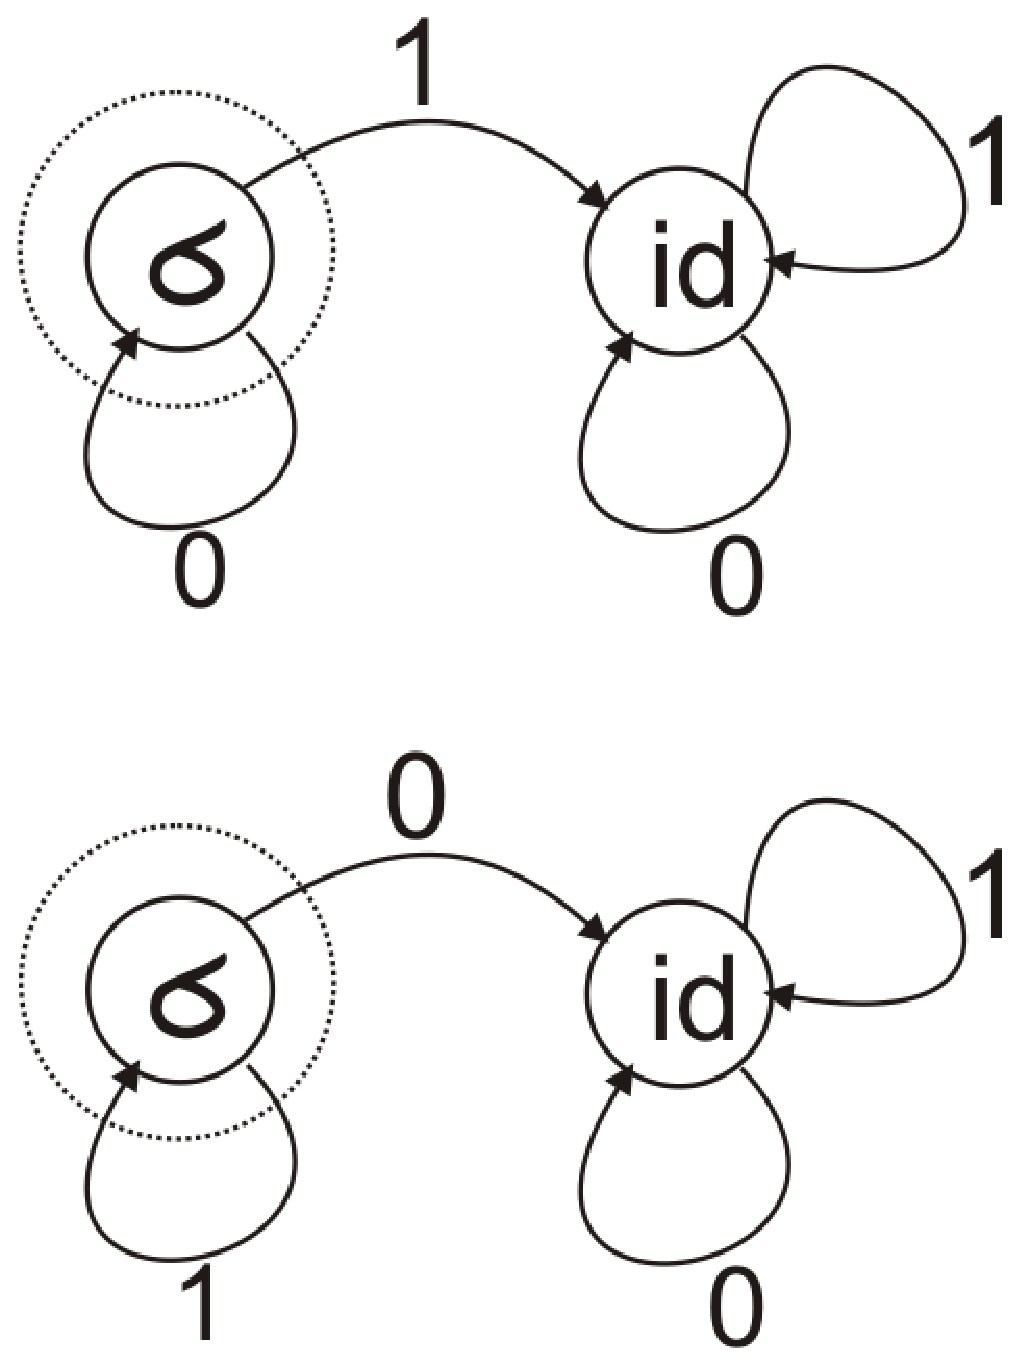
\includegraphics[scale=0.4]{DM.eps}
%\end{center}
 Ототожнюючи кодування елементів простору Бера над двійковим алфавітом з двійковим кодуванням цілих
2-адичних чисел отримаємо представлення автоморфізма функцією на
$Z_2$. Кожен автоморфізм дерева $\alpha$ задає
функцію $f_\alpha$ за правилом: якщо автоморфізм $\alpha$ переводить кінець x в кінець
y, то $f_\alpha(x)=y$. Наприклад $adding \  machine$ при такому представленні
задається функцією $f(x)=x+1$.


Але не кожна функція є автоморфізмом дерева. Для
того, що б функція задавала автоморфізм необхідно, що б ця функція
пару кінців з однаковим початком переводила в пару кінців з
однаковим початком тієї ж самої довжини.
\begin{example}
Функція $f(x)=2x$
переводить пару ...1111 та ...0000 в пару ...1110 та ...0000
відповідно. Перша пара має спільний початок довжини 0, друга  -
довжини 1, тобто функція  $f(x)=2x$ не є автоморфізмом дерева.
\end{example}
\begin{example}
Функція $f(x)=x^2$ не є автоморфізмом дерева.

Дійсно, оскільки має місце наступне співвідношення $$(2^n\cdot t+x)^2=2^{2n}\cdot t^2+2\cdot 2^n\cdot x\cdot
t+x^2$$ тобто $$(2^n\cdot t_1+x)^2-(2^n\cdot t_2+x)^2=$$ $$=(2^{2n}\cdot t_1^2+2\cdot 2^n\cdot x\cdot
t_1+x^2)-(2^{2n}\cdot t_2^2+2\cdot 2^n\cdot x\cdot t_2+x^2)=$$$$= 2^{n+1}(t_2-t_1)(2^{n-1}(t_2+t_1)+1)$$ то для
пари 2-адичних чисел $x_1,x_2$, що мають спільний початок ненульової довжини n, пара $x_1^2,x_2^2$ має спільний
початок довжини як найменше довжини n+1
 отже
відображення $f(x)=x^2$ є неперервним, але не є автоморфізмом.
\end{example}

Втім клас функцій, що є автоморфізмами дерева є досить широким.
Мають місце наступні твердження:
\begin{theorem} \label{st}Функції вигляду
$f(x)=\frac{a^x-1}{a-1}, a=4k+1, k \in Z_2$ є автоморфізмами дерева.
\end{theorem}
\begin{proof}
Функція $f(x)=\frac{a^x-1}{a-1}, a=4k+1, k \in Z_2$ є єдиним розв'язком рівняння $$\chi^{-1}\circ(x+1)\circ\chi=ax+1$$
для якого $$\chi:...000\rightarrow ...000$$.
\end{proof}
 \begin{theorem}Лінійні функції вигляду
$f(x)=ax+b, a=2k+1, a,b,k \in Z_2$ є автоморфізмами дерева.
\end{theorem}


\begin{proof}
Те, що 2-адичні послідовності x та y мають спільний
початок довжини k, рівносильно тому, що послідовність $x-y$ має
наступний вигляд: ...t10...00, де на початку послідовності маємо k
нулів. Але для послідовностей $ax+b$ та $ay+b$  різниця має вигляд
$a(x-y)$, а оскільки а - непарне 2-адичне число, то
$a(x-y)=...t'10...00$, де на початку послідовності маємо k нулів ,
тобто послідовності $ax+b$ та $ay+b$ також мають спільний початок
довжини $k$.
\end{proof}
Добутку автоморфізмів дерева відповідає суперпозиція відповідних функцій.
І для автоморфізмів, і для функцій оберемо ліву дію.
$$\varepsilon^2=\varepsilon\circ \varepsilon=(x+1)\circ (x+1)=(x+1)+1=x+2$$
$$(3x+1)\circ (x+2)=(3x+1)+2=3x+3$$
$$(x+2)\circ (3x+1)=3(x+2)+1=3x+7$$
\begin{lemma}
Для функції $f(x)=ax+b, a=2k+1, a,b,k \in Z_2$ маємо $f^{-1}(x)=\frac{1}{a}(x-b)$.
\end{lemma}
\begin{proof}
$$(ax+b)\circ (\frac{1}{a}(x-b))=\frac{1}{a}((ax+b)-b)=x$$
\end{proof}
Як відомо, операція суперпозиції функцій, взагалі кажучи, не є комутативною. Але для деяких,
 спеціальним способом відібраних функцій комутативність має місце.
\begin{lemma}
Множина функцій $f(x)=x+p\ (p\in Z_2)$ є абелевою групою.
\end{lemma}
\begin{proof}
$$(x+p)^{-1}=x-p$$
$$(x+p_1)\circ(x+p_2)=(x+p_2)\circ(x+p_1)=x+p_1+p_2$$
\end{proof}
\begin{theorem}
Множина лінійних ізометрій кільця $Z_2$ є станово-замкненою самоподібною групою.
\end{theorem}
\begin{proof}
Дійсно, множина станів лінійної функції складається з лінійних функцій:
$$ax=(ax,ax+\frac{a-1}{2}),$$
$$x+2k=(x+k,x+k),$$
$$x+2k+1=(x+k,x+k+1)\circ \sigma,$$
$$ax+2k=ax\circ (x+2k)=(ax,ax+\frac{a-1}{2})\circ (x+k,x+k)=$$ $$=(ax+k,ax+\frac{a-1}{2}+k),$$
$$ax+2k+1=ax\circ (x+2k)=(ax,ax+\frac{a-1}{2})\circ (x+k,x+k+1)\circ \sigma=$$ $$=(ax+k,ax+\frac{a-1}{2}+k+1)\circ \sigma,$$
\end{proof}
добуток лінійних функцій є лінійною функцією:
$$(ax+b)\circ (cx+d)=c(ax+b)+d=cax+(cb+d),$$
та обернена до лінійної функції є лінійною функцією:
$$(ax+b)^{-1}=\frac{1}{a}x-\frac{b}{a}.$$
Нейтральним елементом групи є лінійна функція:
$$f(x)=x.$$
\section{Представлення автоморфізмів регулярного дерева}

\subsection{Портрети автоморфізмів}
%\subsection{Необхідні визначення}

 Автоморфізми зручно задавати портретами. Портретом автоморфізма дерева $T_2$ є дерево $T_2$, вершини якого розмічені 0-ми та 1-ми.

 Автоморфізм задається розміченним деревом в такий спосіб. Якщо автоморфізм переставляє вершини наступного рівня, що суміжні з даною вершиною, то відмітимо цю вершину 1-цею, якщо ні, то 0-лем. Таке представлення автоморфізма назвемо портретом цього автоморфізма.

 При такому представленні автоморфізму $a$ кожному
  кінцю $x$ відповідає послідовність цифр $x_a$ розмічених вершин
   цього кінця, причому кінець
 $x$ під дією автоморфізма $a$ переходить в кінець $x\oplus x_a$
  (під операцією $\oplus$ розуміється покоординатне додавання по модулю 2).


Для опису множення на представленні автоморфізмів дерева портретами знадобляться дві конструкції: додавання портретів за модулем 2 та дія на портрет автоморфізмом дерева.

Множина портретів з операцією додавання за модулем 2 відповідних вершин утворює абелеву групу. Нейтральним елементом цієї групи буде портрет з 0 на всіх вершинах, обернений до елементу групи співпадає з самим елементом.

\begin{center}
\includegraphics[scale=0.7]{SumTr.eps}
\end{center}
Портрет добутку автоморфізмів $a\circ b$ будується наступним чином. Дієм на портрет b автоморфізмом, оберненим до a. Отриманий таким чином новий портрет додаємо по модулю 2 до портрету автоморфізму a.



\begin{center}
\includegraphics[scale=0.4]{MultTree1.eps}
\end{center}

При множенні портретів розмітка кінців дерева змінюється наступним чином:
$$x_{a\circ b}=x_a\oplus (x \oplus x_a)_b$$
Для оберненого до $a$ автоморфізма $a^{-1}$ маємо:
$$(x\oplus x_a)_{a^{-1}}=x_a$$
Наприклад, нехай автоморфізм $a$ задається наступним портретом на дереві $T_2$, на якому виділимо кінець $x$:
\begin{center}
\begin{figure}
\includegraphics[scale=0.20]{ava.eps}
\caption{}
\end{figure}
\end{center}
Згідно з малюнком $$x=...1001$$ $$x_a=...0011$$ тобто $$x\oplus
x_a=...1001\oplus ...0011=...1010$$ і для автоморфізму $a^{-1}$
маємо:$$(x\oplus x_a)_{a^{-1}}=...1010_{a^{-1}}=x_a=...0011.$$
\begin{center}
\includegraphics[scale=0.20]{inva.eps}
\end{center}



Означимо дію $[a]b$ для автоморфізмів a та b з $AutT_2$.
\begin{definition}
Подіємо на розмічене дерево, що задає портрет автоморфізму a автоморфізмом b. Отриманий портрет означимо, як $[a]b$.
\end{definition}
 Для автоморфізмів $a,b,c,d...$ з $AutT_2$ мають місце наступні співвідношення:
$$a \circ b=a \oplus [b]a^{-1}$$
$$[a](b \circ c)=[[a]b]c$$
$$[a\oplus b\oplus c\oplus ...]d=[a]d\oplus [b]d\oplus [c]d\oplus ...$$
Наприклад, має місце рівність:
$$a^{-1}=[a]a.$$
Дійсно: $$a^{-1}\circ a= a^{-1}\oplus [a](a^{-1})^{-1}=a^{-1}\oplus [a]a.$$
З іншого боку $$a^{-1}\circ a=id$$
тобто
$$a^{-1} \oplus [a]a = id$$
$$a^{-1} \oplus [a]a \oplus a^{-1}=id \oplus a^{-1}$$
$$[a]a=a^{-1}.$$
 Аналогічно:

\[
a_n  =  \oplus \sum\limits_{k = 0}^{n - 1} {[a]_{} } a^{ - k}
\]



 Дійсно:
 $$a^n=a\oplus [a^{n-1}]a^{-1}=a\oplus [a\oplus [a^{n-2}]a^{-1}]a^{-1}=$$
 $$=a\oplus [a]a^{-1}\oplus [[a^{n-2}]a^{-1}]a^{-1}=a\oplus [a]a^{-1}\oplus [a^{n-2}]a^{-2}=$$
 $$=a\oplus [a]a^{-1}\oplus...\oplus [a]a^{-k+1} \oplus[a^{n-k}]a^{-k}=a\oplus [a]a^{-1}\oplus...\oplus [a]a^{-n+2} \oplus[a]a^{-n+1}.$$
Опишемо групу скінченностанових автоматних підстановок на мові портретів.
 \begin{definition}Якщо стан автоморфізму діє на піддереві дерева $T_2$, то портрет цього стану є аналогічним піддеревом портрету цього автоморфізму.
 \end{definition}
 Згідно з цім означенням автоморфізм є скінченностановим тоді і тільки тоді, коли множина різних портретів двійкових піддерев дерева $T_2$ є скінченною.

\subsection{Автоматні перетворення}
%\subsection{Необхідні визначення}
Опишемо автомати над алфавітом X.
Автомат складається з алфавіту X, множини станів S, функції переходів $\lambda:S\times X\rightarrow S$ та
 функції виходів $\gamma:S\times X\rightarrow X$. Якщо в стан $s\in S$ попадає елемент $x\in X$, то автомат переходить в стан $\lambda(s,x)$
та повертає елемент $\gamma(s,x)$.

Природнім чином автомат діє на множині послідовностей, що складаються з елементів алфавіту X.
\begin{example}
Означимо автомат з двома станами над алфавітом $\{0,1\}$.
\end{example}
Автомат, що задає автоморфізм дерева зручно записувати у вигляді орієнтованого розміченого графа,
 якій складається з вершин двох типів $\sigma$ та $id$, та множини орієнтованих ребер двох типів,
  помічених 0 та 1, причому з кожної вершини виходить рівно по одному ребру кожного типу.


   Вершини в представленні автомата графом називаються станами автомату. Одна вершина відмічена,
    як ініціальний стан.

    На малюнках наведені автомати:

     для автоморфізму дерева $\varepsilon (adding \ machine)$

    \begin{center}
\includegraphics[scale=0.4]{Auto1.eps}
\end{center}
для автоморфізму $\varepsilon^{-1}$
\begin{center}
\includegraphics[scale=0.4]{Auto2.eps}
\end{center}
та тотожнього автоморфізму $id$
\begin{center}
\includegraphics[scale=0.4]{Autoid.eps}
\end{center}
Автомат діє на кінцях двійкого дерева у такий спосіб.

 Помістимо
першу цифру двійкового розкладу кінця в ініціальний стан автомату.
Якщо цей стан має тип $id$, то автомат повертає цифру, не змінюючи
 її, якщо стан має тип $\sigma$, то  автомат повертає протилежну цифру(0 та 1- протилежні).
 \begin{center}
\includegraphics[scale=0.8]{Autwork.eps}
\end{center}
Добутком $a\circ b$ автоматів a та b називається послідовна дія ціх автоматів.
 Спочатку діємо на послідовність автоматом a, потім автоматом b.
\begin{example}
Добутком автоматів $\varepsilon$ та $\varepsilon^{-1}$ є тотожний автомат $id$:
\begin{center}
\includegraphics[scale=0.8]{MultAutwork.eps}
\end{center}
\end{example}




\subsection{Орієнтовані графи}
%\subsection{Необхідні визначення}


Розглянемо орієнтований граф, вершинами якого є елементи $Z_2$, побудований по автоморфізму a двійкового дерева $T_2$.

Граф будується за наступним правилом: числа x та y з $Z_2$ з'єднані стрілкою, якщо автоморфізм a відповідний кінець $x$ дерева $T_2$ переводить в кінець $y$.

Для автоморфізма $\sigma$,що переставляє вершини 1-го рівня, а на піддеревах, що виходять з цих вершин, діє тотожньо, орієнтовний граф виглядає наступним чином:

\begin{center}
\includegraphics[scale=0.8]{Orsigm.eps}
\end{center}

Для $adding \ machine$ маємо орієнтований граф вигляду:

\begin{center}
\includegraphics[scale=0.4]{Orad.eps}
\end{center}

Для тотожнього автоморфізму $id$ маємо орієнтований граф вигляду:

\begin{center}
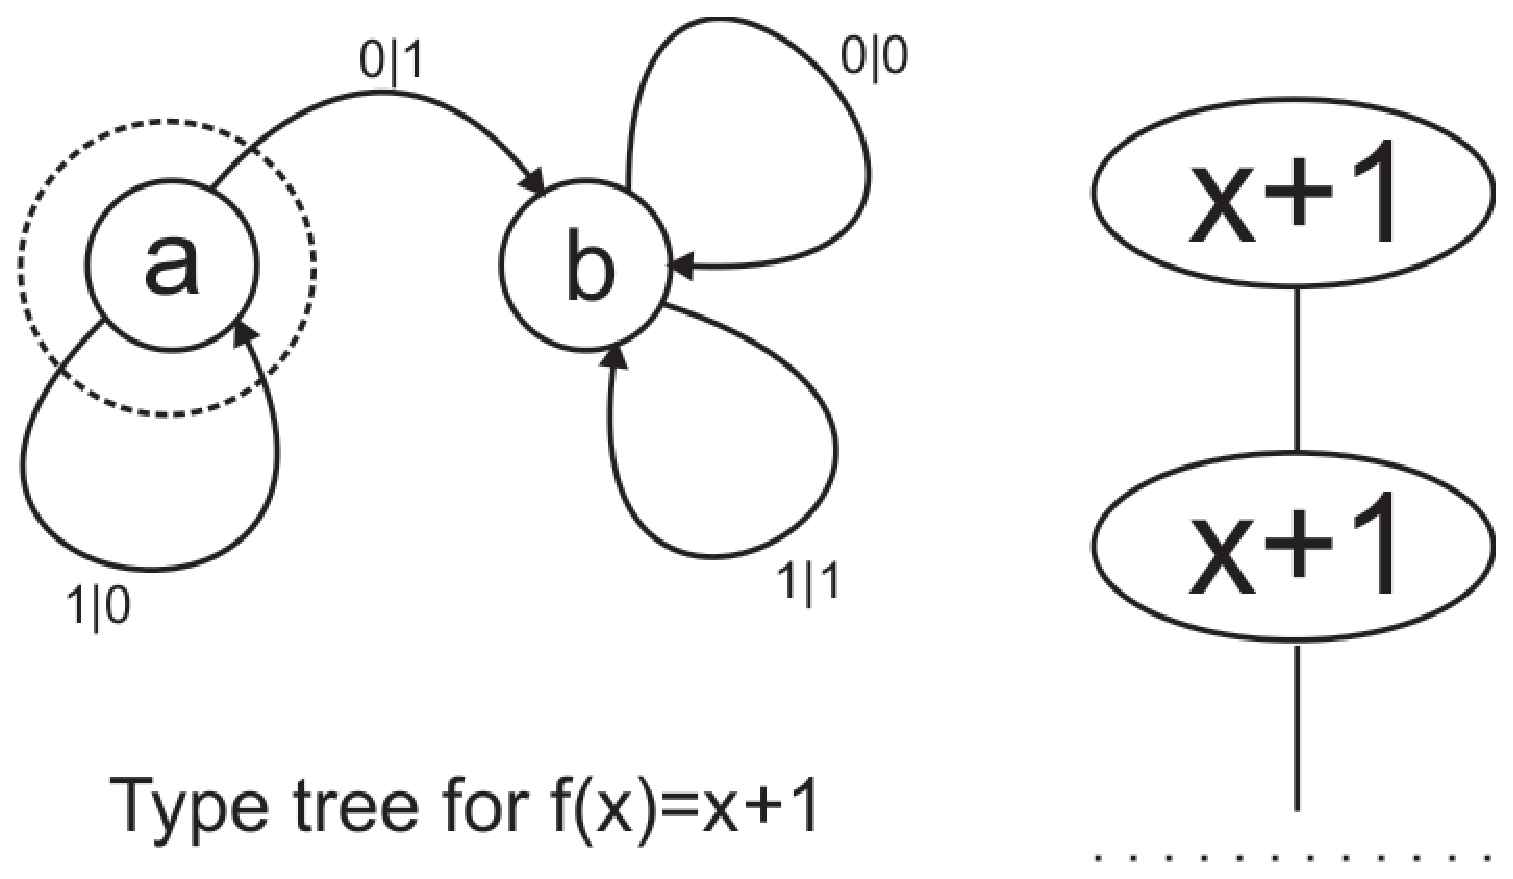
\includegraphics[scale=0.6]{auto_arbas_brbb_1.eps}
\end{center}

 Орієнтований граф автоморфізму природнім чином породжує орієнтовані графи на вершинах, що належать одному рівню.
По орієнтованому графу автоморфізма дерева легко побудувати дерево цикельного типу автоморфізму, яке означається наступним чином: вершинами n-го рівня цього дерева є цикли відповідного орієнтованого графа. Пара вершин дерева типу автоморфізма з'єднана ребром, якщо існує пара суміжних вершин з відповідних ціклів.
\begin{center}
\includegraphics[scale=0.9]{Type_tree1.eps}
\end{center}

Тип автоморфізму відповідає цикловому типу елемента в групі підстановок $S_n$. Побудуємо дерева типу для деяких автоморфізмів.

 Для $adding \ machine$ $\varepsilon$.
  Оскільки на кожному рівні маємо тільки один цикл, то дерево типу є ланцюгом:
\begin{center}
\includegraphics[scale=0.3]{AMgraph.eps}
\end{center}
 Для квадрату $adding \ machine$ $\varepsilon^2$ маємо два цикли, оскільки $$\varepsilon^2=(\varepsilon,\varepsilon)$$
 тобто дерево типу для $\varepsilon^2$ містить два ланцюги:
\begin{center}
\includegraphics[scale=0.6]{Gr(x+2).eps}
\end{center}
Для $f(x)=x\oplus 1$ всі цикли мають довжину 2.

Дійсно, послідовність вигляду $...x_3x_2x_10$ переходить в послідовність вигляду $...x_3x_2x_11$, і навпаки, послідовність вигляду $...x_3x_2x_11$ переходить в послідовність вигляду $...x_3x_2x_10$:
$$...x_3x_2x_10\oplus 1=...x_3x_2x_11$$
$$...x_3x_2x_11\oplus 1=...x_3x_2x_10.$$
 Дерево типу для автоморфізму $f(x)=x\oplus 1$
має вигляд:

\begin{center}
\includegraphics[scale=0.5]{Typesigm.eps}
\end{center}



Для тотожнього автоморфізму $id$,очевидно, всі цикли мають довжину 1, отже дерево типу співпадає з $T_2$:


\begin{center}
\includegraphics[scale=0.5]{Typeid.eps}
\end{center}

\newpage

 \subsection{Матричне представлення}
   В деяких класах задач буває зручно представляти автоморфізми скінченого двійкового n-рівневого дерева матрицями розміру $2^n\times 2^n$.
   Матриця A, що відповідає автоморфізму a будується наступним чином:
  для автоморфізму $a=(b,c)$ матриця A виглядає, як



\[
A = \left( {\begin{array}{*{20}c}
   B & 0  \\
   0 & C  \\
\end{array}} \right)
\]


  для автоморфізму $a=(b,c)\circ \sigma$ матриця A виглядає, як


\[
A = \left( {\begin{array}{*{20}c}
   0 & B  \\
   C & 0  \\
\end{array}} \right)
\]
 де 0- нульова матриця того ж розміру, що матриці B та C.
 Ненульова матриця автоморфізма дерева 0-го рівня( ізольована вершина) записується, як 1-ця.

 За допомогою зворотньої операції по матриці автоморфізма дерева будується портрет цього автоморфізма.



При такому представленні добутку автоморфізмів відповідає добуток матриць:
\begin{center}
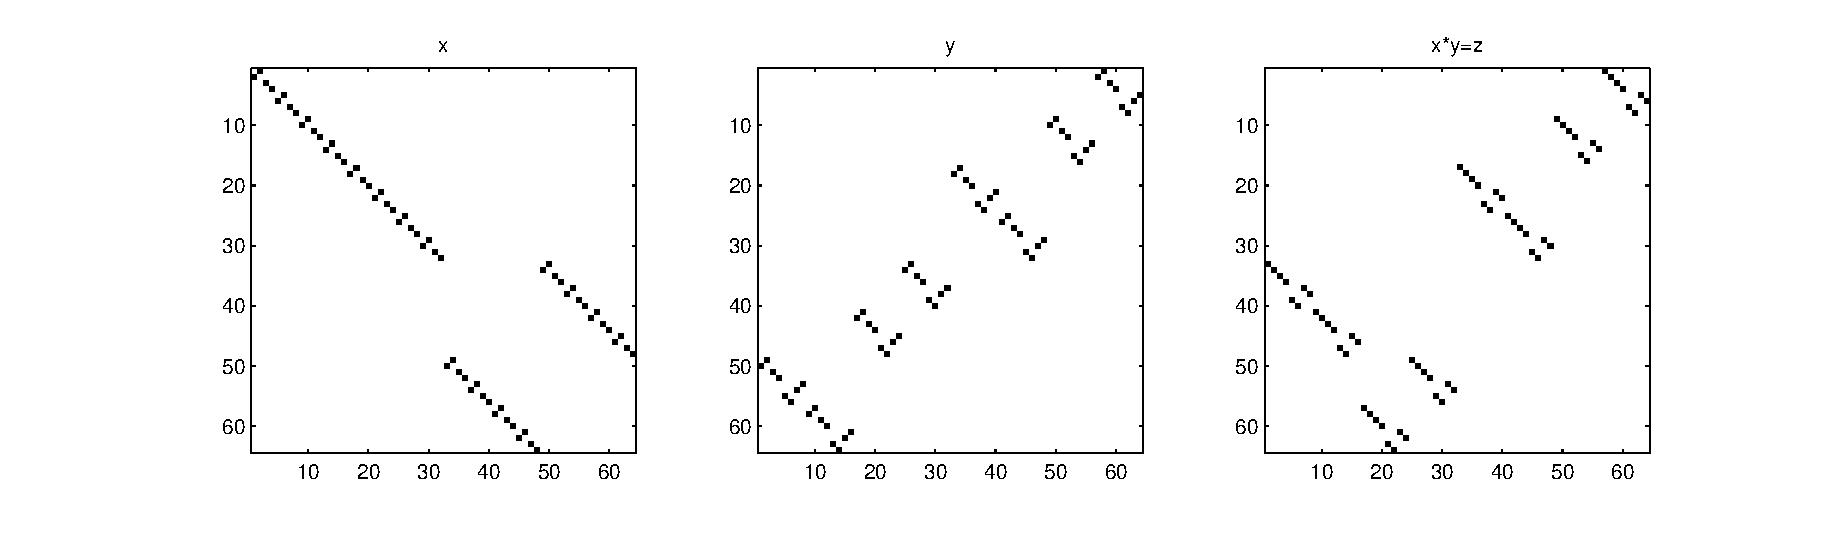
\includegraphics[scale=0.55]{matrprod.eps}
\end{center}
оберненому автоморфізму відповідає обернена матриця:
\begin{center}
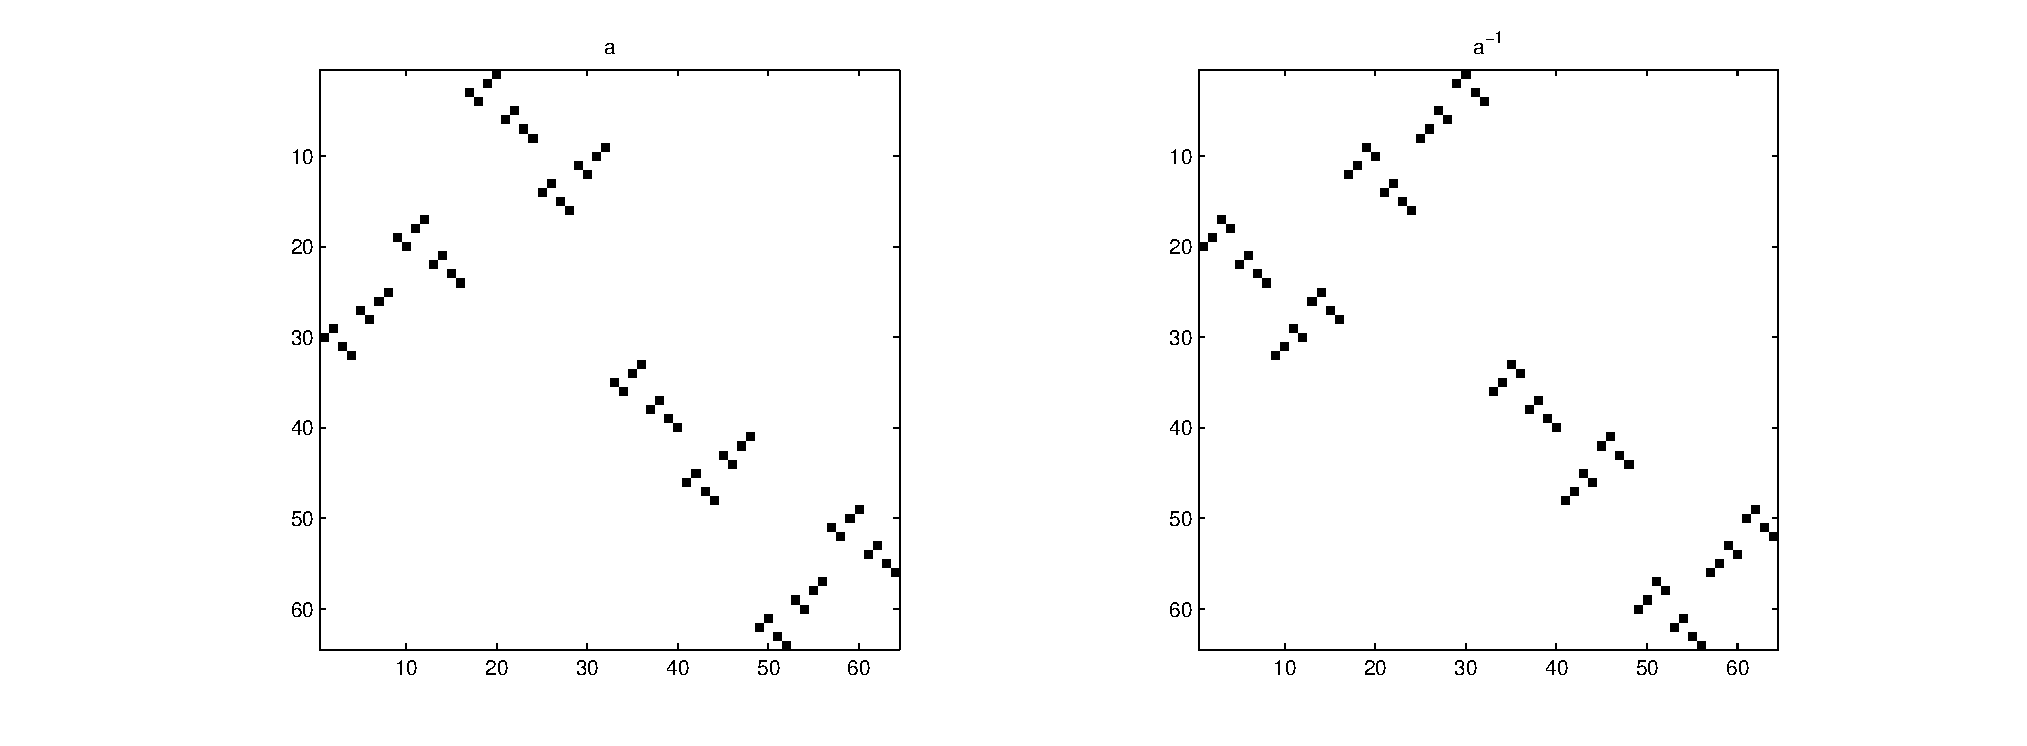
\includegraphics[scale=0.5]{matrinv.eps}
\end{center}
де під крапками розуміються 1-ці.

 Причому для матриці автоморфізма дерева обернена до неї матриця співпадає з транспонованою.

Наприклад епіморфний образ adding machine $\varepsilon_{(7)}$ на дерево з 7-ма рівнями у матричному представленні задається наступною матрицею:
\begin{center}
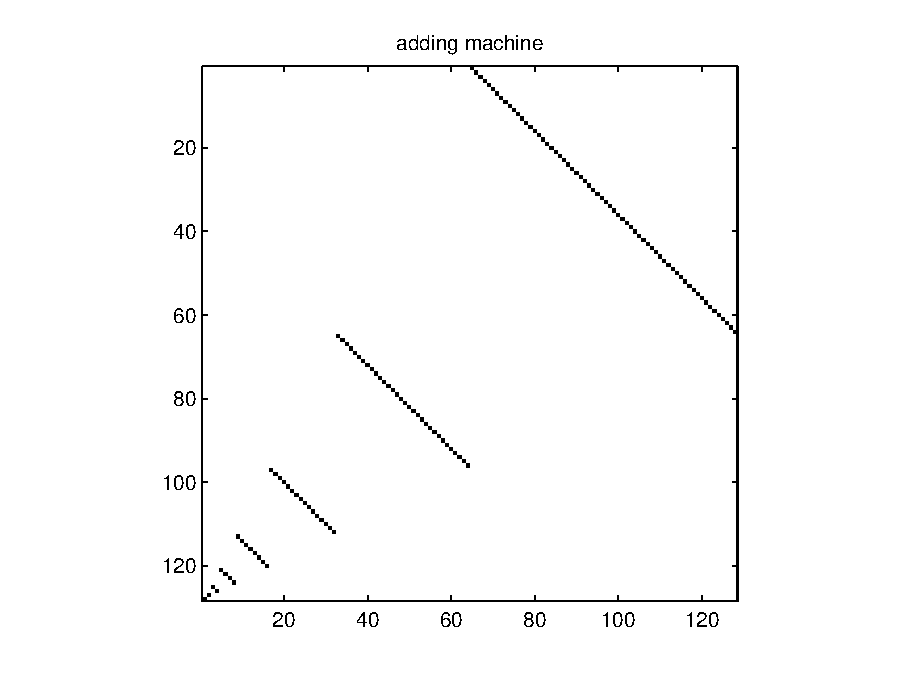
\includegraphics[scale=0.7]{ammatr.eps}
\end{center}


Дійсно, оскільки епіморфний образ adding machine на дерево з 7-ма рівнями задається співвідношенням $\varepsilon_{(7)}=(id_{(6)}),\varepsilon_{(6)}) \circ \sigma$ ( де $\varepsilon_{(7)}$- епіморфний образ adding machine на дерево з 7-ма рівнями, $\varepsilon_{(6)}$- епіморфний образ adding machine на дерево з 6-ма рівнями та $id_{(6)}$- епіморфний образ тотожнього автоморфізму на дерево з 6-ма рівнями), то матриця  для $\varepsilon_{(7)}$ має вигляд:
\[
\varepsilon_{(7)} = \left( {\begin{array}{*{20}c}
   0 & id_{(6)}  \\
   \varepsilon_{(6)} & 0  \\
\end{array}} \right)
\]
 Аналогічно для $\varepsilon_{(6)}$, $\varepsilon_{(5)}$ і т.д.



   Приклад чотирьох  автоморфізмів дерева $(T_2)_5$:
   \begin{center}
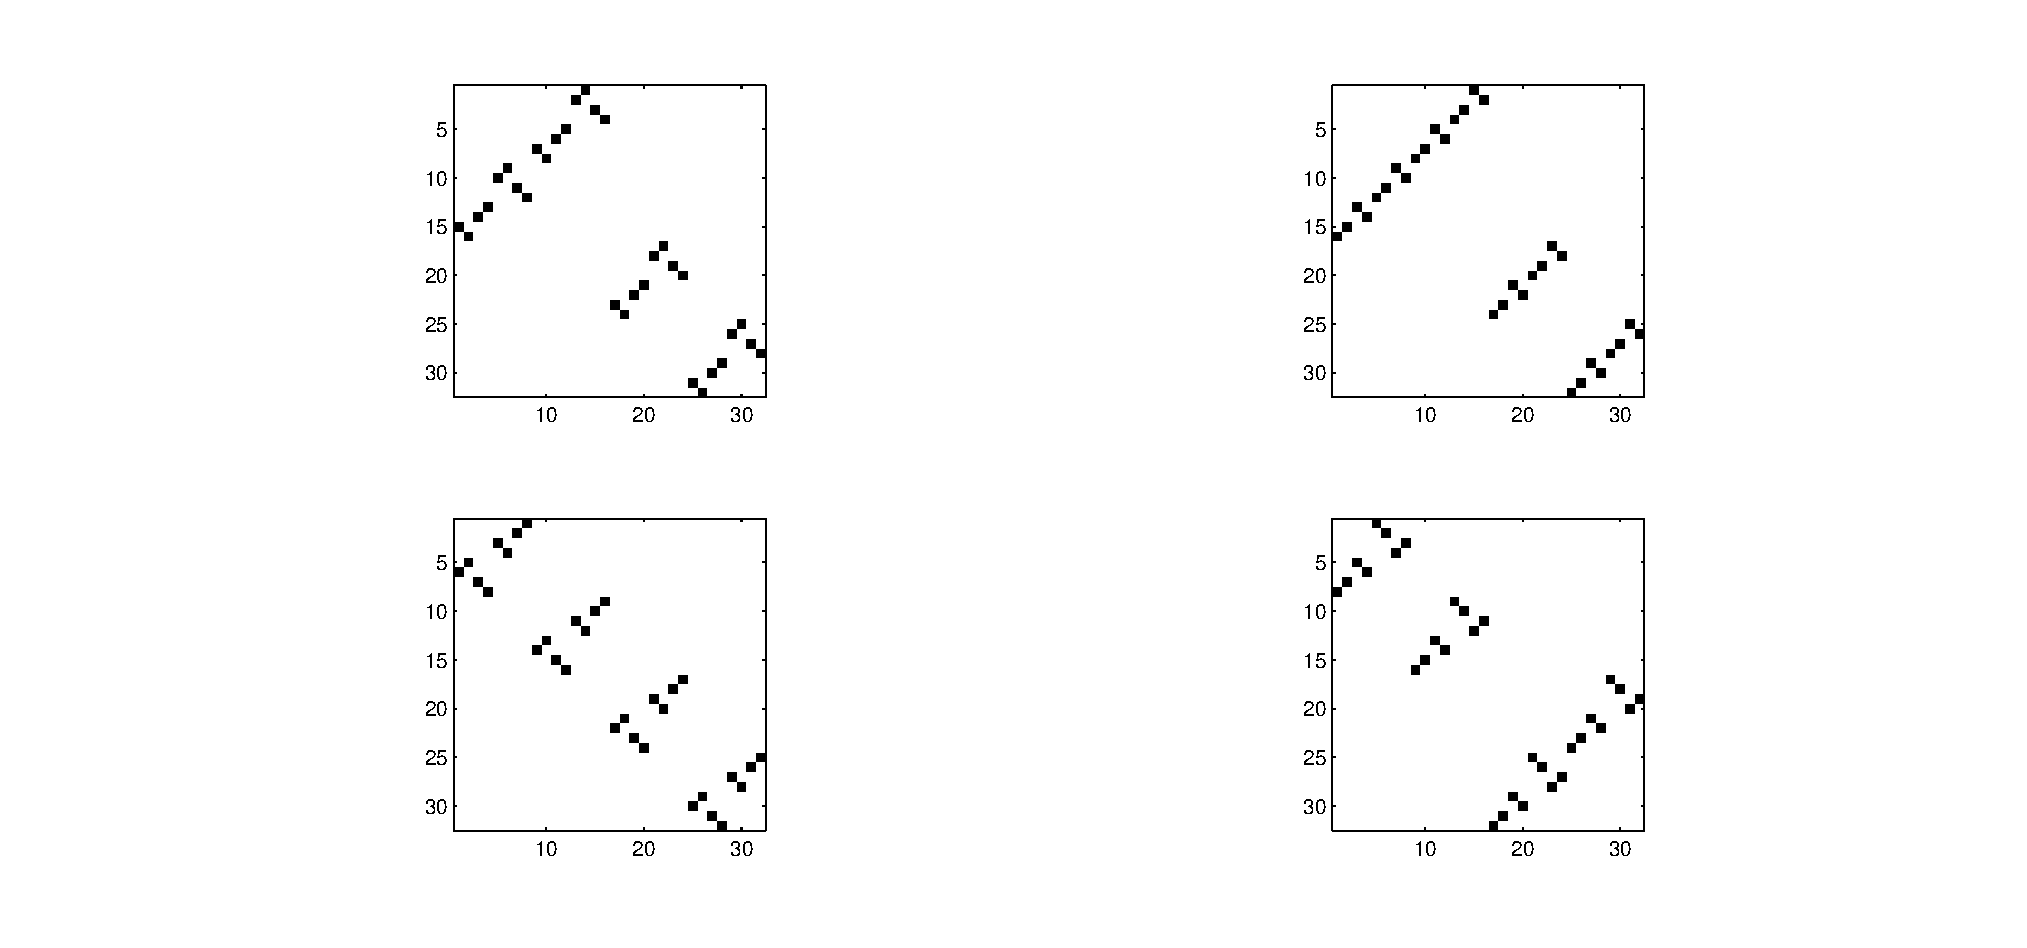
\includegraphics[scale=0.5]{4randm.eps}

\end{center}

Обчислення матриці автоморфізма $f(x)=x-1$, як оберненого до
автоморфізму $f(x)=x+1$:

\begin{center}
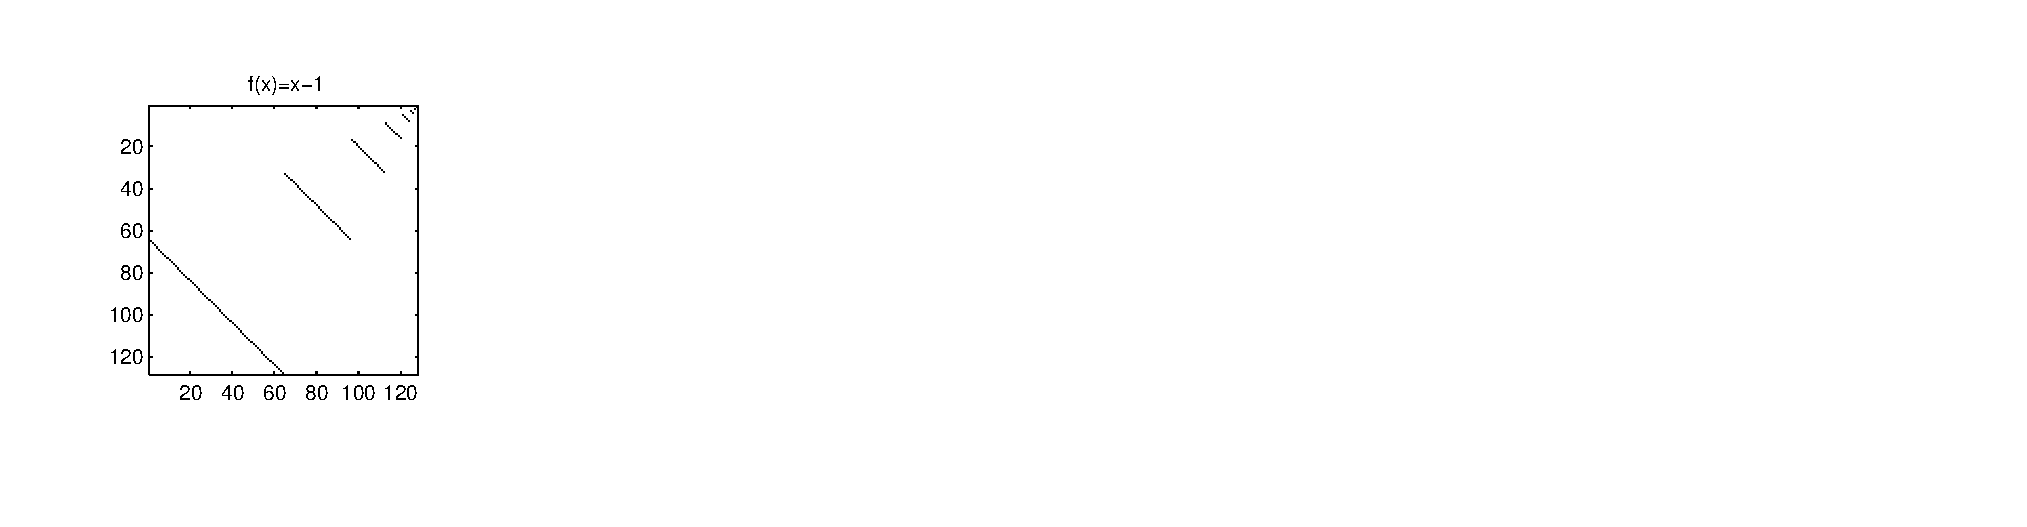
\includegraphics[scale=1.]{mat_x-1.eps}
\end{center}
Обчислення матриці автоморфізма $f(x)=x+k$, як k-го степеня автоморфізма $f(x)=x+1$:

$k=2$
\begin{center}
\includegraphics[scale=0.9]{mat_x+2.eps}
\end{center}
$k=3$
\begin{center}
\includegraphics[scale=0.75]{mat_x+3.eps}
\end{center}
Обчислення матриці автоморфізму $f(x)=ax$, як  розв'язку рівняння $X^{-1}AX=B$, де A - матриця автоморфізму $f(x)=x+1$, B - матриця автоморфізму $f(x)=x+a$:

$a=3$
\begin{center}
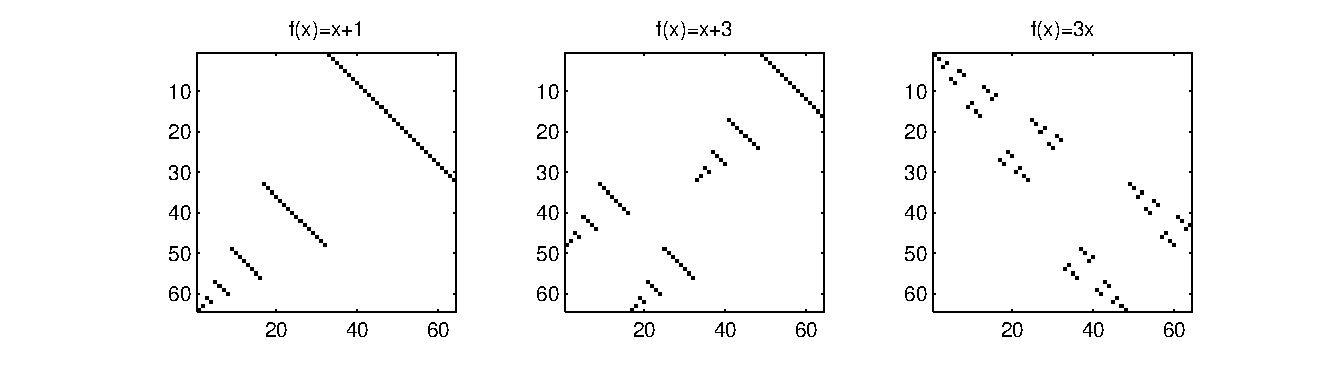
\includegraphics[scale=0.8]{mat_3x.eps}
\end{center}
\bigskip
  Для автоморфізма дерева n-го рівня, що задається матрицею $A$,  будується матриця типу  $A_T=sign(\sum\limits_{k = 1}^{2^n } {A^k })$, за допомогою якої можна побудувати дерево типу для автоморфізму $A$, де $$(sign(A))_{ij}=sign(A_{ij})$$
\[
sign(x) = \left\{ \begin{array}{l}
 0,x = 0 \\
 1,x > 0 \\
 \end{array} \right.
\]


 Обчислимо матриці типу для деяких автоморфізмів.

Для випадкового автоморфізму $A$ дерева $(T_2)_6$:
\begin{center}
\includegraphics[scale=0.5]{matypetree.eps}
\end{center}
Для adding machine:
\begin{center}
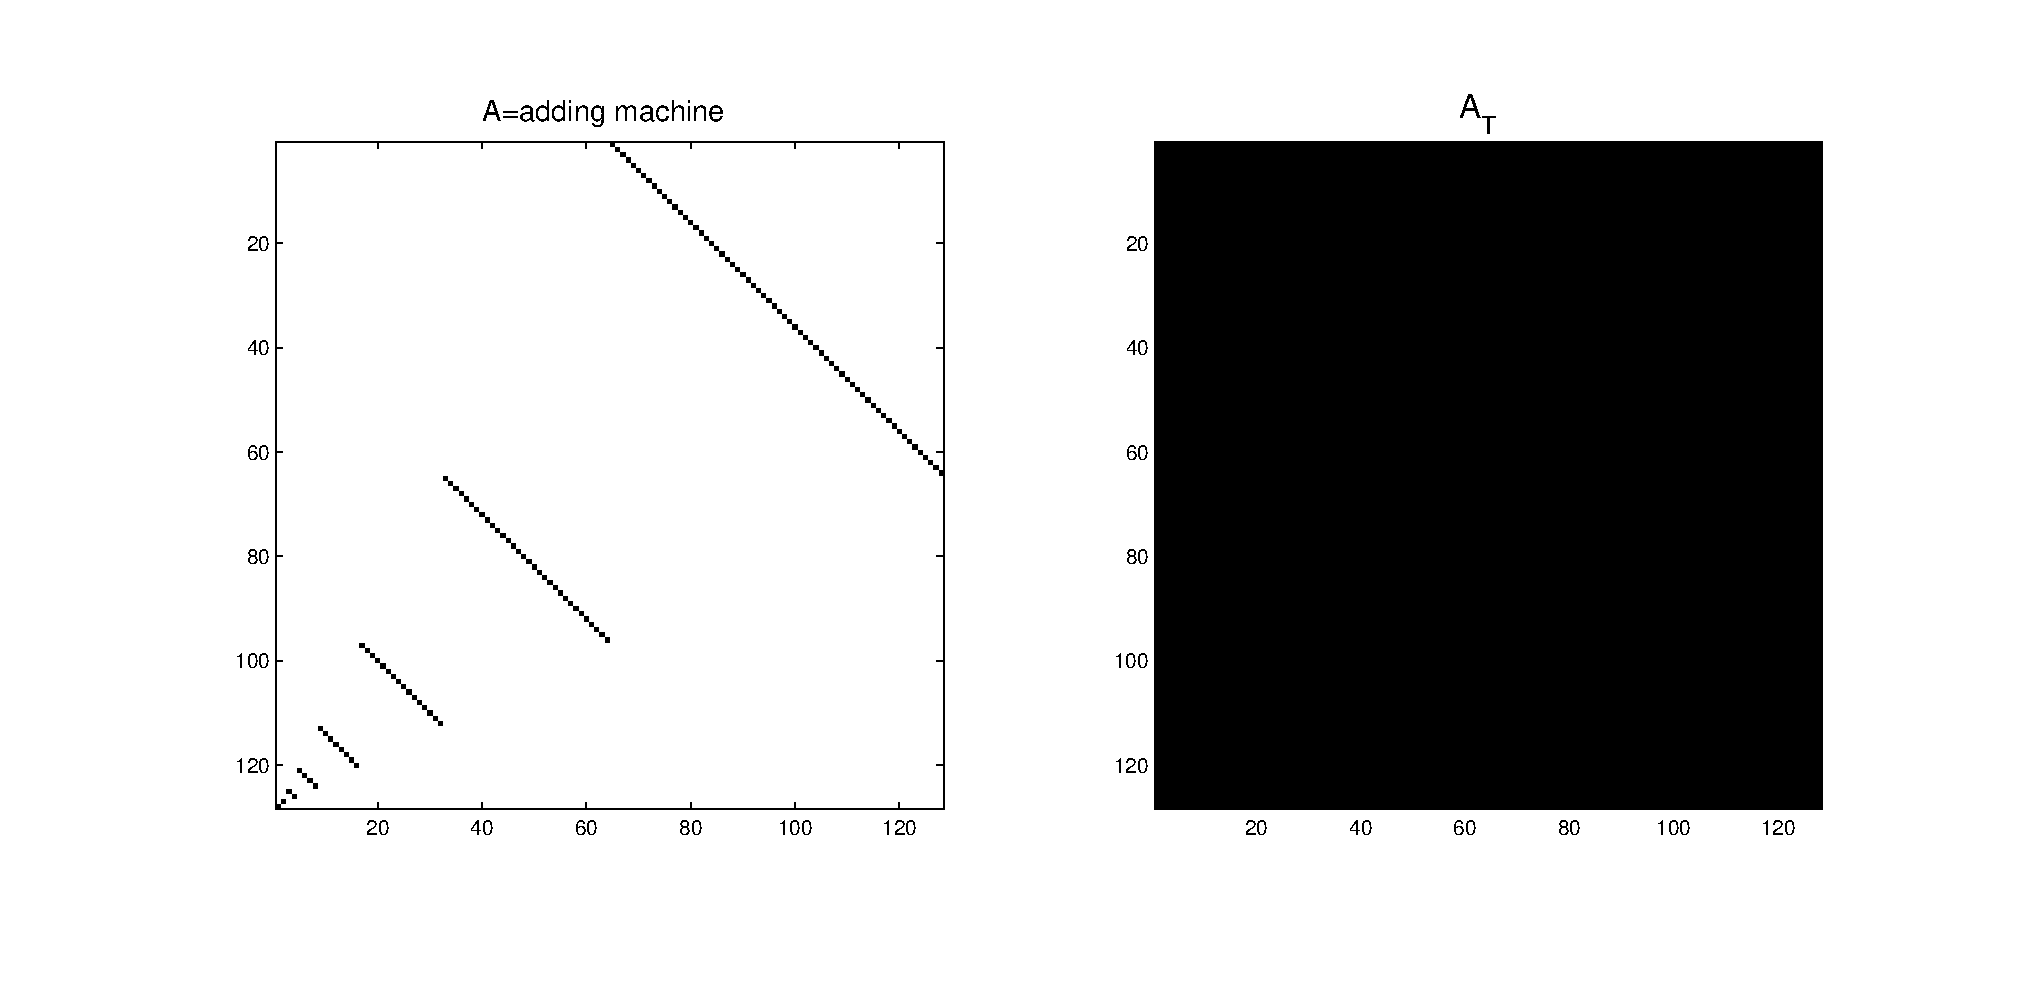
\includegraphics[scale=0.5]{matypetreeAM.eps}
\end{center}
Для $f(x)=3x$:
\begin{center}
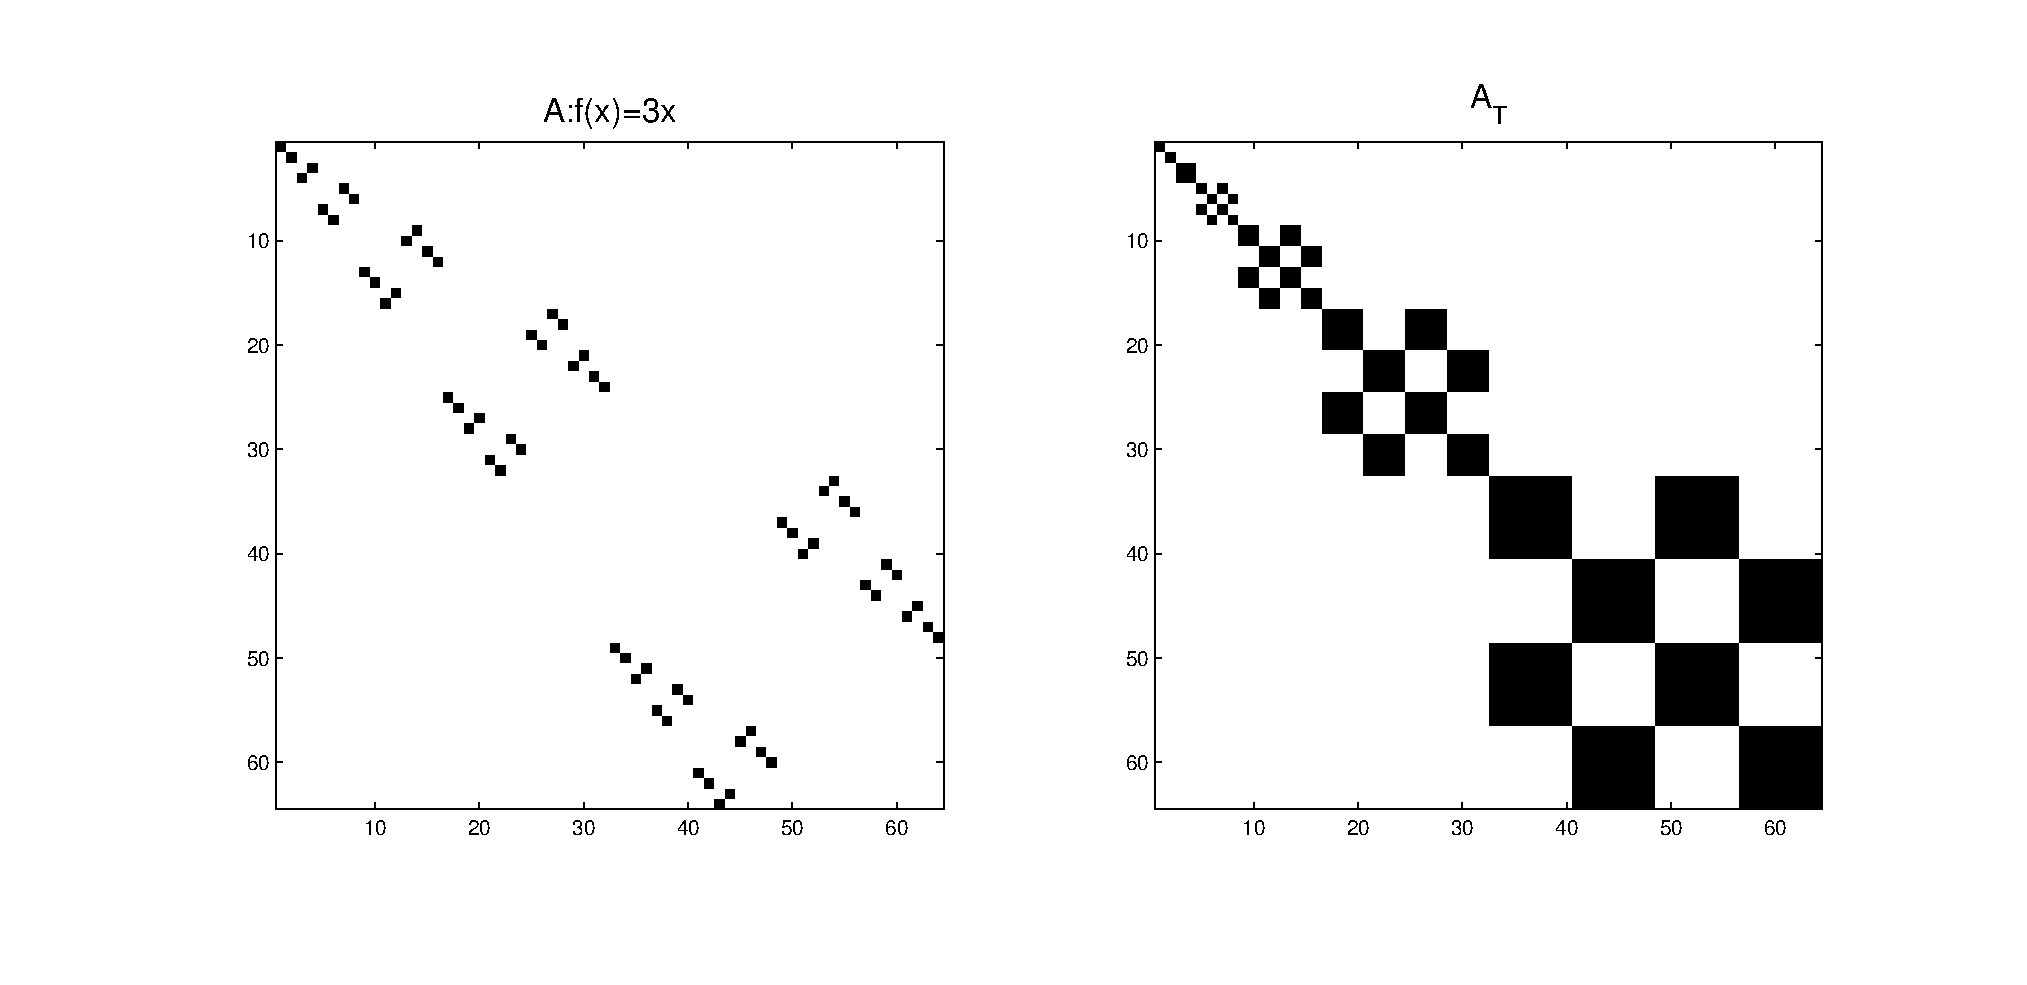
\includegraphics[scale=0.5]{matypetree3x.eps}
\end{center}
Покажемо, як по матриці типу автоморфізму будується дерево типу автоморфізму.

 Очевидно, що якщо $$(A_T)_{kj}=(A_T)_{lj}=1$$ або $$(A_T)_{jk}=(A_T)_{jl}=1$$ для автоморфізму $A$ з $Aut(T_2)_n$ ,
  то кінці $k$ та $l$ належать до однієї орбіти дії $A$ на дереві $(T_2)_n$.

  Далі, для автоморфізма $(A)_n$ дерева $(T_2)_n$, по матриці $(A_T)_n$  побудуємо матрицю $(A_T)_{n-1}$ для автоморфізма $(A)_{n-1}$ дерева $(T_2)_{n-1}$(нагадаємо, що $(A)_n$ - це епіморфний образ автоморфізма $A$ дерева $T_2$ на групу автоморфізмів дерева $(T_2)_n$).

 Означимо функцію $lup(A)$
що діє з множини матриць розміру $2^n\times 2^n$ на множину матриць розміру $2^{n-1}\times 2^{n-1}$:

\[
(lup(A))_{ij}  = \left\{ \begin{array}{l}
 0,\left( {\begin{array}{*{20}c}
   {A_{ij} } & {A_{ij + 1} }  \\
   {A_{i + 1j} } & {A_{i + 1j + 1} }  \\
\end{array}} \right) = \left( {\begin{array}{*{20}c}
   0 & 0  \\
   0 & 0  \\
\end{array}} \right) \\
 1,\left( {\begin{array}{*{20}c}
   {A_{ij} } & {A_{ij + 1} }  \\
   {A_{i + 1j} } & {A_{i + 1j + 1} }  \\
\end{array}} \right) \ne \left( {\begin{array}{*{20}c}
   0 & 0  \\
   0 & 0  \\
\end{array}} \right) \\
 \end{array} \right.
\]
 Приклад послідовної дії функції $lup$ на автоморфізмі adding machine:
 \begin{center}
\includegraphics[scale=0.4]{lupam.eps}
\end{center}
Послідовна дія функції $lup$ на автоморфізмі $f(x)=3x$:
\begin{center}
\includegraphics[scale=0.4]{lup3x.eps}
\end{center}

\begin{lemma}
Мають місце рівності $$(A)_{n-1}=lup((A)_n)$$ $$(A_T)_{n-1}=lup((A_T)_n)$$ $$lup((A_T)_n)=(lup((A)_n))_T$$
\end{lemma}
\begin{proof}
Дійсно, якщо кінці мають спільну вершину $n-1$-го рівня, то їх епіморфні образи на $(T_2)_{n-1}$ співпадають.
\end{proof}

Наприклад, для $A$, що задає автоморфізм дерева $T_2$ $f(x)=3x$, маємо наступну матрицю типу $A_T$( $A_T$ вказана разом з $A$):
\begin{center}
\includegraphics[scale=0.4]{taa3x.eps}
\end{center}

Послідовно застосовуючи до неї функцію lup отримуємо матриці типу для епіморфних образів автоморфізму $f(x)=3x$ на $Aut(T_2)_n$ $(1\leq n\leq 6)$:
\begin{center}
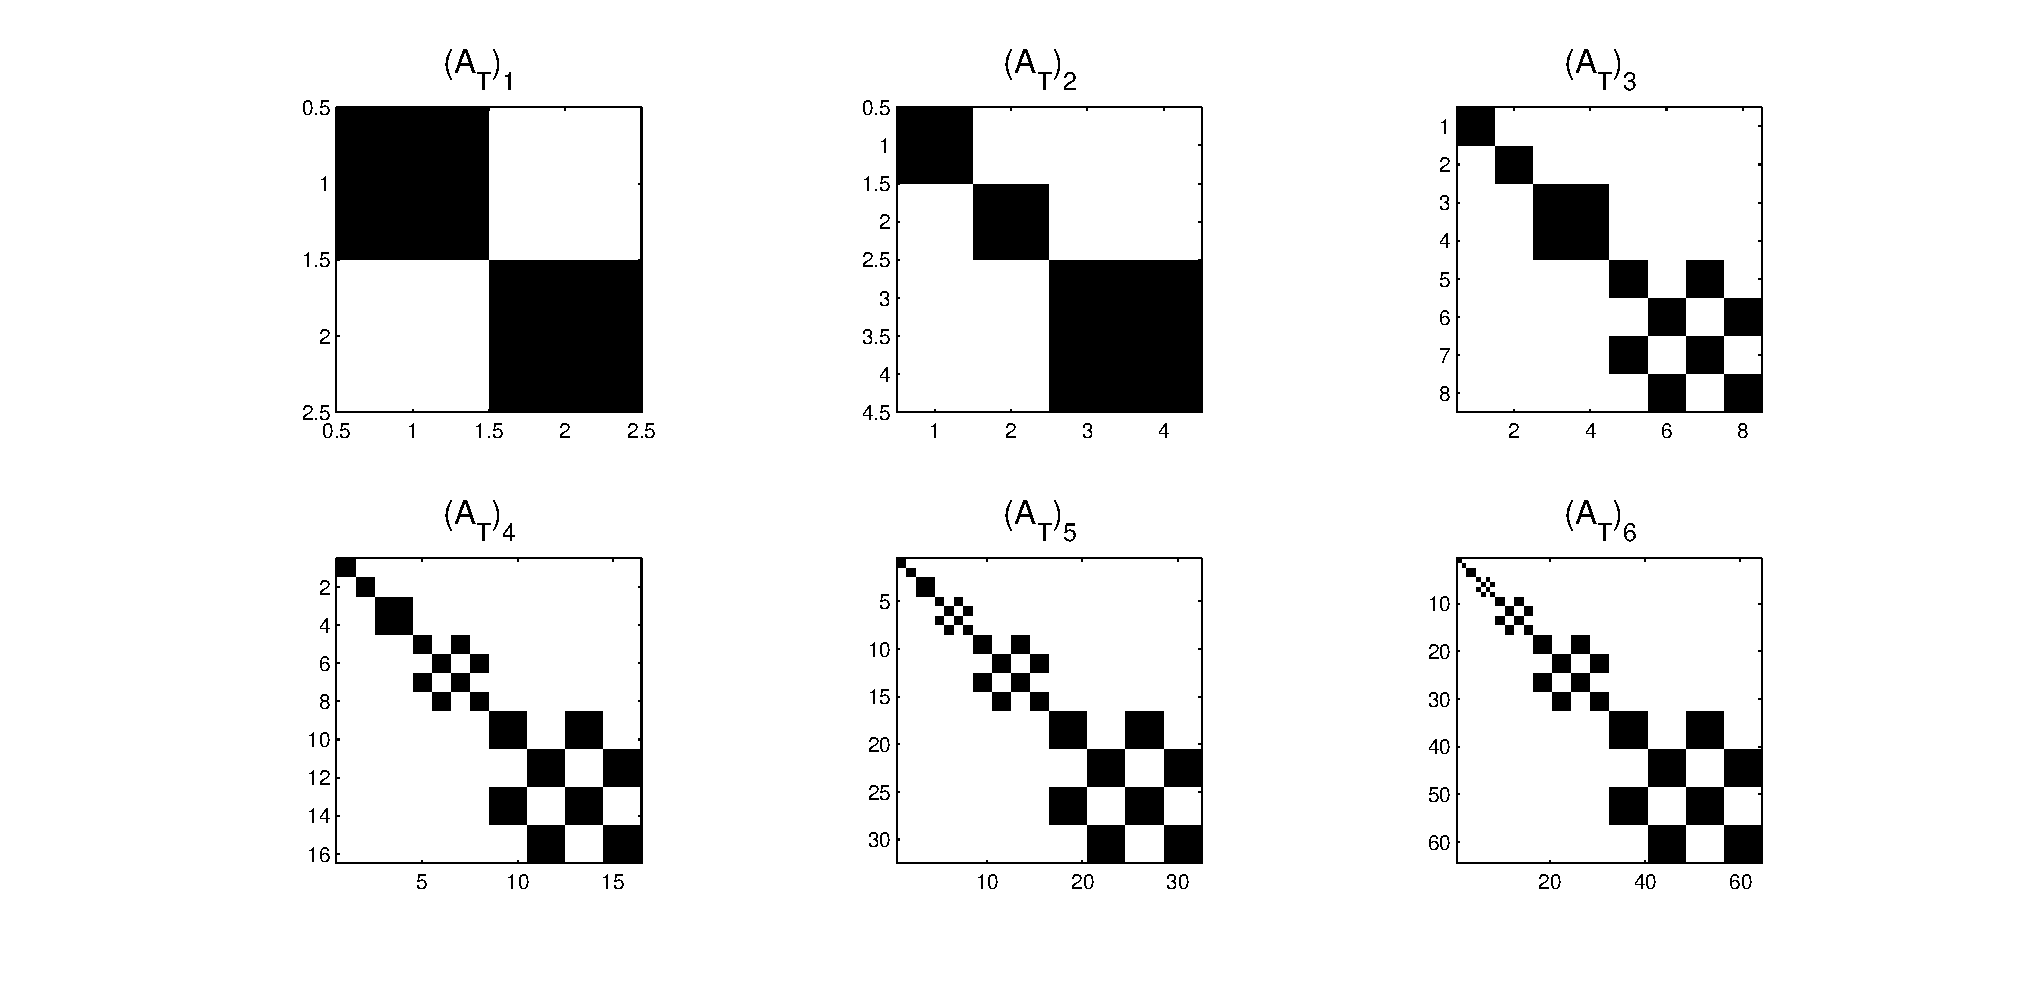
\includegraphics[scale=0.5]{evmatypetr3x.eps}
\end{center}
Згідно з $(A_T)_1$ дія $A$ на $(T_2)_1$ має дві орбіти, тобто дерево типу автоморфізму $A$ має дві вершини на 1-му рівні.

%  :
% \begin{center}
% \includegraphics[scale=0.6]{buildttst1.eps}
% \end{center}
Далі, згідно з $(A_T)_2$ для дії $A$ на $(T_2)_2$  одна з орбіт ділиться на дві орбіти 2-го рівня, тобто маємо три орбіти 2-го рівня:
\begin{center}
\includegraphics[scale=0.6]{buildttst2.eps}
\end{center}
Аналогічно отримаємо 3-тій рівень дерева типу:
\begin{center}
\includegraphics[scale=0.6]{buildttst3.eps}
\end{center}
Продовжуючи побудову  отримаємо самоподібне дерево типу для автоморфізму $A$:
\begin{center}
\includegraphics[scale=0.5]{buildttstf.eps}
\end{center}
\subsection{Зв'язок між  представленнями}
%\subsection{Необхідні визначення}
 Опишемо зв'язок між  представленнями, побудованими в попередніх розділах.
  На малюнку маємо представлення adding machine у п'яти вищезгаданих мовах:

\begin{center}
\includegraphics[scale=0.8]{5mov.eps}
\end{center}

Побудуємо по функції $f(x)=3x$ її алгебраїчний запис.

Подіємо на 2-адичні послідовністі $ x0$ та $x1$ функцією $f$(де x - це 2-адичний розклад числа x).
$$x0=2x$$ $$ 3(x0)=3(2x)=2(3x)=(3x)0$$
$$x1=2x+1$$ $$ 3(x1)=3(2x+1)=2(3x+1)+1=(3x+1)1$$
Тобто $$3x=(3x,3x+1).$$

За допомогою алгебраїчного запису представимо автоморфізми у автоматному вигляді.
Для $adding \  machine$ $$x+1=(id,x+1)\circ \sigma$$ тобто маємо 2-становий автомат:

 \begin{center}
\includegraphics[scale=0.8]{alg_to_auto.eps}
\end{center}
Для функції $f(x)=3x$
$$3x=(3x,3x+1)$$
$$3x+1=3x\circ (x+1)=(3x,3x+1)\circ (id,x+1)\circ \sigma=(3x,3x+2)\circ \sigma$$
$$3x+2=3x\circ (x+2)=(3x,3x+1)\circ (x+1,x+1)=(3x+1,3x+2)\circ \sigma$$
Маємо 3 стани $3x,3x+1$ та $3x+2$.

 Стани $3x$ та $3x+2$ мають тип $id$, стан $3x+1$ має тип $\sigma$:

\begin{center}
\includegraphics[scale=0.8]{3x.eps}
\end{center}

 Змінюючи ініціальний стан отримуємо автомати для функцій $f(x)=3x+1$ та $f(x)=3x+2$:


 \begin{center}
\includegraphics[scale=0.8]{3x+1.eps}
\end{center}
\begin{center}
\includegraphics[scale=0.8]{3x+2.eps}
\end{center}
5-становий автоморфізм, що задається функцією $f(x)=5x$ визначається наступними співвідношеннями:
 $$a_0=(a_0,a_2)$$
 $$a_1=(a_0,a_3)\circ\sigma$$
$$a_3=(a_1,a_4)\circ\sigma$$
$$a_2=(a_1,a_3)$$
$$a_4=(a_2,a_4)$$
з ініціальним станом $a_0$.
\begin{center}
\includegraphics[scale=0.23]{avt5x.eps}
\end{center}
Змінюючи ініціальний стан отримуємо автомати для функцій $f(x)=5x+1$
\begin{center}
\includegraphics[scale=0.20]{avt5x1.eps}
\end{center}
$f(x)=5x+2$
\begin{center}
\includegraphics[scale=0.20]{avt5x2.eps}
\end{center}
$f(x)=5x+3$
\begin{center}
\includegraphics[scale=0.20]{avt5x3.eps}
\end{center}
та $f(x)=5x+$
\begin{center}
\includegraphics[scale=0.20]{avt5x4.eps}
\end{center}
 Покажемо, як по автомату будується портрет автоморфізму.

 Автомат з початковим ініціальним станом задає автоморфізм двійкового дерева. З початкового ініціального стану виходять дві
стрілки, помічені 0 та 1, кінцями яких є стани $a_0$ та $a_1$ відповідно.

Автомат з початковим станом $a_0$ задає дію на ліве піддерево, автомат з початковим станом $a_1$ задає дію на праве піддерево, і т.д.
Наприклад, для автоморфізму $f(x)=3x$ маємо:
$$3x=(3x,3x+1)$$
$$3x+1=(3x,3x+2)\circ\sigma$$
$$3x+2=(3x+1,3x+2)$$
\begin{center}
\includegraphics[scale=0.15]{portst3x.eps}
\end{center}

Приймаючи до уваги, що автоморфізм $f(x)=3x+1$ переставляє вершини першого рівня дерева $T_2$ ,
 а автоморфізми $f(x)=3x$ та $f(x)=3x+2$ залишають на місці вершини першого рівня,
отримуємо портрет для автоморфізму $f(x)=3x$:

\begin{center}
\includegraphics[scale=0.16]{port3x.eps}
\end{center}

По функціональному представленню автоморфізму $a$ $$a:x\rightarrow f(x)$$
побудуємо орієнтований граф. Кожен цикл цього графа буде мати вигляд
$$...\rightarrow f^{-1}(x^{(1)}_0)\rightarrow f^0(x^{(1)}_0)\rightarrow f^1(x^{(1)}_0)\rightarrow f^2(x^{(1)}_0)...$$
$$...\rightarrow f^{-1}(x^{(2)}_0)\rightarrow f^0(x^{(2)}_0)\rightarrow f^1(x^{(2)}_0)\rightarrow f^2(x^{(2)}_0)...$$
$$...................$$
 $$...\rightarrow f^{-1}(x^{(k)}_0)\rightarrow f^0(x^{(k)}_0)\rightarrow f^1(x^{(k)}_0)\rightarrow f^2(x^{(k)}_0)...$$
 $$...................$$
  де кінці $x^{(k_1)}_0$ та $x^{(k_2)}_0$ для $k_1\neq k_2$ належать різним циклам,
   тобто не існує $p\in Z_2$, такого, що $$f^p(x^{(k_1)}_0)=x^{(k_2)}_0$$
   Наприклад, для автоморфізма вигляду $f(x)=5x+1$ маємо єдиний цикл вигляду:
   $$...\rightarrow -\frac{1}{5}\rightarrow 0\rightarrow 1\rightarrow 6\rightarrow 31\rightarrow 0...$$
Це представлення зручно використовувати для знаходження $\chi$ в рівнянні спряженості $$\chi^{-1}\circ a \circ \chi= b.$$
Наприклад, якщо автоморфізми a та b в  представленні орієнтованими графами мають єдиний цикл:
$$a=...\rightarrow f^{-1}(x^{(a)}_0)\rightarrow f^0(x^{(a)}_0)\rightarrow f^1(x^{(a)}_0)\rightarrow f^2(x^{(a)}_0)... ,$$
$$b=...\rightarrow f^{-1}(x^{(b)}_0)\rightarrow f^0(x^{(b)}_0)\rightarrow f^1(x^{(b)}_0)\rightarrow f^2(x^{(b)}_0)... ,$$
то автоморфізм $\chi$ задається наступним чином:
$$f^{-1}(x^{(a)}_0)\rightarrow f^{-1}(x^{(b)}_0)$$
$$x^{(a)}_0\rightarrow x^{(b)}_0$$
$$f(x^{(a)}_0)\rightarrow f(x^{(b)}_0)$$
$$................$$
$$f^{k}(x^{(a)}_0)\rightarrow f^{k}(x^{(b)}_0),\forall k \in Z_2. $$
Покладемо $a(x)=x+1,b(x)=x+3$.
Для автоморфізмів a та b в  представленні орієнтованими графами маємо по одному циклу наступного вигляду:
$$a=...\rightarrow -1 \rightarrow 0 \rightarrow 1 \rightarrow 2 \rightarrow 3 ... ,$$
$$b=...\rightarrow -3 \rightarrow 0 \rightarrow 3\rightarrow 6 \rightarrow 9 ... .$$
Тобто автоморфізм $\chi$ задається наступним чином:
$$-1 \rightarrow-3$$
$$0 \rightarrow 0$$
$$1 \rightarrow 3$$
$$................$$
$$k \rightarrow 3k, \forall k \in Z_2. $$
З цього отримуємо, що у представленні автоморфізмів 2-адичними функціями $\chi(x)=3x$. Дійсно:
 $$(3x)^{-1}\circ (x+1)\circ 3x= \frac{1}{3}x\circ (x+1)\circ 3x =$$$$=(\frac{1}{3}x+1)\circ 3x=3(\frac{1}{3}x+1)=x+3.$$
Побудова по портрету матриці.


Нехай автоморфізм $a\in AutT_2$ задано портретом:
\begin{center}
\includegraphics[scale=0.7]{Autfm.eps}
\end{center}
Користуючись правилом, що автоморфізму a, що задається співвідношенням $a=(b,c)\circ \sigma$
 відповідаєbпортрет
\begin{center}
\includegraphics[scale=0.3]{port1ab.eps}
\end{center}
та матриця
\[
\left( {\begin{array}{*{20}c}
   0 & B  \\
   C & 0  \\
\end{array}} \right)
\]
а автоморфізму, що задається співвідношенням $a=(b,c)$ відповідає портрет

\begin{center}
\includegraphics[scale=0.3]{port0ab.eps}
\end{center}
та матриця
\[
\left( {\begin{array}{*{20}c}
   B & 0  \\
   0 & C  \\
\end{array}} \right)
\]
отримаємо наступну послідовність кроків побудови матриці автоморфізму:
1-й крок
\begin{center}
\includegraphics[scale=0.4]{Autfm4.eps}
\end{center}
2-й крок
\begin{center}
\includegraphics[scale=0.6]{Autfm3.eps}
\end{center}
3-й крок
\begin{center}
\includegraphics[scale=0.5]{Autfm2.eps}
\end{center}
Продовжуючи цю процедуру до n-го кроку отримаємо матричне представлення для епіморфного образу автоморфізма на $(AutT_2)_n$.

Побудова по матриці портрету.

Побудуємо портрет автоморфізму a по його матриці A:
\begin{center}
\includegraphics[scale=0.3]{m2p.eps}
\end{center}
 Оскільки матриці
\[
\left( {\begin{array}{*{20}c}
   B & 0  \\
   0 & C  \\
\end{array}} \right)
\]
відповідає портрет
 \begin{center}
\includegraphics[scale=0.25]{port0ab.eps}
\end{center}

 а матриці
\[
\left( {\begin{array}{*{20}c}
   0 & B  \\
   C & 0  \\
\end{array}} \right)
\]
портрет
\begin{center}
\includegraphics[scale=0.25]{port1ab.eps}
\end{center}
то побудова портрету зводиться до послідовного використання функції, оберненої до $lup$.


Застосувавши функцію lup до матриці автомрфізму A чотири рази отримаємо:
\begin{center}
\includegraphics[scale=0.5]{m2ptype.eps}
\end{center}
$lup^{(4)}(A)$ повертає матрицю
 \begin{center}
\includegraphics[scale=0.55]{m2p4.eps}
\end{center}
 портрет для якої має вигляд
 \begin{center}
\includegraphics[scale=0.3]{port1ab.eps}
\end{center}
Застосуємо цю операцію послідовно для:

 $lup^{(4)}(A)$
\begin{center}
\includegraphics[scale=0.6]{m2plup1.eps}
\end{center}
$lup^{(3)}(A)$
\begin{center}
\includegraphics[scale=0.4]{m2plup2.eps}
\end{center}
$lup^{(2)}(A)$
\begin{center}
\includegraphics[scale=0.4]{m2plup3.eps}
\end{center}
і остаточно маємо портрет для автоморфізму a, побудований по матриці A:
\begin{center}
\includegraphics[scale=0.4]{m2plup4.eps}
\end{center}
\bigskip
\newpage



\section{Централізатори}
\subsection{Cпряженість в $AutT_2$}
Два елемента $a$ та $b$ групи $G$ називають спряженими в цій групі,
 якщо існує розв'язок $\chi$ рівняння $$\chi^{-1}\circ a\circ \chi=b$$ такий, що $\chi \in G$.

 Рядок $\chi^{-1}\circ a\circ \chi$ часто записують, як $a^\chi$.

 Розв'язки рівняння $a^\chi=a$ утворюють підгруппу групи $G$, яка називається централізатором елемента в цій групі
 і позначається, як $C_G(a)$.


 Опис централізаторів є важливим при дослідженні питання спряженості,
  оскільки усі розв'язки рівняння $a^\chi =b$ мають вигляд $\chi=C_G(a) \circ \chi_0$, де $\chi_0$- частковий розв'язок цього рівняння.
  \begin{definition}
  Шарово-однорідним назвемо автоморфізм, для якого дерево типу є ланцюгом.
\end{definition}
Для шарово-однорідного автоморфізму $a$ означимо $a^{k}, k\in Z_2$.


Для $adding\ machine$ $\varepsilon$ означимо $\varepsilon^k$, як елемент централізатора $C_{AutT_2}(\varepsilon)$,
 який $...000$ переводить в $k$.
 $$\varepsilon^k:=\chi_k$$
 де
 $$\varepsilon^{\chi_k}=\varepsilon$$
 $$\chi_k:...000\rightarrow k$$

 Нехай $\chi_a$ частковий розв'язок рівняння $\varepsilon^{\chi}=a$.
 Означимо $a^k$ для $k \in Z_2$:
 $$a^k:=(\varepsilon^k)^{\chi_a}.$$
 Для цілих $k$ означення співпадає зі звичайним піднесенням у степінь.

Питання про те, чи спряжені два автоморфізми дерева в  $AutT_n$ є повністю розв'язанним(роботи). Має місце наступне твердження.
 \begin{theorem}
Автоморфізми дерева спряжені в $AutT_n$, тоді і тільки тоді, коли їх дерева типу ізоморфні.
\end{theorem}
Наприклад, автоморфізми $f(x)=x+2$ та $f(x)=(x+1,x-1)$ спряжені в $AutT_2$, так як мають ізоморфні дерева типу.
\begin{center}
\includegraphics[scale=0.25]{conj1.eps}
\end{center}

Розв'язок $\chi_0$ рівняння $a^\chi=b$, що переводить кінець $x_0$ в кінець $y_0$, для шарово-однорідних
автоморфізмів $a$ та $b$
  описується наступним чином:
$$\chi_0:x_k\rightarrow y_k$$ де $$x_k=(x_0)a^k,\  y_k=(y_0)a^k\  (k\in Z_2)$$
\begin{center}
\includegraphics[scale=0.5]{conjab.eps}
\end{center}
 Як приклад побудуємо розв'язок $\chi_0$ рівняння $$(x+1)^{\chi}=x+p$$ такий, що $\chi_0:...000\rightarrow ...000$:
 \begin{center}
\includegraphics[scale=0.5]{conj1p.eps}
\end{center}
Дійсно $$px:...000\rightarrow ...000$$
 $$(x+1)^{px}=\frac{1}{p}x\circ (x+1)\circ px=p(\frac{1}{p}x+1)=x+p$$
 Побудуємо розв'язок $\chi_0$ рівняння $$(5x+1)^{\chi}=25x+1$$ такий, що $\chi_0:...000\rightarrow ...000$.
  Автоморфізми $f(x)=5x+1$ та $f(x)=25x+1$ - шарово-однорідні, отже спряжені, і маємо по одному циклу.
 Для шарово-однорідного автоморфізму пронумеруємо елементи циклу: елементом номеру p назвемо кінець x дерева $T_2$, для якого $$x=...000*a^p.$$
  Елементом номеру p для автоморфізму $f(x)=5x+1$ є $\frac{5^p-1}{4}$.

 Елементом номеру p для автоморфізму $f(x)=25x+1$ є $\frac{25^p-1}{24}$.

 Тобто автоморфізм $\chi_0$ переводить  $\frac{5^p-1}{4}$ в $\frac{25^p-1}{24}$, або:
$$\chi_0:x\rightarrow \frac{25^{log_5{(4x+1)}}-1}{24}$$
 Оскільки $$\frac{25^{log_5{(4x+1)}}-1}{24}=\frac{(4x+1)^2-1}{24}=$$
 $$=\frac{16x^2+8x+1-1}{24}=\frac{2x^2+x}{3}$$
тобто $\chi_0$ задається функцією $f(x)=\frac{2x^2+x}{3}$.


 \subsection{Будова централізаторів елементів максимального про-порядку}

%\begin{abstract}
 Проективна границя ітерованих вінцевих  добутків циклічних груп другого порядку є повною топологічною групою, якщо її
розглядати як метричний простір Бера. Показано, що централізатор  довільного елемента $w,$ канонічні епіморфні образи
якого на  скінченні ітеровані вінцеві добутки мають максимально можливі порядки, є континуальною групою
$\overline{(w)},$ яка є замиканням відповідної циклічної групи.
%\end{abstract}


Об'єктом дослідження  є група $\overline{W}_\infty(F_2)$, яка є проективною границею вінцевих
 добутків циклічних груп другого порядку.

 Нехай $W_1=F_2^{+}$ - циклічна група другого порядку, тоді
 можна індуктивно визначити групи $W_{n+1}=(W_n,F_2^{(n)})\imath
 F_2^+$, як вінцевий добуток групи підстановок $W_n$, що діє на
  $F_2^{(n)}=F_2\times ...\times F_2$(активний співмножник)
  та циклічної групи другого порядку. База вінцевого добутку
  складається з усіх бульових функцій $F_2^{(n)}\rightarrow F_2$ від $n$
  змінних і є ядром
  природного епіморфізму $\pi_n:W_{n+1}\rightarrow W_n$. Ці
  гомоморфізми визначають $ \overline{W}_\infty (F_2)$
  як проективну границю $ \overline{W}_\infty (F_2) = \underleftarrow {\lim} W_n, $
  а також гомоморфізми $\hat{\pi}_n: \overline{W} \to W_n.$
  При цьому група
  $\overline{W}_\infty$
  діє природним чином на множині $2^N $  двійкових послідовностей, яка
  є прикладом метричного простору Бера. Для довільного числа $ 0<\eta<1$ і
  двох послідовностей $\bar{x}=(x_n),\bar{y}=(y_n)\in 2^N $ відстань між ними визначається наступним
  чином $ \rho(\bar{x},\bar{y})=\eta^t
  $, де $t$  довжина спільного початку для $\bar{x},\bar{y}$
  (в даній ситуації зручно користуватись
  $ \eta=1/2$). Групу ізометрій цього простору позначимо через $Is(2^N).$

  З іншого боку можна розглянути нескінченне дерево $T_2$, яке
  визначається наступним чином:
  \begin{description}
\item{а)} $v_0$- корінь або вершина нульового рівня;
\item{b)} для кожного $ i=0,1,2,...$ -дерево містить $ 2^i$ вершин та ребер $i$-го рівня;
\item{в)} кожна вершина $i$-го рівня суміжна з двома вершинами (лівою та
  правою) $i+1$-го рівня.
 \end{description}

   Зауважимо, що вказані пари не містять
  спільних вершин, бо інакше існував би цикл.
  Координатизуємо вершини дерева за допомогою бульових векторів

  $i$)ребра, інцидентні вершині отримають мітки 0- ліве, і 1-
  праве.

  $ii$)для отримання бульового вектора, який є набором координат вершини $v$
   випишемо зліва направо мітки ребер, які треба пройти на шляху від $v_0$ до $v.$
   Тепер  елементи групи $\overline{W}_\infty $ можна  зображати
  нескінченними  послідовностями бульових функцій:
\begin{equation} \label{sigmaseq}
   g=<\sigma_1,\sigma_2(x_1),\sigma_3(x_1,x_2), \ldots ,\sigma_k(x_1,x_2,...,x_{k-1}), \ldots >,
\end{equation}
   де $x_1,x_2,...,x_{k-1} -$ координати вершини $k-1-$ го рівня, а значенням функції $\sigma_k$ є одиниця,
   якщо відповідний автоморфізм дерева переставляє дві суміжні вершини $k-$ го рівня (див. вище п. в)) і є ноль
   якщо автоморфізм залишає ці вершини нерухомими.
   Добре відомим фактом (див. \cite{Sch1},\cite{Sch2})
   є наступна теорема
 \begin{theorem}
   $\overline{W}_\infty \cong Is(2^N)\cong Aut T_2$
\end{theorem}

Враховуючи зображення \eqref{sigmaseq}, саму групу $\overline{W}_\infty $   також   можна розглядати як простір Бера:
   \[ \rho(g_1,g_2)=2^{-k}, \ \      \text{де} \ \
     k = \max \{ m \mid \hat{\pi}_m(g_1)=\hat{\pi}_m(g_2) \}.\]


    Метрика $\rho$ визначає топологію  і має місце

    \begin{theorem} \label{topgroup}
    $\overline{W}_\infty $- є повною топологічною групою.
\end{theorem}


З використанням цієї топології зручно давати опис централізаторів та нормалізаторів підгруп $\overline{W}_\infty .$ В
цьому розділі ми розглянемо будову центалізаторів елементів максимального про-порядку.
\begin{definition} Елемент $w \in \overline{W}_\infty $ називається елементом максимального
про-порядку, якщо   для довільного $n$ має місце  $ \mid \hat{\pi}_n(w) \mid =2^n.$
\end{definition}
Тобто для довільного $n$, проекція $\hat{\pi}_n$ такого елемента на $W_n$ повинна мати максимально можливий порядок в
цій групі - $2^n.$

{ \bf Зауваження.} Якщо $g-$ довільний елемент максимального порядку з $W_n$, то
\[ g^{2^{n-1}} = z = <0,0,\ldots,0,1> .\]
Дійсно, якщо  $g = \bar{g} \cdot f, \ \ \bar{g} \in W_{n-1},f \in F_2^{(n)}, $ то
\[ g^{2^{n-1}} = \sum_{j=0}^{2^{n-1}-1} f(g^j(x)).\]
Оскільки для довільного $x$ при $j = 0,1,2, \ldots ,2^{n-1}$
значення $g^j(x)$ пробігають множину координат всіх вершин $n-$ го
рівня, то права частина рівності є  константа, яка є сумою всіх
значень функції $f,$ причому оскільки $g-$ максимального порядку,
то вона не дорівнює 0, тобто $g^{2^{n-1}} = z$.

 В якості прикладу такого елемента можна навести такий автоморфізм дерева
\[<1,x_1,x_1  x_2, x_1  x_2  x_3 , \ldots > .\]

Неважко переконатися, що всі елементи максимального про-порядку спряжені між собою, тобто спряжені з вищенаведеним
елементом.
 Виявляється, що циклічна група породжена  елементом максимального порядку в $W_n$ збігається з централізатором цього
елемента.
\begin{lemma} \label{ficen} Нехай $g \in W_n $ і $ \mid g\mid =2^n$  тоді $C_{W_n}(g)=(g)$
\end{lemma}
\begin{proof}
Включення $(g)\subseteq C_{W_n}(g)  $, очевидне. Доведемо зворотне включення $C_{W_n}(g)\subseteq (g)$ індукцією по
$n$.  База індукції $n=1$,коли $W_1 $- скінчена група другого порядку є очевидною. Припустимо, що твердження доведено
для груп $W_k, k<n.$ Нехай $q \in C_{W_n}(g).$ Оскільки маємо напівпрямий добуток $W_n = W_{n-1} \ltimes F_{2}^{(n)},$
то $g = g_1 \cdot f, \ q = q_1 \cdot \phi , \ \ g_1, q_1 \in W_{n-1}, f, \phi \in F_{2}^{(n)}.$ За припущенням індукції
існує $m: \ \ q_1 = g_1^m.$ Тоді умова $q \cdot g = g \cdot q $ в проекції на базу $F_{2}^{(n)}$ дасть нам рівність
\[ \phi^{g_1} + f = = f^{g_1^{m+1}} + \phi,  \]
звідки,
\begin{equation}\label{eq1}
\phi^{g_1} + \phi =  f^{g_1^{m+1}} + f.
\end{equation}
Розглянемо цю рівність як рівняння відносно невідомої булевої функції $\phi.$ Оскільки $|g|=2^n,$ то для довільного
значення $\phi(0,\ldots,0)$ рекурентна рівність
\begin{equation}\label{eq2}
 \phi(g_1^{k+1}(0)) = \phi(g_1^{k}(0)) +  f^{g_1^{m+1}} (g_1^{k}(0)) + f(g_1^{k}(0)),
\end{equation}
 визначає функцію $\phi$ однозначно. Коректність означення, тобто рівність $\phi(g_1^{2^{n-1}}(0))= \phi(0),$
 випливає з  тотожності
 \[ \sum_{k=0}^{2^{n-1}-1} f^{g_1^{m+1}} (g_1^{k}(0)) + f(g_1^{k}(0)) = 0 ,\]
яка буде мати місце,  бо в цій сумі значення функції в кожній точці входить двічі. Отже, маємо точно два розв'язки
рівняння \eqref{eq1}, які відповідають двом можливим значенням $\phi(0).$ З іншого боку, оскільки
\[ g^m = \left ( g_1 f \right)^m \in C_{W_n}(g),\]
то проекція на базу цього елемента, яка має вигляд
\[ \sum_{j=0}^{m-1} f^{g_1^j} (x) \] буде розв'язком цього рівняння. Інший розв'язок ми отримаємо, якщо розглянемо
проекцію на базу елемента $ g^{m+2^{n-1}}$. Згідно вищенаведеного зауваження,
\[ g^{m+2^{n-1}} = g^m \cdot z. \]
 Оскільки в обох випадках маємо елементи, що є степенями $g,$ то лему доведено.
\end{proof}

Тепер перейдемо до централізаторів елементів максимально про-порядку в групі $\overline{W}_{\infty}.$
 \begin{theorem} \label{cent1}Нехай $ w$- довільний елемент максимального
  про-порядку і $D(w)= \{ w^k\mid k\in \mathbb{Z} \} -$ циклічна група породжена цим елементом,
   тоді $ C_{\overline{W}_\infty}(w)=\overline{D(w)}$,
   де риска означає замикання у вищезгаданій топології.
     \end{theorem}
\begin{proof}
 Очевидно, що $D(w)\subseteq C_{\overline{W}_\infty}(w)$.
 Оскільки централізатор елемента в топологічній групі є замкненою підгрупою,
  то $\overline{D(w)}\subseteq C_{\overline{W}_\infty}(w)$
      Протилежне включення також має місце. Нехай $q \in C_{\overline{W}_\infty}(w),$ тоді за лемою \ref{ficen},
для довільного $s$ існує $m$ таке, що  $\hat{\pi_s}(q) = w^m$ або $\hat{\pi_s}(q) = w^{m + \alpha_{s-1} 2^{s-1}},$ де
$\alpha_{s-1}$ приймає значення або $0$ або $1$. Таким чином, використавши двійковий розклад, будемо мати такий вигляд
проекції
\[\hat{\pi_s}(q) = w^{\sum_{i=0}^{s-1} \alpha_i 2^i} \]
і таку послідовність елементів групи $\overline{W}_{\infty}$:
 \[ w^{\alpha_0},w^{\alpha_0+ \alpha_1 2},w^{\alpha_0+ \alpha_1 2+ \alpha_2 2^2}, \ldots ,\]
яка очевидно збігається до елемента $q.$ Оскільки елементи послідовності належать до $D(w),$ то
 $q \in \overline{D(w)},$ що і доводить твердження.
 \end{proof}

Для довільних  $g \in \overline{W}_{\infty}$ і 2-адичного числа $x \in Z_2$ визначимо функцію $g^x: \
\overline{W}_{\infty} \times Z_2 \to \overline{W}_{\infty}$ наступним чином:
\begin{equation}
g^x = \lim_{s \to + \infty} \pi_s(g)^{\lambda_s(x)},
\end{equation}
де $\lambda_s: Z_2 \to \mathbb{Z}/ 2^s \mathbb{Z} -$ канонічний епімоморфізм на кільце лишків. Коректність означення
випливає з того, що послідовність $\pi_s(g)^{\lambda_s(x)}, \  s=1,2, \ldots $  є фундаментальною і, згідно теореми
\ref{topgroup}, збігається в $ \overline{W}_\infty .$
\begin{theorem} Функція
 $g^x: \overline{W}_\infty \times Z_p\rightarrow\overline{W}_\infty $
  є неперервною по обом аргументам.
\end{theorem}

\begin{proof}
Візьмемо автоморфізм $ v$ з околу $ B_k(g^x)$ , тобто $\pi_k(g^x)=\pi_k(v)$
 Оскільки $\pi_k(g^x)=\pi_k(g)^{\lambda_k(x)}=\pi_k(v)$ ,то
 для $2$-адичного числа $z$ з околу $U_k(x)$ в топології, індукованій 2-адичною метрикою, та для автоморфізму $h$
 з околу $ B(g,2^k)$ виконуються рівності $\lambda_k(z)=\lambda_k(x),\pi_k(h)=\pi_k(g) $.
  \[ \pi_k(h^z)=\pi_k(h)^{\lambda_k(z)}=\pi_k(g)^{\lambda_k(x)}=\pi_k(g^x) \].
  Звідси $ h^z \in B_k(g^x)$, тобто відображення $g^x:\overline{W}_{\infty}\times \mathbb{Z}_2\rightarrow
  \overline{W}_{\infty} $
   є неперервним.
\end{proof}
\begin{corollary}
Нехай $ g$- довільний елемент максимального
  про-порядку, $x_1,x_2$- 2-адичні числа.
$$(g^{x_1})^{x_2}=g^{x_1\cdot x_2},$$
$$g^{x_1}\cdot g^{x_2}=g^{x_1+x_2}, $$
\end{corollary}
Зокрема маємо,  $g^0=e \ \ g^{...111} = g^{-1}$,  де $e-$ нейтральний елемнт групи,  0- це нуль кільця 2-адичних чисел,
$...111 -$ цифровий запис 2-адичного числа $\sum_{i=0}^{+\infty} 2^i,$ яке є протилежним до числа $1,$ тобто його можна
ототожнити з -1.
Опишемо централізатори лінійних функцій, що відповідають автоморфізмам максимального про-порядку.
\begin{lemma}\label{cent2}
Якщо автоморфізм $\alpha$ дерева $T_2$, що задається функцією $f(x)=ax+b$ є автоморфізмом максимального про-порядку , то його централізатор в групі автоморфізмів $AutT_2$ має вигляд:
$$C_{AutT_2}(\alpha)=\langle \alpha^p|p\in Z_2\rangle=\langle a^px+b\frac{a^p-1}{a-1}|p\in Z_2\rangle=$$ $$=\langle ((a-1)t+1)x+bt|t\in Z_2\rangle$$
\end{lemma}
Згідно з теоремою \ref{cent1} має місце рівність:$$C_{AutT_2}(\alpha)=\langle \alpha^p|p\in Z_2\rangle.$$
Остання рівність $$ \langle a^px+b\frac{a^p-1}{a-1}|p\in Z_2\rangle=\langle ((a-1)t+1)x+bt|t\in Z_2\rangle$$ має місце, оскільки функція $f(x)=\frac{a^x-1}{a-1}$ є автоморфізмом простору Бера.

\subsection{Кільце розширенних по дереву 2-адичних чисел}
Розглянемо сукупність дерев, у яких кожна вершина суміжна тільки з однією або з двома вершинами наступного рівня.

\begin{center}
\includegraphics[scale=0.3]{RingTr.eps}
\end{center}

Назвемо ребро, що з'єднує вершину k-го рівня з вершиною k+1-го рівня вертикальним, якщо цю вершину
 k-го рівня з k+1-м рівнем з"єднує тільки одне ребро. На малюнку ребра a,d - вертикальні.
 \begin{center}
\includegraphics[scale=0.5]{Vert.eps}
\end{center}
Розмітимо довільним чином вертикальні ребра цифрами 0 та 1.
\begin{center}
\includegraphics[scale=0.3]{MarkTr.eps}
\end{center}
Кожному кінцю $x$ розміченного дерева $d$ відповідає двійкова послідовність  $x_d$ складена з цифр,
 якими відмічені вертикальні ребра цього кінця.

\begin{center}
\includegraphics[scale=0.4]{ElRing.eps}
\end{center}

$$x_{d_1}=...01, y_{d_1}=...01 , z_{d_1}=...001, v_{d_1}=...1011$$
 $$x_{d_2}=...11, y_{d_2}=...11 , z_{d_2}=...011, v_{d_2}=...1111$$
Опишемо кільце $Z_T$ побудоване по дереву $T$. На множині $D$ розмічених вищезазначеним чином дерев
означимо множення та додавання.
\begin{center}
\includegraphics[scale=0.3]{RingT.eps}
\end{center}
При додаванні розмічених дерев з $D$ двійкові послідовності відповідних кінців додаються,
 як елементи кільця цілих $2$-адичних чисел.

% \begin{center}
% \includegraphics[scale=0.3]{SumRing.eps}
% \end{center}

$$x_{d_1+d_2}=x_{d_1}+x_{d_2}$$
$$ y_{d_1+d_2}=y_{d_1}+y_{d_2}$$
$$z_{d_1+d_2}=z_{d_1}+z_{d_2}$$
$$ v_{d_1+d_2}=v_{d_1}+v_{d_2}$$

  При множенні розмічених дерев з $D$ двійкові послідовності відповідних кінців перемножуються,
 як елементи кільця цілих 2-адичних чисел.

%  \begin{center}
% \includegraphics[scale=0.3]{MultRing.eps}
% \end{center}

$$x_{d_1\circ d_2}=x_{d_1}\cdot x_{d_2}$$ $$ y_{d_1\circ d_2}=y_{d_1}\cdot y_{d_2}$$
 $$z_{d_1\circ d_2}=z_{d_1}\cdot z_{d_2}$$ $$ v_{d_1\circ d_2}=v_{d_1}\cdot v_{d_2}$$
Якщо $T$- простий ланцюг, то $Z_T$ ізоморфно $Z_2$.

  Для автоморфізма adding machine піднесення у розширений 2-адичний степінь рівносильно піднесенню у звичайний 2-адичний
 степінь, оскільки дерево типу для цього автоморфізму є ланцюгом.

  Піднесемо у розширений 2-адичний степінь автоморфізм $\varepsilon^2$, що задається функцією $$f(x)=x+2.$$
  Дерево типу для цього автоморфізму складається з двох ланцюгів:
  \begin{center}
\includegraphics[scale=0.6]{Gr(x+2).eps}
\end{center}
Дія на правому та на лівому ланцюзі відповідає функції $$f(x)=x+1.$$
Піднесемо $\varepsilon^2$ в степені $d_1$ та $d_2$
\begin{center}
\includegraphics[scale=0.6]{d1d2.eps}
\end{center}
  Для $d_1$ послідовність на лівому ланцюзі відповідає 2-адичному числу $1$, на правому ланцюзі відповідає 2-адичному числу $-1$.

 Для $d_2$ послідовність на лівому ланцюзі відповідає 2-адичному числу $2$, на правому ланцюзі відповідає 2-адичному числу $3$.

 Результати піднесення у розширенний 2-адичний степінь мають вигляд:


$$(x+2)^{d_1}=(x+1,x-1)$$
$$(x+2)^{d_2}=(x+2,x+3).$$



\subsection{Розширені 2-адичні числа, як централізатори автоморфізмів регулярного кореневого бінарного дерева}

Нагадаємо означення регулярного кореневого бінарного дерева.

Множина вершин дерева розбивається на підмножини вершин однакового рівня.

a)  $v_0$- корінь або вершина нульового рівня
b) для кожного $i=0,1,2...$ - дерево містить  $2^i$  вершин та ребер  i-го рівня.

Відношення суміжності вводиться в такий спосіб: кожна вершина   i-го рівня з
 двома вершинами ( лівою та правою) (i+1) -го рівня.

Координація ребер цього дерева відбувається наступним чином: два суміжні ребра, що з'єднують вершину   i-го з двома вершинами (i+1) -го рівня, отримують мітки 0 (ліве) та 1 (праве):

\begin{center}
\includegraphics[scale=1.3]{koord.eps}
\end{center}



Будь-який нескінченний шлях по дереву, що починається у кореневій вершині $v_0$, будемо називати кінцем дерева.
Розглядаємо нескінченну двійкову послідовність як 2-адичне число із відповідного кільця  . Маючи це на увазі, вказане дерево часто називають 2-адичним і позначають  .
 Як абстрактну групу  , її можна описати як проективну межу    ітерованих вінцевих добутків циклічних груп 2-го порядку. (див. [1]).
Якщо   розглядати як простір Бера, то група його ізометрій збігається з групою автоморфізмів дерева $T_2$.

При цьому номера рівнів для  вершин  є інваріантними відносно дії групи автоморфізмів дерева $T_2$   .
Тоді для автоморфізму  , що належить $AutT_2$ , множина вершин   n -го рівня розбивається на об'єднання циклів $(c_a)_n$.

Сама група $AutT_2$ може бути розглянута, як метричний простір Бера з відповідною топологією. Ця топологія збігається з топологією проективної границі, а сама група   є повною топологічною групою.
Вже було дано опис централізаторів автоморфізмів максимального пропорядку.
Розглянемо узагальнення цього результату на довільні елементи.

Нагадаємо, що деревом циклового типу $D_a$ автоморфізму $a$ будемо називати дерево,
 вершинами якого є цикли $(c_a)_n$,причому дві вершини $D_a$ з'єднані ребром лише тоді,
  коли знаходяться по одній вершині з відповідних циклів, які з'єднані ребром в $T_2$.Кінці $D_a$ позначимо, як $c_a$.

  Добре відомою є наступна теорема.
  \begin{theorem}
   Автоморфізми $a,b\in T_2$ спряжені в $AutT_2$ тоді й тільки тоді, коли  коли їх дерева типу ізоморфні.
    \end{theorem}
    Будемо казати, що кінець $t\in T_2$ належить кінцю $c_a \in D_a$, якщо кожна вершина n-го рівня кінця t
    належить належить циклу n-го рівня кінця $c_a$.

     Нехай  $\delta (a)$ піддерево  $T_2$ , жодні два кінця якого не належать одному кінцю $c_a \in D_a$,
      і для кожного кінця  $c_a \in D_a$  існує кінець $x\in T_2,x\in c_a$   . Таке дерево  $\delta (a)$ назвемо характеристичним деревом типу автоморфізму  . Очевидно, $\delta (a)$  ізоморфне $D_a$.
 Нехай  $\delta _1,\delta _2$  - піддерева $T_2$ , a - автоморфізм  $T_2$.
  Якщо  $\delta _1\ast a=\delta _2$, то пару $(\delta _1,\delta _2)$   назвемо транзитивною відносно а. Дію  a на $\delta _1$  будемо називати звуженням  a  на   $\delta _1$ (позначення - $a [ \delta _1]$ ) .

 Довільне продовження дії $a [ \delta _1]$  на  $T_2$ назвемо розширенням дії до автоморфізму.
\begin{theorem} \label{caut}
 Нехай  $a,b\in AutT_2$- однотипні автоморфізми ,
  пара $(\delta _1(a),\delta _2(b))$ є транзитивною відносно деякого автоморфізму $\alpha \in AutT_2$. Тоді існує єдине розширення дії $\alpha [ \delta _1(a)]$
  до  $\alpha ' \in AutT_2$ , такого, що $a^{\alpha '} =b$ .
    \end{theorem}
\begin{proof}

 Дійсно, якщо автоморфізм $\alpha \in AutT_2$  переводить
  $x\in c_a$  в  $y\in c_b$ , то дія  $\alpha :c_a\rightarrow c_b$ визначена однозначно .\
    \end{proof}


Серед усіх характеристичних піддерев  $\delta (a)$  виберемо одне  $\delta _0(a)$.

 Розглянемо рівняння $$a^\chi=a$$
 Для автоморфізму $a\in AutT_2$  назвемо автоморфізмами 1-го типу автоморфізми
  $\chi$, для яких $$\delta _0(a)\ast \chi=\delta _0(a)$$
   Автоморфізми 1-го типу утворюють групу.
  Позначимо ії, як   $K_a$.


   Автоморфізмами 2-го типу назвемо автоморфізми $\chi$,
  для яких кінець  $x\ast \chi \in T_2$  належить тому ж кінцю $c_a\in D_a$ , що і кінець  $x$,
   для всіх $x\in T_2$.



  Автоморфізми 2-го типу утворюють групу. Позначимо ії, як $H_a$  .
\begin{lemma}
$K_a\cong Aut(\delta _0(a))$
\end{lemma}
\begin{proof}
 За теоремою \eqref{caut}, $\chi [\delta _0(a)]$  єдиним чином продовжується до  $\chi \in AutT_2$,
  такого, що  $a^{\chi}=a$ . Навпаки,  кожен $\chi \in K_a$   породжуєєдину дію
    $\chi [\delta _0(a)]:\delta _0(a)\rightarrow \delta _0(a)$ .\
\end{proof}

 Означимо піднесення автоморфізму  $a \in AutT_2$  у розширений 2-адичний степінь за деревом $D_a$.
Розглянемо рівняння $a^{\chi}=a$,  де $\chi$ - автоморфізм 2-го типу.

 Для кожного  $c_a \in D_a$  обмеження $a[c_a]:c_a\rightarrow c_a$  можна розглядати, як автоморфізм максимального про-порядку,
  оскільки маємо дію на одному циклі. Для автоморфізмів $\chi$ 2-го типу маємо $$a[c_a]^{\chi[c_a]}=a[c_a].$$
Оскільки $a[c_a]$  - автоморфізм максимального про-порядку на $c_a$, то  існує єдиний $ p \in Z_2$, такий, що $$ \chi[c_a]=(a[c_a])^p.$$
 Поставимо це  $p$ у відповідність до обраного $c_a$.

 \begin{center}
\includegraphics[scale=0.6]{deg.eps}
\end{center}



Де кожне  $p\in Z_2$ що відповідає кінцю  $c_a \in D_a$ визначає дію $\chi[c_a]$
 автоморфізму $\chi$ 2-го типу на кінці $c_a$.
\begin{lemma}   $H_a$ ізоморфна адитивній групі кільця розширених 2-адичних чисел по дереву $\delta _0(a)$ .
 \end{lemma}
\begin{proof}
Ізоморфізм встановлюється за наступним правилом:
$$ p_1+p_2\leftrightarrow a^{p_1}\circ a^{p_2}$$ $$ p_1,p_2\in Z_{D_a}$$ $$ a^{p_1},a^{p_2}\in H_a$$

\end{proof}
 Означимо підкільце  $Z^f_T\subset Z_T$ в якому на кінцях  $x\in T$ записують вищезазначеним чином двійковий 2-адичний розклад тільки для
 $x\in \mathbb{Z}$.
Оскільки для кожного автоморфізма  $a\in AutT_2$ обмеження  $a[c_a]$
можна розглядати, як автоморфізм максимального про-порядку,то маємо наступне твердження:

\begin{theorem}
Замикання групи  $\overline{Z^{f+}_T}$ у вищезгаданій топології ізоморфно $H_a$ .
    \end{theorem}
\begin{theorem}
 $C_{AutT_2}(a)\cong H_a\leftthreetimes K_a$.
    \end{theorem}
\begin{proof}
Розглянемо рівняння  $$a^\chi=a.$$ Нехай автоморфізм  $\chi$ переводить характеристичне дерево $\delta_1(a)$  в  $\delta_2(a)$.
 Дія  $$\chi[\delta_1(a)]:\delta_1(a)\rightarrow \delta_2(a)$$  розкладається єдиним чином в суперпозицію двох дій $$\alpha_2:\delta_1(a)\rightarrow \delta_2(a)$$   та  $$\alpha_1:\delta_2(a)\rightarrow \delta_2(a)$$  $$\chi[\delta_1(a)]:\alpha_2[\delta_1(a)]\circ \alpha_1[ \delta_2(a)],$$  де  $\alpha_2[\delta_1(a)]$ залишає кожен кінець $y\in \delta_1(a)$ у тому ж самому кінці $c_a\in D_a$ , що і кінець  $y=y\ast \alpha_2$, а  $ \alpha_1[ \delta_2(a)]$ є автоморфізмом  дерева $\delta_2(a)$.

 За теоремою \eqref{caut}  автоморфізм $ \alpha_2[ \delta_1(a)]$ єдиним чином продовжується до автоморфізму   $\alpha_2\in AutT_2$  2-го типу,   $ \alpha_1[ \delta_2(a)]$ єдиним чином продовжується до автоморфізму   $\alpha_1\in AutT_2$ 1-го типу , тобто $\chi=\alpha_2\circ \alpha_1$ . Звідси  множина $C_{AutT_2}(a)$ складається з елементів добутку $H_a\circ K_a$.

 Далі, оскільки група $K_a$ природнім чином вкладається в групу автоморфізмів групи $H_a$, то централізатор елемента   можна розглядати як напівпрямий добуток ціх двох груп.


\end{proof}
\section{Cпряженість в
$FAutT_2$}
\subsection{Група скінченностанових автоматних підстановок. }


 Детальніше опишемо групу скінченностанових автоматних підстановок $FAutT_2$.

 Дію автоморфізму $\alpha\in AutT_2$ на
 дереві $T_2$ можна закодувати наступним чином. Помітимо вершину
 $n$-того рівня 1-ю, якщо автоморфізм $\alpha$ переставляє вершини $(n+1)$-го
 рівня, суміжні з нею, і 0-м, якщо залишає ці вершини  на
 місці (вершиною $n$-того рівня називається вершина, що з'єднана з коренем $n$ ребрами).
 Таке представлення автоморфізму назвемо портретом.


 Далі розглядаються тільки піддерева, які ізоморфні $T_2$ з коренем в певній
 вершині, що не містять вершин попереднього для кореня рівня.
 Портрет автоморфізму породжує портрети на всіх таких піддеревах.
 Далі таки портрети будемо називати станами автоморфізму.

 Якщо для автоморфізму $\alpha$ маємо скінчену кількість станів, то назвемо $\alpha$ скінченностановим.

  Множина скінченностанових автоморфізмів утворює групу $FAutT_2$.

  Автоморфізми, що переводять квазіперіодичні кінці в квазіперіодичні утворюють множину $QAutT_2$. Очевидно, $QAutT_2$
  є напівгрупою.

    Має місце наступне твердження
  \begin{theorem}$FAutT_2$ є
  власною підмножиною $QAutT_2$.
\end{theorem}
\begin{proof}
 Дійсно, якщо автоморфізм $\alpha$  переводить квазіперіодичний кінець $x$ в неперіодичний кінець $y$,
 то портрет автоморфізму $\alpha$ містить нескінчену кількість станів, які починаються у вершинах кінця $x$,
 оскільки в портреті автоморфізму $\alpha$ вершини квазіперіодичного кінця $x$ кодуються неперіодичною послідовністю
 двійкого 2-адичного розкладу кінця $y$.

  Далі, розглянемо автоморфізм $\beta$, який має наступний портрет: всі вершини деякого неперіодичного кінця $x$
 кодуються послідовністю двійкового 2-адичного розкладу кінця $x$, всі інші вершини 0-ми. Очевидно $\beta$
  належить $QAutT_2$, але не є
скінченностановим, оскільки
 містить нескінчену кількість станів, які починаються у вершинах кінця $x$. Тобто $FAutT_2$ є
  власною підмножиною $QAutT_2$.

   $QAutT_2$ не є групою. Дійсно, обернений автоморфізм до автоморфізму $\beta$ переводить квазіперіодичний
  кінець ...00000 в неперіодичний кінець $x$, тобто $\beta$ належить $QAutT_2$, а $\beta^{-1}$
   не належить $QAutT_2$.
\end{proof}
 Очевидно, що група $FAutT_2$ є станово-замкненою.

 Назвемо 2-адичну функцію скінченностановою, якщо автоморфізм дерева $T_2$, що її визначає, є скінченостановим.
  \begin{lemma} \label{ficen1} $(x+p)\in FAutT_2\Leftrightarrow p\in Z_2^{\mathbb{Q}}.$
\end{lemma}
\begin{proof}
$\Rightarrow$ Автоморфізм $x+p:0\rightarrow p$. Скінченостановий
автоморфізм переводить квазіперіодичні кінці в квазіперіодичні.
Оскільки $...000$ - квазіперіодичний, то і $p$- квазіперіодичний,
тобто належить $Z_2^{\mathbb{Q}}$. $p$ як квазіперіодичне число
має наступний двійковий запис:
$$p=...a_{k+m}...a_{k+1}...a_{k+m}...a_{k+1}a_k...a_2a_1.$$
Натуральне число $a_{k+m}...a_{k+1}$ будемо називати періодом
числа $p$.

$p$ можна представити у вигляді:$$p=...0...01...0...01\cdot
2^k\cdot q+a_k...a_2a_1 \ \ \ (1)$$ де період $0...01$ складається
з m цифр, а $q=a_{k+m}...a_{k+1}$- період числа  $p$.



 $\Leftarrow $
 Нехай $\varepsilon=\gamma_{x+1}$, тобто $\varepsilon$ - adding machine. Автоморфізм
  $\varepsilon$ підноситься у 2-адичну
 степінь наступним чином:
$$\varepsilon^{2p}=(\varepsilon^p,\varepsilon^p),\varepsilon^{2p+1}=(\varepsilon^p,\varepsilon^{p+1})\circ \sigma
  \ \ \ (2)$$


 Згідно з $(1)$ $\varepsilon^{p}=(\varepsilon^{...01} \frac{0...01}{m})^{q*
2^{n}}\circ  \varepsilon^v$ де $q,m,v,n\in \mathbb{Z^+}$,$v$-
початок довжини $n$ двійкового запису числа $p$ до початку періода
$q$ довжини $m$.

Згідно з $(2)$ автоморфізм $\varepsilon^{...01}\frac{0...01}{m}$
містить $m$ станів вигляду
$(\varepsilon^{...01}\frac{0...01}{m})^{2^k},k\in
\{0,1,...,m-1\}$, та $m-1$ станів вигляду
$(\varepsilon^{...01}\frac{0...01}{m})^{2^k}\circ \varepsilon,k\in
\{1,...,m-1\}$ ,тобто містить $2m-1$ станів. Оскільки
$\varepsilon^{...01}\frac{0...01}{m}$ скінченостановий
автоморфізм, то і $\varepsilon^p$-скінченостановий, так як
$q,v,n\in \mathbb{Z^+}$.
\end{proof}
    \begin{lemma} \label{ficen2} Автоморфізм $px\in FAutT_2\Leftrightarrow p\in (Z_2^{\mathbb{Q}})^*  .$
\end{lemma}
\begin{proof}
Автоморфізми $f_1(x)=(2k+1)x$ та $f_2(x)=(1/(2k+1))x$
скінченостанові одночасно, оскільки

$${f_1}={f_2}^{-1}$$
$${((2m+1)/(2k+1))x}={(2m+1)x}\circ  {(1/(2k+1))x}$$
$${-kx}={-x}\circ  {kx}$$ то достатньо довести, що
${-x}$ та ${(2t+1)x}$ - скінченостанові $\forall t\in
\mathbb{Z^+}$.

 ${(2t+1)x}$  містить тільки стани вигляду ${(2t+1)x+f}$ ,
де $f\in \{0,1,...,(2t+1)\}$. Дійсно

$${(2t+1)x}=({(2t+1)x},{(2t+1)x+t})$$
$${(2t+1)x+2f}=({(2t+1)x+f},{(2t+1)x+(k+f)
})$$
$${(2t+1)x+(2f+1)}=$$ $$=({(2t+1)x+f},{(2t+1)x+(t+f+1)
})\circ  \sigma$$

Якщо $f\leq t$, то $t+f\leq 2k,t+f+1\leq 2t+1$, тобто автоморфізм
${(2t+1)x}$  має не більше $2t+2$ станів.

 Далі $${-x}=({-x},{-x-1}) $$
 $${-x-1}=({-x-1},{-x-1})\circ  \sigma $$

 тобто ${-x}$ - автоморфізм з 2-ма станами.
\end{proof}
У рівнянні $\alpha ^{\chi}=\beta$ розв'язок, який переводить
...000 в ...000 позначимо, як $\chi_0$.



\begin{lemma} \label{eqcon}Нехай $\varepsilon$ та $\alpha$ спряжені в $AutT_2$.
  Рівняння $\varepsilon^{\chi}=\alpha$ має розв'язок в $\chi\in FAutT_2$ тоді й тільки тоді,
   коли $\exists \chi_0 \in FAutT_2 $, такий, що $\varepsilon^{\chi_0}=\alpha \ (\chi_0:...000\rightarrow ...000)$.
\end{lemma}
\begin{proof}
$\Leftarrow$ \ $\chi=\chi_0$

$\Rightarrow$ Для розв'язку $\chi:0\rightarrow p,\chi \in FAutT_2$
обов'язково $p\in Z_2^{\mathbb{Q}}$, оскільки скінченостановий
автоморфізм переводить квазіперіодичні кінці в квазіперіодичні.
Тоді(за лемою \ref{ficen1}) $\varepsilon^{-p}$ - скінченостановий автоморфізм і
$\chi_0=\varepsilon^{-p}\circ  \chi:0\rightarrow 0$.

\end{proof}
\begin{lemma}\label{ficen3}
$f(x)=p_1x+p_2 \in FAutT_2 \Leftrightarrow p_1,p_2 \in
Z_2^{\mathbb{Q}}  $
\end{lemma}
\begin{proof}
$${p_1x+p_2}={p_1x}\circ  (x+p_2) \ \ \ \ \ \ \ \ \ \ \ \ \ \ (1)$$
$\Leftarrow {x+p_2}\in
 FAutT_2, {p_1x}\in
 FAutT_2 $(леми \ref{ficen1},\ref{ficen2}).

 $\Rightarrow {p_1x+p_2}:0\rightarrow p_2$. Оскільки ${p_1x+p_2}\in FAutT_2 $, то $p_2\in Z_2^{\mathbb{Q}}$.
 За лемою \ref{ficen1} ${x+p_2}\in FAutT_2$. Згідно з (1) ${p_1x}\in
 FAutT_2$. За лемою \ref{ficen2} $p_1 \in Z_2^{\mathbb{Q}}$.

\end{proof}

\begin{theorem}
Множина автоморфізмів, що задаються скінченностановими лінійними функціями є станово-замкненою самоподібною підгрупою групи скінченностанових автоморфізмів бінарного дерева $FAutT_2$.
\end{theorem}
\begin{proof}
Якщо числа $$a,b,c,d,2k$$ є раціональними, то очевидно, і числа
$$\frac{a-1}{2},k,k+1,\frac{a-1}{2}+k,\frac{a-1}{2}+k+1,ca,cb+d,\frac{1}{a},\frac{b}{a}$$ є також раціональними.


 Отже множина станів скінченностанової лінійної функції складається зі  скінченностанових лінійних функцій:
$$ax=(ax,ax+\frac{a-1}{2}),$$
$$x+2k=(x+k,x+k),$$
$$x+2k+1=(x+k,x+k+1)\circ \sigma,$$
$$ax+2k=ax\circ (x+2k)=(ax,ax+\frac{a-1}{2})\circ (x+k,x+k)=$$ $$=(ax+k,ax+\frac{a-1}{2}+k),$$
$$ax+2k+1=ax\circ (x+2k)=(ax,ax+\frac{a-1}{2})\circ (x+k,x+k+1)\circ \sigma=$$ $$=(ax+k,ax+\frac{a-1}{2}+k+1)\circ \sigma,$$

добуток скінченностанових лінійних функцій є скінченностановою лінійною функцією:
$$(ax+b)\circ (cx+d)=c(ax+b)+d=cax+(cb+d),$$
та обернена до скінченностанової лінійної функції є скінченностановою лінійною функцією:
$$(ax+b)^{-1}=\frac{1}{a}x-\frac{b}{a}.$$

Нейтральним елементом групи є скінченностанова лінійна функція:
$$f(x)=x.$$
\end{proof}
Обчислимо централізатори  елементів в групі скінченностанових лінінійних функцій.
\begin{theorem}
Якщо автоморфізм $\alpha$ дерева $T_2$, що задається функцією $f(x)=ax+b$ є скінченностановим автоморфізмом максимального про-порядку, то його централізатор в групі скінченностанових автоморфізмів $FAutT_2$ має вигляд:
$$C_{FAutT_2}(\alpha)=\langle \alpha^p|p=log_a((a-1)t+1),t\in Z_2\cap \mathbb{Q}\rangle=$$ $$=\langle a^{log_a((a-1)t+1)}x+b\frac{a^{log_a((a-1)t+1)}-1}{a-1}|t\in Z_2\cap \mathbb{Q}\rangle=$$ $$=\langle ((a-1)t+1)x+bt|t\in Z_2\cap \mathbb{Q}\rangle$$

\end{theorem}
\begin{proof}
Оскільки $$C_{FAutT_2}(\alpha)=C_{AutT_2}(\alpha)\cap FAutT_2$$ то ,використовуючи теорему \ref{cent1}, отримуємо рівність:
$$C_{FAutT_2}(\alpha)=\langle \alpha ^p|p \in Z_2\rangle \cap FAutT_2.$$
Далі, для раціонального числа $a^p$ є раціональним числом, якщо $$p=log_ar$$, де r- раціональне число. Згідно з лемою \ref{ficen3} автоморфізм $$f(x)=ax+b$$ є скінченностановим тоді і тільки тоді, коли a та b- раціональні числа.

Використовуючи лему \ref{ficen3} та лему  \ref{cent2} остаточно отримуємо:
$$C_{FAutT_2}(\alpha)=\langle \alpha ^p|p \in Z_2\rangle \cap FAutT_2=$$ $$=\langle a^px+b\frac{a^p-1}{a-1}|p\in Z_2\rangle \cap FAutT_2=$$ $$=\langle a^{log_a((a-1)t+1)}x+b\frac{a^{log_a((a-1)t+1)}-1}{a-1}|t\in Z_2\cap \mathbb{Q}\rangle=$$ $$=\langle ((a-1)t+1)x+bt|t\in Z_2\cap \mathbb{Q}\rangle.$$
\end{proof}
\subsection{Скінченностанова спряженість
лінійних  функцій на кільці цілих 2-адичних чисел}
%\subsection{Необхідні визначення}
Цей розділ присвячений відповіді на питання, чи спряжені в
$FAutT_2$ скінченостанові автомати максимального про-порядку, що
задаються лінійними функціями.
 Використані наступні позначення:


 $T_2$ - однорідне кореневе дерево валентності 2, координатизоване природнім чином,

$AutT_2$ - група автоморфізмів дерева $T_2$,

 $e$- нейтральний елемент групи $AutT_2$,

$FAutT_2$ - підгрупа скінченностанових автоматних підстановок в
$AutT_2$,

$Z_2$ - кільце цілих 2-адичних чисел.




 Розглянемо праву та ліву вершини 1-го рівня. Вони є коренями двох
 піддерев, які назвемо відповідно правим та лівим. Запис
 $\alpha=(\beta,\gamma)$ означає, що автоморфізм $\alpha$ на ліве
 піддерево діє автоморфізмом $\beta$, на ліве
 піддерево діє автоморфізмом $\gamma$, вершини 1-го рівня
 залишає на місці. Запис
 $\alpha=(\beta,\gamma)\circ  \sigma$ означає, що автоморфізм $\alpha$ на ліве
 піддерево діє автоморфізмом $\beta$, на ліве
 піддерево діє автоморфізмом $\gamma$, вершини 1-го рівня
 міняє місцями. Автоморфізми $\beta$,$\gamma$ є станами автоморфізму $\alpha$.

Множення автоморфізмів відбувається наступним чином: $$
(\beta_1,\gamma_1)\circ (\beta_2,\gamma_2)=(\beta_1 \circ \beta_2
,\gamma_1 \circ \gamma_2 ) $$ $$(\beta_1,\gamma_1)\circ \sigma
\circ (\beta_2,\gamma_2)=(\beta_1 \circ \gamma_2 ,\gamma_1 \circ
\beta_2 ) \circ \sigma$$

 Поставимо  у відповідність автоморфізмам з $AutT_2$ функції $Z_2\rightarrow Z_2$.
 Нехай вершини $T_2$ занумеровано природним
 чином:для двох вершин $n+1$-го рівня, що з'єднані з однією вершиною $n$-го рівня, права вершина
  помічена $1$, ліва $0$.

  Поставимо  у відповідність кінцю $x$ з дерева $T_2$ 2-адичне число $\overline{x}$,
 двійковий запис якого співпадає з кодуванням
  $x$ в $T_2$. Означимо функцію $f_{\gamma}:Z_2\rightarrow Z_2$, що відповідає автоморфізму $\gamma$ наступним
  чином $f_{\gamma}(\overline{x})=x\circ\gamma$ ($\gamma_f$ відповідає $f$). Далі будемо ототожнювати $x$ та $\overline{x}$,
    $f_\gamma$ та $\gamma$. Добуток автоморфізмів $\alpha \circ  \beta$ ,будемо записувати як суперпозицію функцій
    $f_{\alpha}\circ  f_{\beta}$(першою діє ліва функція).

      Наприклад, adding machine, що задається автоматом  $\varepsilon=(e,\varepsilon)\circ  \sigma$
    відповідає функції $f_{\varepsilon}(x)=x+1$. Централізатор такої функції в $AutT_2$ складається
     з функцій $f(x)=x+p,p\in Z_2$(див.[3]), тобто з 2-адичних степенів $\varepsilon$, оскільки
     $$\varepsilon^p=\gamma_{x+1}^p=\gamma_{x+p}\  (\forall p\in Z_2)$$

     Множину обертовних елементів в кільці $K$ позначимо, як
      $K^{* }$.


      Множину $\{p=m/(2n+1)|m,n \in \mathbb{Z}\}$ позначимо, як
      $Z_2^{\mathbb{Q}}$.
     Вона складається з 2-адичних чисел, що мають період в двійковому запису.



\begin{lemma}
Всі функції $f(x)=ax+p,a \ (p\in (Z_2^{\mathbb{Q}})^*  )$ спряжені з
функцією $f(x)=ax+1$  в $FAutT_2$.
\end{lemma}
\begin{proof}
Для рівняння $\alpha^{\chi}_{ax+1}={ax+p}, \chi_0=px$. Дійсно
$${p^{-1}x}\circ  (ax+1)\circ  {px}=$$ $$=(a(p^{-1}x)+1)\circ  {px}={p(a(p^{-1}x)+1)}={ax+p}$$
 Згідно з лемою 2 \ $\chi_0\in FAutT_2$.
\end{proof}

\begin{theorem}
Автоморфізми $f(x)=(4k+1)  x+1 (k\in Z_2)$ -автоморфізми
максимального про-порядку.
\end{theorem}
\begin{proof}
$${(4k+1)x}=({(4k+1)  x},{(4k+1)x+2k})=$$
$$=({(4k+1)x},{(4k+1)x})\circ  (e,{x+2k})$$
 Автоморфізм вигляду $(a,a)$ належить коммутанту в $AutT_2$. ${x+2k}$ ,а відповідно
 і $(e,{x+2k})$
 належать коммутанту в $AutT_2$.

 $${(4k+1)x+1}={(4k+1)x}\circ  (x+1)$$
 ${x+1}$- максимального про-порядку, отже і ${(4k+1)x+1}$- максимального
 про-порядку.

\end{proof}
Означимо $(4k+1)^{\widehat{x}}$ , як $\chi_0:0\rightarrow 0$  в
рівнянні ${x+1}^{\chi}={(4k+1)x+1}$. Має місце рівність
$$(4k+1)^x=4k  (4k+1)^{\widehat{x}}+1 \ \ \ \ \ \ \ (* )$$ де
$(4k+1)^x$ -функція, що продовжується з $\mathbb{Z} $ на $Z_2 $ по
неперервності в топології на $Z_2 $, оскільки функція
$\frac{(4k+1)^x-1}{4k}$ є автоморфізмом з $AutT_2$ і
$$( \frac{4k+1)^x-1}{4k} )^{-1}\circ  (x+1) \circ$$ $$\circ  ( \frac{(4k+1)^x-1}{4k} )=(4k+1)x+1$$ Звернемо увагу на те, що
$(4k+1)^x$ не задається автоморфізмом з $AutT_2$.

\begin{theorem}
Функції $f_1(x)=x+1$ та $f_2(x)=5x+1$ не спряжені в $FAutT_2$.
\end{theorem}

\begin{proof}
Дійсно, згідно з $(* )$ $5^x\in Z^q_2 \Leftrightarrow
5^{\widehat{x}}\in Z^q_2 $. Далі $5^{\widehat{x}}:1/3 \rightarrow
5^{\widehat{1/3}}.\  \sqrt[3]{5}$ не належить $Z^q_2 \Rightarrow
5^{\widehat{1/3}} $ не належить $Z^q_2 \Rightarrow
5^{\widehat{x}}:1/3\rightarrow 5^{\widehat{1/3}} $ не належить
$FAutT_2$. Згідно з лемою 3 $f_1(x)=x+1$ та $f_2(x)=5x+1$ не
спряжені в $FAutT_2$.
\end{proof}

\begin{theorem} Автоморфізми ${ax+1}$ та ${a^{-1}x+1}\ (a=4k+1, k\in Z^q_2,a\neq 1)$ не спряжені в
$FAutT_2$.
\end{theorem}
\begin{proof}
Множина функцій
$$\{\chi_k(x)=\frac{a^kx+a^{\widehat{k}}}{a^{k-1}((a-1)x+1)}|k\in
Z_2\}\ \ \ (1)$$ містить всі розв'язки рівняння по невідомому
$\chi$
$$\chi^{-1}\circ  (ax+1)\circ  \chi=\frac{1}{a}x+1 \ \ \ (2)$$ і
тільки їх.

Покажемо, що $\chi_k(x)$ є розв'язком рівняння (2).
$$ \chi^{-1}(x)=\frac{-a^{k-1}x+a^{\widehat{k}}}{a^{k-1}((a-1)x-a)}\ ,$$
$$\chi_k^{-1}(x)\circ  (ax+1)\circ  \chi_k(x) =$$
$$=(\frac{-a^{k-1}x+a^{\widehat{k}}}{a^{k-1}((a-1)x-a)})\circ
(ax+1)\circ (\frac{a^kx+a^{\widehat{k}}}{a^{k-1}((a-1)x+1)})=$$ $$
=(a(\frac{-a^{k-1}x+a^{\widehat{k}}}{a^{k-1}((a-1)x-a)})+1) \circ (\frac{a^kx+a^{\widehat{k}}}{a^{k-1}((a-1)x+ 1)})=$$
$$=(\frac{-a^{k-2}x+a^{\widehat{k-1}}}{a^{k-2}((a-1)x-a)})\circ (\frac{a^kx+a^{\widehat{k}}}{a^{k-1}((a-1)x+1)})=
$$ $$ \frac{(-x-a)\diagup ((a-1)x-a)}{-a\diagup ((a-1)x-a)}=\frac{-x-a}{-a}=\frac{1}{a}x+1.$$

Далі, якщо $\chi$ є розв'язком рівняння (2) і переводить
$\chi:0\rightarrow t, t\in Z_2$ (для рівняння (2) існує єдиний
$\chi$, такий, що $\chi:0\rightarrow t$, для фіксованого $t\in
Z_2$. Див.[3] ), то $\chi(x)=\chi_k(x),$ де
$k=log_a(a^{k-1}(a-1)t+1)$, тобто інших розв'язків, крім (1),
 немає.


 Автоморфізм дерева $T_2$, що задається функцією $$f(x)=\frac{a^kx+a^{\widehat{k}}}{a^{k-1}((a-1)x+1)}$$
не є скінченностановим для  всіх 2-адичних $ k $ .


 Дійсно, має місце наступна рівність $$\frac{a^kx+a^{\widehat{k}}}{a^{k-1}((a-1)x+1)}
 =(a^kx+a^{\widehat{k}})\circ (\frac{x}{px+q}) $$ де $p=(a-1)/a , q=1/a$.

   Далі, якщо автоморфізм $\frac{a^kx+a^{\widehat{k}}}{a^{k-1}((a-1)x+1)}$ є скінченностановим,
  то ,за лемою 5, і автоморфізм $a^kx+a^{\widehat{k}}$  є скінченностановим,
   оскільки $\frac{a^kx+a^{\widehat{k}}}{a^{k-1}((a-1)x+1)}$
  переводить кінець $...0000$ в квазіперіодичний,за теоремою 1 ,кінець
  $a^{\widehat{k}}/a^{k-1}$, а кінці $a^k,a^{\widehat{k}}$ та $a^{\widehat{k}}/a^{k-1}$
   є квазіперіодичними одночасно. А автоморфізм $\frac{x}{px+q}$ містить нескінчену кількість станів вигляду
$$\frac{x}{p2^tx+q},t \in \mathbb{Z}^+$$ тобто маємо протиріччя,
 і автоморфізм $\frac{a^kx+a^{\widehat{k}}}{a^{k-1}((a-1)x+1)}$ - нескінченностановий $\forall k \in Z_2$.


 Як наслідок, рівняння (2) не має
  розв'язків в $FAutT_2$.
\end{proof}
Звернемо увагу на те, що згідно з лемою 4 автоморфізми $a^{-1}x+1$
та $a^{-1}x-a^{-1}$ спряжені в $FAutT_2$. Тобто, згідно з теоремою
4 автоморфізми $ax+1$ та $a^{-1}x-a^{-1}$ не спряжені в $FAutT_2$,
хоча і мають однаковий зріст, оскільки
$(ax+1)^{-1}={a^{-1}x-a^{-1}}$. Тобто має місце наступне
твердження:

\begin{theorem}
Група $FAutT_2$ є амбівалентною.
\end{theorem}
\begin{theorem}
Функції $f_1(x)=(4k_1+1)x+1$ та $f_2(x)=(4k_2+1)x+1 \ (k_1,k_2 \in
Z_2^{\mathbb{Q}})$ спряжені в $FAutT_2 \Leftrightarrow
4k_1+1=4k_2+1.$
\end{theorem}
\begin{proof}


  $ax+1,bx+1 (a=4k_1+1,b=4k_2+1\ k_1,k_2\in Z_2^{\mathbb{Q}}, \ (4k_1+1)\neq (4k_2+1)^{\pm 1})$ не
спряжені в $FAutT_2$.

  Дійсно, якщо автоморфізми $\alpha,\beta \in
FAutT_2$ спряжені в $FAutT_2$, то для всіх $p\in Z_2$ має місце
$(\alpha^p\in FAutT_2)\Leftrightarrow(\beta^p\in FAutT_2)$(згідно
з теоремою 4, ця умова не є достатньою). Далі, без обмеження
загальності $b\neq a^n ( n\in \mathbb{Z},n\neq \pm 1)$.

$\log_a((a-1)x+1)$ є бієкцією $Z_2\rightarrow Z_2$, як функція,
обернена до $a^{\widehat{x}}(a=4k+1,k,x\in Z_2)$.\

${(ax+1)}^t={(a^tx+a^{\widehat{t}})}(t\in Z_2)\ (** )$.

 За
теоремою Діріхле про наявність простих чисел в арифметичній
прогресії $\exists x\in \mathbb{Z} $,таке, що $c=(a-1)x+1$- просте
число, якого немає в розкладі $a$ та $b$. Тоді (згідно з лемою 5
та (** ) ) $(ax+1)^{\log_ac}\in FAutT_2$,оскільки $a^{\log_ac}=c$
є раціональним числом, а $(bx+1)^{\log_ac}$ не належить
$FAutT_2$,оскільки $b^{\log_ac}$ не є раціональним числом. Додаючи
теорему 4 отримаємо результат теореми.
\end{proof}


\subsection*{Висновки}




 Скінченностанові автоморфізми максимального про-порядку, що задаються лінійними
 функціями $ax+c,\ bx+d\ (a,b,c,d\in Z_2)$ спряжені в $FAutT_2$ тоді і тільки тоді, коли
  $a=b$.
  \subsection{Розширення класу лінійних функцій}
  На відміну від автоморфізмів $x+1, 5x+1, 9x+1,...$ автоморфізми $3x+1,7x+1...$ не є максимального про-порядку.
Для розширення запасу функцій введемо операцію $\bigoplus$ додавання за модулем 2.
\begin{theorem}
Автоморфізми $ f(x)=(4k+3)  x\oplus 1 (k\in Z_2)$ -автоморфізми максимального про-порядку.
\end{theorem}
\begin{proof}

 Автоморфізм вигляду $(a,a)$ належить коммутанту в $AutT_2$. ${x+2k}$ ,а відповідно
 і $(e,{x+2k})$
 належать коммутанту в $AutT_2$. З рівності$$(e,x+2k+1)\circ \sigma=(e,x+2k)\circ (e,x+1)\circ \sigma =(e,x+2k)\circ (x+1)$$
отримуємо, що $$(e,x+2k+1)\circ \sigma$$
-автоморфізм максимального про-порядку.

 Для $f(x)=(4k+3)  x\oplus 1$ маємо:
 $${(4k+3)x}=({(4k+3)x},{(4k+3)x+2k+1})=$$
$$=({(4k+3)x},{(4k+3)x})\circ  (e,{x+2k+1})$$
  Отже $${(4k+3)x\oplus 1}={(4k+3)x}\circ  \sigma=({(4k+3)x},{(4k+3)x})\circ  ((e,{x+2k+1})\circ  \sigma)$$- автоморфізм максимального
 про-порядку.
\end{proof}
\begin{theorem}\label{sp1}
Функції $$f_1(x)=(4k+1)x+1$$ та $$f_2(x)=-(4k+1)x\oplus 1 \ (k\in Z_2)$$ спряжені в $FAutT_2$.

\end{theorem}
\begin{proof} Має місце рівність
$${(-x,x)}^{-1}\circ  {((4k+1)x+1)}\circ  {(-x,x)}={-(4k+1)x}\oplus
1.$$

 А оскільки ${-x}\in FAutT_2$ , то і ${(-x,x)}\in FAutT_2$.

\end{proof}

Автоморфізм $\varepsilon$, що задає adding machine має наступний портрет:
 \begin{center}
\includegraphics[scale=0.3]{amp.eps}
\end{center}
Позначимо, як $\varepsilon_t$(t-кінець дерева $T_2$) автоморфізм, портрет якого виглядає наступним чином:
\begin{center}
\includegraphics[scale=0.23]{portamX.eps}
\end{center}
тобто на портреті вершини, що належать кінцю $t$ відмічені 1-ю, всі інші вершини відмічені 0-м.

Співставимо кінцю  2-адичне число, що має такий же двійковий розклад.
Поставимо у відповідність $t$ автоморфізм дерева $T_2$, портрет якого будується наступним чином:
якщо на к-му місці у двійковому розкладі $t$ стоїть 1-ця, то всі вершини $k-1$-го рівня відповідного портрету відмічені 1-ми,
якщо на к-му місці у двійковому розкладі $t$ стоїть 0, то всі вершини $k-1$-го рівня відповідного портрету відмічені 0-ми.

Такий автоморфізм задається функцією $f(x)=x\oplus t$.

 Наприклад, автоморфізм, що задається функцією $f(x)=x\oplus ...1101$ має такий портрет:

\begin{center}
\includegraphics[scale=0.23]{xoplust.eps}
\end{center}
Має місце наступне твердження:
\begin{theorem}\label{sp1}
Автоморфізми $\varepsilon$ та $\varepsilon_t$ спряжені в $FAutT_2$ тоді, і тільки тоді, коли t- раціональне.

\end{theorem}
\begin{proof}
Легко бачити, що $$(x\oplus t)^{-1}=x\oplus t.$$
Далі: $$(x\oplus t)^{-1}\circ\varepsilon \circ (x\oplus) t=(x\oplus t)\circ\varepsilon \circ (x\oplus t)= \varepsilon_t.$$
Оскільки автоморфізм $f(x)=x\oplus t$, є скінченностановим тоді, і тільки тоді, коли двійковий розклад t є квазіперіодичною послідовністю, тобто t є раціональним числом, то має місце твердження теореми.
\end{proof}
%\begin{center}
%\includegraphics[scale=0.8]{rmatr3.eps}
%\end{center}
%\begin{center}
%\includegraphics[scale=0.9]{matmultra.eps}
%\end{center}

\newpage
\bigskip
\section{Ізометрії кільця $Z_2$}
Зручною для роботи з двійковими автоматами, особливо з
нескінченно-становими, є техніка їх представлення у вигляді функцій
кільця $Z_2$.
% В данній статті наводиться індуктивна побудова класу функцій кільця
% $Z_2$, що є стискаючими.  В цьому класі виділяється підможина, що
% відповідає ізометріям, а отже груповим автоматам.

Ототожнюючи кодування елементів простору Бера над двійковим алфавітом
з двійковим кодуванням цілих 2-адичних чисел отримаємо представлення
автоморфізма функцією на $Z_2$. Кожен автоморфізм дерева $\alpha$
задає функцію $f_\alpha$ за правилом: якщо автоморфізм $\alpha$
переводить кінець x в кінець y, то $f_\alpha(x)=y$. Наприклад $adding
\ machine$ при такому представленні задається функцією $f(x)=x+1$.


Але не кожна функція є автоморфізмом дерева. Для того, що б функція
задавала автоморфізм необхідно, що б ця функція пару кінців з
однаковим початком переводила в пару кінців з однаковим початком тієї
ж самої довжини.
\begin{example}
  Функція $f(x)=2x$ переводить пару ...1111 та ...0000 в пару ...1110
  та ...0000 відповідно. Перша пара має спільний початок довжини 0,
  друга - довжини 1, тобто функція $f(x)=2x$ не є автоморфізмом
  дерева.
\end{example}
\begin{example}
  Функція $f(x)=x^2$ не є автоморфізмом дерева.

  Дійсно, оскільки має місце наступне співвідношення $$(2^n\cdot
  t+x)^2=2^{2n}\cdot t^2+2\cdot 2^n\cdot x\cdot t+x^2$$
  тобто $$(2^n\cdot t_1+x)^2-(2^n\cdot t_2+x)^2=$$ $$=(2^{2n}\cdot
  t_1^2+2\cdot 2^n\cdot x\cdot t_1+x^2)-(2^{2n}\cdot t_2^2+2\cdot
  2^n\cdot x\cdot t_2+x^2)=$$$$=
  2^{n+1}(t_2-t_1)(2^{n-1}(t_2+t_1)+1)$$ то для пари 2-адичних чисел
  $x_1,x_2$, що мають спільний початок ненульової довжини n, пара
  $x_1^2,x_2^2$ має спільний початок  як найменше довжини n+1,
  отже відображення $f(x)=x^2$ є неперервним, але не є автоморфізмом.
\end{example}

Втім клас функцій, що є автоморфізмами дерева є досить широким. Далі
наводиться індуктивна побудова класу функцій кільця $Z_2$, що є
стискаючими, тобто такими, що задовільняють умові Ліпшиця порядку 1 в ультраметриці:
$$\rho (f(x),f(y)) \leq \rho (x,y)$$
 В цьому класі виділяється підможина, що відповідає
ізометріям, а отже груповим автоматам.

\subsection{Стискаючи функції кільця $Z_2$}
Означимо метрику $\rho$ на кільці $Z_2$. Кожен елемент $x\in Z_2$
можна єдиним чином представити у вигляді $x=u*2^n$, де $u$ -
обертовний елемент кільця $Z_2$.

Далі під фразою $a\in Z_2$ ділиться на $b \in Z_2$, будемо розуміти,
що $\frac{a}{b}$ належить кільцю $Z_2$.
\begin{definition}

  Функція $ord_2(x)$ для $x\in Z_2$ означається наступним чином. Нехай
  $x=u*2^n$, де $u$ - обертовний елемент кільця $Z_2$. Тоді
  $ord_2(x)=n$.
\end{definition}

  \begin{definition}
    Означимо відстань $\rho(x,y)$ для $x,y \in
    Z_2$. $$\rho(x,y)=\left(\frac{1}{2}\right)^{ord_2(x-y)}$$
  \end{definition}

\begin{definition}
  Функція $f:Z_2\rightarrow Z_2$ називається ізометрією,
  якщо $$\rho(f(x),f(y))=\rho(x,y)$$

  Множину ізометрій позначимо як $AutZ_2$.
\end{definition}



\begin{definition}
  Ізометрія $f:Z_2\rightarrow Z_2$ називається шарово-транзитивною,
  якщо $\forall n\in \mathbb{N} $ $f^k(0)$ має $2^n$ різних значень по
  модулю $2^n$. Множину шарово-транзитивних ізометрій позначимо, як
  $STAutZ_2$
\end{definition}

\begin{lemma} \label{lemmaizo}Функція $f$ є ізометрією тоді, і тільки
  тоді, коли дріб $\frac{f(x)-f(y)}{x-y}$ належить групі одиниць
  кільця $Z_2$ для всіх $x,y \in Z_2$.
\end{lemma}
\begin{proof}
  Представимо $f(x)-f(y) $ та $x-y $ у вигляді:
  $f(x)-f(y)=u_1*2^{n_1}$, $ x-y=u_2*2^{n_2}$, де - $u_1,u_2$
  обертовні елементи кільця $Z_2$. Оскільки $f$ - ізометрія, то
  $n_1=n_2$. Отже
  маємо:$$\frac{f(x)-f(y)}{x-y}=\frac{u_1}{u_2}=u_1*u_2^{-1}$$ тобто
  дріб належить групі одиниць кільця $Z_2$.

  З іншої сторони, якщо для всіх $x,y \in Z_2$ добуток
  $2^{n_1-n_2}*u_1*u_2^{-1}$ належить групі одиниць кільця $Z_2$, то
  $n_1=n_2$, тому $f$ - ізометрія.


  \begin{definition}
    Функція $f:Z_2\rightarrow Z_2$ називається стискаючою,
    якщо $$\rho(f(x),f(y))\leqslant \rho(x,y)$$

    Множину стискаючих функцій позначимо як $EndZ_2$.
  \end{definition}

\end{proof}
\begin{definition}
  Функція $f:Z_2\rightarrow Z_2$ називається строго-стискаючою,
  якщо $$\rho(f(x),f(y))< \rho(x,y)$$

  Множину строго-стискаючих функцій позначимо як $CEndZ_2$.
\end{definition}





\begin{remark}

  Нехай різниця $x-y$ ділиться на $2^n \ (n \in \mathbb{N})$. Тоді те
  що функція $f(x)$ є

  a) ізометрією, рівносильно умові: $f(x)-f(y)$ ділиться на $2^n$, але
  не ділиться на $2^{n+1}$ (дріб $\frac{f(x)-f(y)}{x-y}$ належить
  групі одиниць кільця $Z_2$)

  b) строго-стискаючою, рівносильно умові: $f(x)-f(y)$ ділиться на
  $2^{n+1}$(дріб $\frac{f(x)-f(y)}{x-y}$ належить $2*Z_2$)

  c) стискаючою, рівносильно умові: $f(x)-f(y)$ ділиться на $2^{n}$
  (дріб $\frac{f(x)-f(y)}{x-y}$ належить $Z_2$)
\end{remark}

   \begin{remark}
     Легко бачити, що об'єднання множини ізометрій з множиною строго
     стискаючих функцій є власною підмножиною множини стискаючих
     функцій.

   \end{remark}




   \begin{theorem}Якщо $f$ - стискаюча, $g$ - стискаюча, то $f+g$ -
     стискаюча.
   \end{theorem}
   \begin{proof} Нехай різниця $x-y$ ділиться на $2^n$, але не
     ділиться на $2^{n+1}$. Розглянемо різницю
  $$(f(x)+g(x))-(f(y)+g(y))=$$ $$=(f(x)-f(y))+(g(x)-g(y))$$
  Друга частина рівності складається з двох доданків. Перший доданок
  ділиться на $2^n$, другий доданок також ділиться на $2^{n}$,
  оскільки $f$ та $g$ - стискаючи функції. Отже вся сума ділиться на
  $2^n$ і звідси маємо, що $f+g$ є стискаючою функцією.
\end{proof}


\begin{theorem}Якщо $f$ - ізометрія, $g$ - строго стискаюча, то $f+g$
  - ізометрія
\end{theorem}
\begin{proof} Нехай різниця $x-y$ ділиться на $2^n$, але не ділиться
  на $2^{n+1}$. Розглянемо різницю
  $$(f(x)+g(x))-(f(y)+g(y))=$$ $$=(f(x)-f(y))+(g(x)-g(y))$$
  Друга частина рівності складається з двох доданків. Перший доданок
  ділиться на $2^n$, але не ділиться на $2^{n+1}$ , другий доданок
  ділиться на $2^{n+1}$, оскільки $f$ - ізометрія, а $g$ - строго
  стискаюча функція. Отже вся сума ділиться на $2^n$, але не ділиться
  на $2^{n+1}$ і звідси маємо, що $f+g$ є ізометрією.
\end{proof}


\begin{theorem}Якщо $f$ - строго стискаюча, $g$ - строго стискаюча, то
  $f+g$ - строго стискаюча
\end{theorem}

\begin{proof} Нехай різниця $x-y$ ділиться на $2^n$, але не ділиться
  на $2^{n+1}$. Розглянемо різницю
  $$(f(x)+g(x))-(f(y)+g(y))=$$ $$=(f(x)-f(y))+(g(x)-g(y))$$
  Друга частина рівності складається з двох доданків. Перший доданок
  ділиться на $2^{n+1}$ , другий доданок ділиться на $2^{n+1}$,
  оскільки $f$ та $g$ - строго стискаючи функції. Отже вся сума
  ділиться на $2^{n+1}$, і звідси маємо, що $f+g$ є строго стискаючою
  функцією.
\end{proof}

\begin{theorem} Якщо $f$ - ізометрія, $g$ - ізометрія, то $f+g$ -
  строго стискаюча
\end{theorem}

\begin{proof}
$$\frac{(f(x)+g(x))-(f(y)+g(y))}{x-y} = \frac{f(x)-f(y)}{x-y} + \frac{g(x)- g(y)}{x-y} = a_1 + a_2$$
$$ a_1 =  \frac{f(x)-f(y)}{x-y},\  a_2 =  \frac{g(x)- g(y)}{x-y}$$
Оскільки $f$ та $g$ - ізометрії, то $a_1$ та $a_2$ належать множині
обертовних елементів кільця $Z_2$ для всіх $x,y \in Z_2$. Отже $a_1 +
a_2$ ділиться на 2 для всіх $x,y \in Z_2$ і тому $f+g$ - строго
стискаюча функція.
\end{proof}






\begin{corollary}

  Якщо $f$, $g$ та $h$ - ізометрії, то то $f+g+h$ - ізометрія
\end{corollary}
Дійсно, оскільки за теоремою $ $ $g+h$ - строго стискаюча, а $f$-
ізометрія, то за теоремою $ $ $f+(g+h)$ - ізометрія.

 \begin{theorem}
   Якщо $f$ - стискаюча, то $2*f$ - строго стискаюча функція.
 \end{theorem}

 \begin{proof} Нехай різниця $x-y$ ділиться на $2^n$, але не ділиться
   на $2^{n+1}$. Тоді $f(x)-f(y)$ також ділиться на $2^n$, оскільки
   $f$ є стискаючою. Розглянемо різницю
  $$ 2*f(x)-2*f(y)= 2*(f(x)-f(y))$$
  Друга частина рівності ділиться на $2^{n+1}$, отже маємо, що $2*f$ є
  строго стискаючою функцією.
\end{proof}

\begin{theorem}Якщо $f$ - стискаюча, $g$ - стискаюча, то $f*g$ -
  стискаюча.
\end{theorem}

\begin{proof} Нехай різниця $x-y$ ділиться на $2^n$, але не ділиться
  на $2^{n+1}$. Тоді різниці $f(x)-f(y)$ та $g(x)-g(y)$ обидві
  діляться на $2^{n}$, оскільки $f$ та $g$ - стискаючи функції.

  Розглянемо різницю
  $$f(x)*g(x)-f(y)*g(y)=$$ $$=f(x)*(g(x)-g(y))+g(y)(f(x)-f(y))$$
  Друга частина рівності складається з двох доданків. Обидві доданки
  діляться на $2^{n}$. Отже вся сума ділиться на $2^{n}$ і звідси
  маємо, що $f*g$ є стискаючою функцією.
\end{proof}

\begin{theorem}Якщо $f$ - строго стискаюча, $g$ - строго стискаюча, то
  $f*g$ - строго стискаюча.
\end{theorem}

\begin{proof} Нехай різниця $x-y$ ділиться на $2^n$, але не ділиться
  на $2^{n+1}$. Тоді різниці $f(x)-f(y)$ та $g(x)-g(y)$ обидві
  діляться на $2^{n+1}$, оскільки $f$ та $g$ - строго стискаючи
  функції.

  Розглянемо різницю
  $$f(x)*g(x)-f(y)*g(y)=$$ $$=f(x)*(g(x)-g(y))+g(y)(f(x)-f(y))$$
  Друга частина рівності складається з двох доданків. Обидві доданки
  діляться на $2^{n+1}$. Отже вся сума ділиться на $2^{n+1}$ і звідси
  маємо, що $f*g$ є строго стискаючою функцією.
\end{proof}

\begin{theorem} \label{product} Нехай $f$ - ізометрія, а $g$ -
  стискаюча функція.

  Тоді $f*(2*g+1)$ - ізометрія
\end{theorem}

\begin{proof} Нехай різниця $x-y$ ділиться на $2^n$, але не ділиться
  на $2^{n+1}$. Тоді різниці $f(x)-f(y)$ та $g(x)-g(y)$ обидві
  діляться на $2^n$, але не діляться на $2^{n+1}$, оскільки $f$ та $g$
  - ізометрії.

  Розглянемо різницю
  $$f(x)*(2*g(x)+1)-f(y)*(2*g(y)+1)=$$ $$=2*f(x)*(g(x)-g(y))+(2*g(y)+1)*(f(x)-f(y))$$
  Друга частина рівності складається з двох доданків. Перший доданок
  ділиться на $2^{n+1}$, другий доданок ділиться на $2^n$, але не
  ділиться на $2^{n+1}$ . Отже вся сума ділиться на $2^n$, але не
  ділиться на $2^{n+1}$ і звідси маємо, що $f*(2*g+1)$ є ізометрією.
\end{proof}

  \begin{corollary}
    Нехай $f$ - ізометрія, а $g$ - ізометрія, або строго
    стискаюча. Тоді $f*(2*g+1)$ - ізометрія
  \end{corollary}

  Дійсно, і ізометрія і строго стискаюча функція є стискаючими.

  \begin{theorem} \label{product1} Нехай функції $f$ та $g$ є
    стискаючими.

    Тоді $2*f*g$ - строго стискаюча функція
  \end{theorem}
  \begin{proof} Розглянемо різницю:
   $$\frac{2f(x)*g(x)}{x-y} - \frac{2f(y)*g(y)}{x-y} = \frac{2((f(x)-f(y))g(x) + f(y)(g(x)-g(y)))}{x-y}= $$
$$= 2g(x)*a_1 + 2f(y)*a_2$$
$$ a_1 =  \frac{f(x)-f(y)}{x-y},\  a_2 =  \frac{g(x)- g(y)}{x-y}$$
Оскільки $f$ та $g$ - стискаючи, то $a_1$ та $a_2$ належать $Z_2$ для
всіх $x,y \in Z_2$.  Отже $2g(x)*a_1 + 2f(y)*a_2$ ділиться на 2 для
всіх $x,y \in Z_2$ і тому $2*f*g$ - строго стискаюча функція.
\end{proof}
\begin{corollary}
  Нехай $f$ - ізометрія, або строго стискаюча функція, $g$ -
  ізометрія, або строго стискаюча функція. Тоді $2*f*g$ - строго
  стискаюча функція.
\end{corollary}



\begin{theorem} \label{divide} Якщо $f$ - ізометрія, а $g$ - стискаюча
  функція, то $$\frac{f}{2*g+1}$$ - ізометрія.
\end{theorem}
\begin{proof}
  Розглянемо різницю:
$$\frac{f(x)}{2g(x)+1} - \frac{f(y)}{2g(y)+1} = \frac{2(f(x)g(y)-f(y)g(x))+f(x)-f(y)}{(2g(x)+1)(2g(y)+1)}$$
Знаменник не впливає на парність дробу, оскільки є добутком обертовних
елементів кільця $Z_2$.

Розглянемо відношення:
 $$\frac{2(f(x)g(y)-f(y)g(x))+f(x)-f(y)}{x-y} =$$ $$= \frac{2((f(x)-f(y))g(y)-f(y)(g(x)-g(y)))+(f(x)-f(y))}{x-y}= $$
$$= \frac{2(f(x)-f(y))g(y)}{x-y}-\frac{2f(y)(g(x)-g(y))}{x-y}+\frac{f(x)-f(y)}{x-y} =$$$$= (2g(y)+1)*a_1 - 2f(y)*a_2 $$
$$ a_1 =  \frac{f(x)-f(y)}{x-y},\  a_2 =  \frac{g(x)- g(y)}{x-y}$$

Оскільки $f$ - ізометрія, а $g$ - стискаюча функція, то $a_1$ належить
множині обертовних елементів кільця $Z_2$, а $a_2$ належить $Z_2$ для
всіх $x,y \in Z_2$. Отже $$(2g(y)+1)*a_1 - 2f(y)*a_2 $$ належить
множині обертовних елементів кільця $Z_2$, і тому $\frac{f}{2*g+1}$ -
ізометрія.
\end{proof}

  \begin{corollary}
    Нехай $f$ - ізометрія, а $g$ - ізометрія, або строго
    стискаюча. Тоді $\frac{f}{2*g+1}$ - ізометрія
  \end{corollary}




  \begin{theorem}Якщо $f$ - строго стискаюча функція, $g$ - строго
    стискаюча функція, то суперпозиція $f\circ g=g(f(x))$ - строго
    стискаюча функція.
  \end{theorem}
  \begin{proof}
    Покажемо, що $$\frac{g(f(x))-g(f(y))}{x-y}$$ ділиться на 2 для
    всіх $x,y \in Z_2$.

 $$\frac{g(f(x))-g(f(y))}{x-y}=\frac{f(x)-f(y)}{x-y}*\frac{g(f(x))- g(f(y))}{f(x)-f(y)}$$
 Друга частина рівності складається з добутку двох дробів. Перший дріб
 ділиться на 2, оскільки $f$ - строго стискаюча функція. Другий дріб
 також ділиться на 2, оскільки $g$ - строго стискаюча функція. Отже,
 добуток ціх дробів теж належить групі одиниць кільця $Z_2$, і тому
 суперпозиція $f\circ g=g(f(x))$ є строго стискаючою функцією.
\end{proof}
\begin{theorem} Якщо $f$ - ізометрія, $g$ - ізометрія, то суперпозиція
  $f\circ g=g(f(x))$ - ізометрія.

  \begin{proof}

    Скористаємось лемою $\ref{lemmaizo}$. Покажемо,
    що $$\frac{g(f(x))-g(f(y))}{x-y}$$ належить групі одиниць кільця
    $Z_2$ для всіх $x,y \in Z_2$.

 $$\frac{g(f(x))-g(f(y))}{x-y}=\frac{f(x)-f(y)}{x-y}*\frac{g(f(x))-g(f(y))}{f(x)-f(y)}$$
 Друга частина рівності складається з добутку двох дробів. Перший дріб
 належить групі одиниць кільця $Z_2$, оскільки $f$ - ізометрія. Другий
 дріб також належить групі одиниць кільця $Z_2$, оскільки $g$ -
 ізометрія. Отже, добуток ціх дробів теж належить групі одиниць кільця
 $Z_2$, і тому суперпозиція $f\circ g=g(f(x))$ є ізометрією.
\end{proof}
\end{theorem}
Наслідком попередніх теорем є наступні три теореми:
\begin{theorem}Стискаючи функції на кільці $Z_2$ утворюють кільце з
  мультиплікативною одиницею $f(x)=x$ відносно операцій поелементного
  додавання та множення функцій. Множина стискаючих функцій з
  операцією додавання утворює адитивну групу цього кільця.
\end{theorem}

\begin{theorem}Строго стискаючи функції на кільці $Z_2$ утворюють
  кільце без одиниці відносно операцій поелементного додавання та
  множення функцій. Множина строго стискаючих функцій з операцією
  додавання утворює адитивну групу цього кільця.
\end{theorem}
\begin{theorem} Множина ізометрій кільця $Z_2$ є класом суміжності по
  підгрупі строго стискаючих функцій відносно операції поелементного
  додавання в групі стискаючих функцій.
\end{theorem}
Наступна теорема потрібна для продовження натуральних функцій до
2-адичних ізометрій.
\begin{theorem} \label{Uniq} Ізометрія $\chi$, визначена на всюди
  щільній в $Z_2$ підмножині M, єдиним чином продовжується до
  ізометрії $\overline{\chi}$ на $Z_2$.
\end{theorem}
\begin{proof}
  Оскільки ізометрія є неперевною функцією, а множина M є всюду
  щільною в $Z_2$, то для елемента $x \notin M$ значення
  $\overline{\chi}(x)$ визначено єдиним чином, як $$\overline{\chi}(x)
  = \lim_{n\rightarrow \infty}\chi(x_n)$$ де $\{x_n\}$ послідовність
  елементів із $M$, збіжна к $x$ в $Z_2$.

  На множині $M$ функція $\overline{\chi}$ співпадає з $\chi$.
\end{proof}

\begin{theorem} Шарово-транзитивна функція $f:Z_2\rightarrow Z_2$ є
  ізометрією тоді і лише тоді, коли оператор примитивної рекурсії
  $g(x)=I[f](x) (g(0)=0, g(x+1) = f(g(x)))$ від функції $f(x):
  \mathbb{N}\rightarrow \mathbb{N}$ визначає функцію $g$, неперервне
  продовження якої на $Z_2$ є ізометрією кільця $Z_2$.
\end{theorem}
\begin{proof}
  Якщо $f$ -шарово-транзитивна ізометрія, то $I[f](x)$ є
  0-розв'язком(0-розв'язок - розв'язок, що переводить 0 в 0) рівняння
  спряженості $\varepsilon^{\chi}=f$. Дійсно, якщо $\chi(0)=0$, то
  $\chi(n)=f^n(0)$ для $x \in \mathbb{N}$. Звідси
  $\chi(n+1)=f(f^n(0))=f(\chi(n))$ і $\chi(x)=I[f](x)(x\in \
  \mathbb{N})$.  Оскільки $\mathbb{N}$ всюди щільна в $Z_2$, то,
  згідно з теоремою $\ref{Uniq}$ існує єдине продовження ізометрії
  $\chi:\mathbb{N}\rightarrow \mathbb{N}$ до ізометрії
  $\chi:Z_2\rightarrow Z_2$.

  З іншого боку, якщо ізометрія $f$ не є шарово-транзитивною, то
  замикання множини $M=\{x|x=f^n(0), n \in \mathbb{N}\}$ є власною
  підмножиною $Z_2$, тобто $\chi$ не є сюр'єктивним відображеням з
  $Z_2$ на $Z_2$, і тому не є ізометрією.
\end{proof}

\begin{example} Легко бачити, що, $f(x)=x$ є ізометрією, а $g(x)=c, c
  \in Z_2$ строго стискаючою функцією. Тому, згідно з теоремою
  $f(x)+g(x)=x+c,\ c \in Z_2$ є ізометрією.
\end{example}

 \begin{example}
   Оскільки $ f(x)=x+c, \ c \in Z_2 $ є ізометрією, а для $c \in
   Z_2^{*} $ $\ f(x)=x+c$ є шарово-транзитивною ізометрією і
   $I[x+c](x)=c*x$ то, згідно з теоремою $g(x)=c*x \ (c \in Z_2^{*})$
   є ізометрією.
 \end{example}

 \begin{example} Оскільки $f(x)=a*x \ (a \in Z_2^*)$ є ізометрією, а
   $g(x)=b, b \in Z_2$ строго стискаючою функцією, то, згідно з
   теоремою лінійна функція $f(x)+g(x)=a*x+b,\ c \in Z_2$ є
   ізометрією.
 \end{example}
 

 \subsection{Ізометричні многочлени кільця $Z_2$}
 Розглянемо многочлени кільця $Z_2[x]$. У цьому розділі буде
 сформульовано умови, при яких многочлен
 $f(x)=a_0+a_1x+a_2x^2+...+a_nx^n$ буде ізометрією кільця $Z_2$.
 Означимо $S_n(x_1,x_2)$, як $$S_n(x_1,x_2)=\sum_{k=0}^{n-1}
 x_1^{n-k-1}\cdot x_2^k $$

 \begin{example} $S_2(x_1,x_2)=x_1+x_2$, $S_3(x_1,x_2)=x_1^2+x_1\cdot
   x_2+x_2^2\ $ і т.д.
 \end{example}
 \begin{definition} Означимо функцію $\mu(x)=\overline{x}$:

$$
\mu(x)=\begin{cases}
  0, x\in 2\cdot Z_2\\

  1,x\in Z_2^*
\end{cases}
$$
\end{definition}



 \begin{theorem}
   $\overline{S_{2k}}(x_1,x_2)=\overline{x_1}\oplus \overline{x_2}$
 \end{theorem}
 \begin{proof}
   $S_{2k}$ складається з с парної кількості доданків, кожен з яких
   буде непарним, якщо $x_1$ та $x_2$ непарні. Тому $S_{2k}$ є парним,
   якщо $x_1$ та $x_2$ непарні. Очевидно, що $S_{2k}$ є парним, якщо
   $x_1$ та $x_2$ є парними. Крім того $S_{2k}=x_1+S_{2k-1}\cdot
   x_2=S_{2k-1}\cdot x_1+x_2$, тому $S_{2k}$ є непарним, якщо $x_1$ та
   $x_2$ - різної парності. Отже таблиця значень для
   $\overline{S_{2k}}(x_1,x_2)$ співпадає з таблицею істинності для
   $\overline{x_1}\oplus \overline{x_2}$.
 \end{proof}
 \begin{theorem}
   $\overline{S_{2k+1}}(x_1,x_2)=\overline{x_1}\cup \overline{x_2}$
 \end{theorem}

 \begin{proof}
   $S_{2k+1}$ складається з с непарної кількості доданків, кожен з
   яких буде непарним, якщо $x_1$ та $x_2$ непарні. Тому $S_{2k}$ є
   непарним, якщо $x_1$ та $x_2$ непарні. Очевидно, що $S_{2k}$ є
   парним, якщо $x_1$ та $x_2$ є парними. Крім того
   $S_{2k}=x_1+S_{2k-1}\cdot x_2=S_{2k-1}\cdot x_1+x_2$, тому $S_{2k}$
   є непарним, якщо $x_1$ та $x_2$ - різної парності. Отже таблиця
   значень для $\overline{S_{2k+1}}(x_1,x_2)$ співпадає з таблицею
   істинності для $\overline{x_1}\cup \overline{x_2}$.
 \end{proof}
 \begin{definition}
 $$D_f(x_1,x_2)=\frac{f(x_1)-f(x_2)}{x_1-x_2}$$
\end{definition}
\begin{lemma}
  Для многочлена $f(x)=a_0+a_1x+a_2x^2+...+a_nx^n$ має місце
  рівність $$D_f(x_1,x_2)=\sum_{k=1}^n S_k(x_1,x_2)$$
\end{lemma}
\begin{theorem}\label{izomumov1}
  Многочлен $f(x)\in Z_2[x]$ є ізометрією тоді, і тільки тоді,
  коли $$\forall\ x_1,x_2 \in Z_2\ \overline{D_f}(x_1,x_2)=1$$
\end{theorem}
\begin{definition}
  Для многочлена $f(x)=a_0+a_1x+a_2x^2+...+a_nx^n$ означимо $A_f$ та
  $B_f$:
 $$ A_f=\mu \left(\sum_{k=1}^{[\frac{n+1}{2}]}a_{2k}\right)$$
 $$ B_f=\mu \left(\sum_{k=2}^{[\frac{n+1}{2}]}a_{2k-1}\right)$$
\end{definition}
\begin{theorem}\label{rivnist} Має місце наступна рівність:
 $$\overline{D_f}(x_1,x_2)=\overline{a_1}\oplus (A_f\cap (x_1\oplus x_2))\oplus (B_f\cap (x_1\cup x_2))$$
\end{theorem}
\begin{corollary}\label{naslidok1} Згідно з теоремами \ref{izomumov1}
  та \ref{rivnist} многочлен
  $f(x)=a_0\hm+a_1x\hm+a_2x^2\hm+...\hm+a_nx^n$ є ізометрією тоді, і
  тільки тоді, коли формула $\overline{a_1}\hm\oplus (A_f\hm\cap
  (x_1\hm\oplus x_2)\hm)\oplus (B_f\hm\cap (x_1\hm\cup x_2))$ є
  тотожньо-істиною.
\end{corollary}
\begin{theorem}\label{istformul} $\overline{a_1}\oplus (A_f\cap
  (x_1\oplus x_2))\oplus (B_f\cap (x_1\cup x_2))$ є тотожньо-істиною
  тоді, і тільки тоді, коли $\overline{a_1}=1,\ A_f=0,\ B_f=0$
\end{theorem}
\begin{proof} Побудуємо табличку вигляду формули $\overline{a_1}\oplus
  (A_f\cap (x_1\oplus x_2))\oplus (B_f\cap (x_1\cup x_2))$ для різних
  значень $\overline{a_1},\ A_f,\ B_f$.

  \begin{center}



  \begin{tabular}{|c|c|}
    \hline
    $ \overline{a_1}=0,\ A_f=0,\ B_f=0$ & 0\\
    \hline

    $ \overline{a_1}=0,\ A=0,\ B_f=1$ & $x_1\cup x_2$\\
    \hline

    $ \overline{a_1}=0,\ A_f=1,\ B_f=0$ & $x_1\oplus x_2$\\
    \hline

    $ \overline{a_1}=0,\ A_f=1,\ B_f=1$ & $(x_1\oplus x_2)\oplus (x_1\cup x_2)$\\
    \hline

    $ \overline{a_1}=1,\ A_f=0,\ B_f=0$ & 1\\
    \hline

    $ \overline{a_1}=1,\ A_f=0,\ B_f=1$ & $\neg(x_1\cup x_2)$\\
    \hline

    $ \overline{a_1}=1,\ A_f=1,\ B_f=0$ & $\neg(x_1\oplus x_2)$\\
    \hline

    $ \overline{a_1}=1,\ A_f=1,\ B_f=1$ & $\neg((x_1\oplus x_2)\oplus (x_1\cup x_2))$\\
    \hline


  \end{tabular}

\end{center}

Таблиці істинності формул $x_1\cup x_2$, $x_1\oplus x_2$ та
$(x_1\oplus x_2)\oplus (x_1\cup x_2)$ мають наступний вигляд:


\begin{center}
  \begin{tabular}{|c|c|c|c|c|}

    \hline
    $x_1$  &  $x_2$ & $x_1\oplus x_2$  & $x_1\cup x_2$&  $(x_1\oplus x_2)\oplus (x_1\cup x_2)$\\
    \hline

    0 & 0 & 0  & 0&  0\\
    \hline
    0 & 1 & 1  & 1&  0\\
    \hline
    1 & 0 & 1  & 1&  0\\
    \hline
    1 & 1 & 0  & 1&  1\\
    \hline
  \end{tabular}
\end{center}

Отже формула є тотожньо-хибною для $ \overline{a_1}=0,\ A_f=0,\
B_f=0$, тотожньо-істиною для $ \overline{a_1}=1,\ A_f=0,\ B_f=0$ і
виконливою у всіх інших випадках.
\end{proof}
\begin{corollary}\label{naslidok2} Згідно з наслідком \ref{naslidok1}
  та теоремою \ref{istformul} многочлен
  $f(x)=a_0\hm+a_1x\hm+a_2x^2\hm+...\hm+a_nx^n$ є ізометрією тоді, і
  тільки тоді, коли коефіціент $a_1$ є непарним 2-адичним числом, сума
  коефіціентів з парними номерами більше 0 є парним 2-адичним числом
  та сума коефіціентів з непарними номерами більше 3 є парним
  2-адичним числом
\end{corollary}
\begin{example}
  Згідно з наслідком \ref{naslidok2} наступні многочлени є
  ізометріями: $$f(x)=5x+1$$ $$f(x)=x^4+x^2+x$$ $$f(x)=x^5+2x^4+x^3+3x $$
  а
  многочлени $$f(x)=4x+1$$ $$f(x)=x^3+x^2+x$$ $$f(x)=x^5+x^4+x^3+3x $$
  не є ізометріями
\end{example}
\newpage




 \section{Централізатори шарово-транзитивних елементів в групі скінченно-станових автоморфізмів $FAutT_2$}
 Відомо, що централізатори шарово-транзитивних елементів в $AutT_2$
 описуються наступною теоремою:
 \begin{theorem}\label{SPTR_centralizer}
   Нехай $x$ - шарово-транзитивний автоморфізм. Тоді
 $$C_{AutT_2}(x)=\{x^p|p\in Z_2\} $$
 \end{theorem}
 \ Метою даної роботи є дослідження централізаторів
 шарово-транзитивних елементів в $FAutT_2$, оскільки результату,
 аналогічного теоремі \ref{SPTR_centralizer} для $FAutT_2$ немає.

\begin{definition}
  Позначимо як: 

  $x*a$ - ліву дію автоморфізму $a$ на кінець $x$ дерева $T_2$,

  $a\circ b$ - суперпозицію автоморфізмів $a$ та $b$ дерева $T_2$,

  $Z_2$ - кільце цілих 2-адичних чисел.
\end{definition}

\begin{lemma}\label{nul_epsilon}
  Для $p\in Z_2$ має місце рівність:
   $$0*\varepsilon^p=p$$
 \end{lemma}
 \begin{proof}
   Оскільки $t*\varepsilon^p = t+p$, то $0*\varepsilon^p = 0+p = p $.
 \end{proof}

\begin{theorem}\label{nul_action_all}
  Нехай $\chi_x$ - 0-розв'язок рівняння спряженості $\varepsilon^t =
  x$ відносно автоморфізма t. Тоді має місце рівність:
   $$0*x^p=p*\chi_x$$
 \end{theorem}
 \begin{proof}
   Оскільки $\varepsilon^{\chi_x} = x$, то має місце співвідношення:
$$x^p = (\chi_x^{-1}\circ\varepsilon\circ\chi_x)^p=\chi_x^{-1}\circ\varepsilon^p\circ\chi_x$$
Отже за лемою \ref{nul_epsilon} та рівністю $0*\chi_x = 0$ отримуємо:
$$0*x^p=0*(\chi_x^{-1}\circ\varepsilon^p\circ\chi_x) = ((0*\chi_x^{-1})*\varepsilon^p)*\chi_x) = (0*\varepsilon^p)*\chi_x =  p*\chi_x$$  щ.т.д.
\end{proof}

Має місце наступна лема:
\begin{lemma} Нехай $x$ - шарово-транзитивний автоморфізм. Тоді
 $$0*C_{AutT_2}(x)=Z_2 $$
\end{lemma}
\begin{proof}
  За теоремою \ref{SPTR_centralizer} $$C_{AutT_2}(x)=\{x^p|p\in
  Z_2\}$$ Далі, скориставшись теоремою \ref{nul_action_all},
  маємо: $$0*x^{Z_2}=Z_2*\chi_x$$ де $\chi_x$ - 0-розв'язок рівняння
  спряженості $\varepsilon^t = x$ відносно автоморфізма t.

  Оскільки $\chi_x$ - автоморфізм, то $$Z_2*\chi_x = Z_2$$ щ.т.д.
\end{proof}

  \begin{definition}
    Означимо множину $F_p ( p\in Z_2 )$ наступним чином:

    $p\in F_p$,

    якщо $2t+1\in F_p$, то $t\in F_p, t+1\in F_p $,

    якщо $2t\in F_p$, то $t\in F_p $.

    Будемо казати, що $t_k$ належить k-му рівню в $F_p$, якщо отримано
    з $p$ за k кроків.
  \end{definition}

 \begin{definition}
   Означимо множину $P_{m,n} ( m\in \mathbb{Z}, n\in \mathbb{Z}^+\cup
   0 )$ наступним чином:

   $m\in P_{m,n}$,

   якщо $2t+1\in P_{m,n}$, то $t - n\in P_{m,n},\ t+n+1\in P_{m,n} $,

   якщо $2t\in P_{m,n}$, то $t\in P_{m,n} $.

   Будемо казати, що $t_k$ належить k-му рівню в $P_{m,n}$, якщо
   отримано з $m$ за k кроків.
 \end{definition}

 \begin{lemma}\label{F_P_equal}
   Нехай 2-адичне квазіперіодичне число $p$ дорівнює $\frac{m}{2n+1}$,
   де $ m\in \mathbb{Z}, n\in \mathbb{Z}^+\cup 0$. Тоді множини
   $P_{m,n}$ та $F_p $ скінченні або нескінченні одночасно.
 \end{lemma}
 \begin{proof}
   Оскільки мають місце рівності:
   $$\frac{2m+1}{2n+1}=2\frac{m-n}{2n+1}+1$$
   $$\frac{2m}{2n+1}=2\frac{m}{2n+1}$$
   то в $F_p$ $\frac{2m+1}{2n+1}$ породжує $\frac{m-n}{2n+1}$ та
   $\frac{m+n+1}{2n+1}$, а $\frac{2m}{2n+1}$ породжує
   $\frac{m}{2n+1}$.

   Отже, якщо $t_k$ належить k-му рівню в $F_p$, то $t_k(2n+1)$
   належить k-му рівню в $P_{m,n}$, і навпаки, якщо $t_k'$ належить
   k-му рівню в $P_{m,n}$, то $\frac{t_k'}{2n+1}$ належить k-му рівню
   в $F_p$. Тому має місце рівність:
$$|P_{m,n}| = |F_p|$$
щ.т.д.
\end{proof}

 \begin{lemma}\label{P_finite}
   Множина $P_{m,n} ( m\in \mathbb{Z}, n\in \mathbb{Z}^+\cup 0 )$ є
   скінченою.
 \end{lemma}
 \begin{proof}
   Згідно з означенням, якщо $t\in P_{m,n}$, то або $\frac{t}{2}$ або
   $\frac{t-1}{2}-n$ та $\frac{t-1}{2}+n+1$.Нехай $t_k$ відноситься до
   $k$-го рівня в $P_{m,n}$, тоді має місце рівність:
$$t_k = \frac{t_{k-1}+a*(2n+1)}{2}, a=0,1,-1$$
Використавши цю рівність k разів, отримаємо:
$$t_k = \frac{m}{2^k}+(2n+1)(\frac{a_0}{2^k}+\dots+\frac{a_{k-1}}{2})$$
Оскільки $|a_i|\leq 1$, то маємо наступну оцінку:
$$|t_k| = \left| \frac{m}{2^k}+(2n+1)(\frac{a_0}{2^k}+\dots+\frac{a_{k-1}}{2})\right|\leq \left| \frac{m}{2^k}\right|+|2n+1|\leq |m|+2n+1$$
Отже кількість елеметів в множині $P_{m,n}$ обмежено нерівністю:
$$\left|P_{m,n}\right|\leq 2(|m|+2n+1)$$
тому множина $P_{m,n}$ є скінченою, щ.т.д.
\end{proof}

\begin{lemma}\label{F_finite}
  Множина $F_p$ скінченна тоді, і тільки тоді, коли $p$ -
  квазіперіодичне число.
\end{lemma}
\begin{proof}

  $\Rightarrow$ Для $2t+1$ та $2t$ число $t$ отримується відкиданням
  останьої цифри у двійковому запису, отже $F_p$ містить всі числа, що
  отримуються з $p$ відкиданням декількох останніх цифр. Якщо $p$ не
  квазіперіодичне, то маємо нескінченну кількість таких чисел, тому
  $F_p$ не є скінченною.

  $\Leftarrow$ $p$ - квазіперіодичне число тоді і лише тоді, коли
  $p=\frac{m}{2n+1} (m\in\mathbb{Z}, n\in \mathbb{Z}^+\cup 0)$.  Отже
  за лемами \ref{F_P_equal} та \ref{P_finite} множина $F_p$ є
  скінченною.
\end{proof}

 
\begin{theorem}\label{adding_machine_fs_centralizer}
  Нехай $\varepsilon$ - adding machine. Тоді
 $$C_{FAutT_2}(\varepsilon)=\{\varepsilon^p|p\in Z_2 \cap \mathbb{Q}\} $$ 
\end{theorem}
\begin{proof}
  Оскільки має місце рівність
$$C_{FAutT_2}(\varepsilon)=C_{AutT_2}(\varepsilon)\cap FAutT_2$$
то, за теоремою \ref{SPTR_centralizer}, елементи централізатора
$C_{FAutT_2}(\varepsilon)$ мають вигляд
$\{\varepsilon^p|\varepsilon^p\in FAutT_2\}$. Легко бачити, якщо $p$ -
не квазіперіодичне число, то $\varepsilon^p$ - нескінченно-становий,
оскільки переводить квазіперіодичне число 0 в не квазіперіодичне число
$p$.  Далі, нехай $p\in Z_2 \cap \mathbb{Q}\}$, тобто
квазіперіодичне. За лемою \ref{F_finite} множина $F_p$ - скінченна. З
іншої сторони, мають місце рівності:
$$\varepsilon^{2t+1} = (\varepsilon^t,\varepsilon^{t+1})\circ \sigma$$
$$\varepsilon^{2t} = (\varepsilon^t,\varepsilon^t)$$
Отже стани автоморфізму $\varepsilon^{p}$ вичерпуються автоморфізмами
вигляду $$\varepsilon^t, t\in F_p$$ Оскільки $F_p$ - скінченна, то
$\varepsilon^{p}$ - скінченно-становий автоморфізм, щ.т.д.
\end{proof}

\begin{theorem} \label{adding_machine_fs_orbite} Нехай $\varepsilon$ -
  adding machine. Тоді
 $$0*C_{FAutT_2}(\varepsilon)=(Z_2 \cap \mathbb{Q})$$
\end{theorem}
\begin{proof}
  За теоремою
  \ref{adding_machine_fs_centralizer} $$C_{FAutT_2}(\varepsilon)=\{\varepsilon^p|p\in
  Z_2 \cap \mathbb{Q}\}$$ Далі, скориставшись лемою \ref{nul_epsilon},
  маємо: $$0*\varepsilon^{Z_2 \cap \mathbb{Q}}=Z_2 \cap \mathbb{Q}$$
  щ.т.д.
\end{proof}

Теореми \ref{adding_machine_fs_centralizer} та
\ref{adding_machine_fs_orbite} можна застосувати для дослідження
скінченно-станової спряженості з автоморфізмом $\varepsilon$ - adding
machine. Це показує наступна теорема:

\begin{theorem}
  Якщо 0-розв'язок $t_0$ рівняння спряженості відносно $t$
 $$\varepsilon^t=a$$
 не є скінченно-становим, то це рівняння не має скінченно-станових
 розв'язків.
\end{theorem}
\begin{proof}
  Припустимо, що $t_0$ - нескінченно-становий, а рівняння
  $\varepsilon^t=a$ має скінченно-становий розв'язок $t':p\rightarrow
  0$, де $p$ - квазіперіодичне число. Оскільки кожен розв'язок єдиним
  чином можна представити у вигляді $$t' = x\circ t_0, x \in
  C_{FAutT_2}(\varepsilon)$$ та $p*\varepsilon^{-p}= 0$, то за
  теоремою \ref{adding_machine_fs_centralizer} $t' =
  \varepsilon^{-p}\circ t_0 $. Оскільки $t_0$ - нескінченно-становий,
  а $\varepsilon^{-p}$ - скінченно-становий, то $t'$ -
  нескінченно-становий. Отже маємо протиріччя.
\end{proof}

\begin{theorem}\label{include_centralizer}
  Нехай $a$ - шарово-транзитивний автоморфізм. Тоді
 $$C_{FAutT_2}(a) \subseteq \{a^{(p*\chi_{a}^{-1})}|p\in Z_2 \cap \mathbb{Q}\} $$ 
 де $\chi_a$ - 0-розв'язок рівняння спряженості $\varepsilon^t=a$
 відносно $t$.
\end{theorem}
\begin{proof}
  Має місце наступна рівність:
$$0*a^{(p*\chi _{a}^{-1})} = p $$ 
Дійсно, за теоремою \ref{nul_action_all} отримаємо:
$$0*a^{(p*\chi _{a}^{-1})} = (p*\chi_{a}^{-1})*\chi_{a} = p*(\chi_{a}^{-1})\circ \chi_a) = p $$ 
Отже $a^{(p*\chi _{a}^{-1})}$ може бути скінченно-становим тільки
тоді, коли $p\in Z_2 \cap \mathbb{Q} $. З іншої сторони за теоремою
\ref{SPTR_centralizer} усі елементи централізатора $C_{AutT_2}(a)$
мають вигляд $a^{(p*\chi _{a}^{-1})}$, оскільки $\chi_a^{-1}$ -
автоморфізм $Z_2$. Приймаючи до уваги, що
$$C_{FAutT_2}(a) = C_{AutT_2}(a)\cap FAutT_2$$
отримуємо включення
 $$C_{FAutT_2}(a) \subseteq \{a^{(p*\chi_{a}^{-1})}|p\in Z_2 \cap \mathbb{Q}\} $$ 
 щ.т.д.
\end{proof}
 
\begin{definition} Означимо функцію $h_x:C_{AutZ_2}(x)\rightarrow
  Z_2$, де $x$ - шарово-транзитивний скінченностановий автоморфізм,
  наступним чином: $$h_x(u)=0*u$$
\end{definition}

Зауважимо, що згідно з означенням

\begin{theorem} Скінченностановий автоморфізм $x$ є
  шарово-транзитивним тоді, і тільки тоді, коли
  $h_x:C_{AutT_2}(x)\rightarrow Z_2$ - бієкція.
\end{theorem}

  \begin{definition}
    Означимо функцію $Log_x:C_{AutZ_2}(x) \rightarrow Z_2$, де $x$ -
    шарово-транзитивний скінченно-становий автоморфізм, наступним
    чином: $Log_x(u)=t$ для $u=x^t$.
  \end{definition}

  \begin{theorem} Нехай $x$ - шарово-транзитивний скінченностановий
    автоморфізм. Тоді
 $$0*C_{FAutT_2}(x)\subseteq(Z_2 \cap \mathbb{Q})$$
\end{theorem}
\begin{proof}
  Згідно з теоремою \ref{include_centralizer} маємо включення:
$$0*C_{FAutT_2}(x)\subseteq \{0*a^{(p*\chi_{a}^{-1})}|p\in Z_2 \cap \mathbb{Q}\} = Z_2 \cap \mathbb{Q}$$
\end{proof}


\begin{theorem} Нехай $x$ - шарово-транзитивний скінченностановий
  автоморфізм. Тоді $Log_x:C_{AutT_2}(x)\rightarrow Z_2$ - бієкція.
\end{theorem}

\begin{hyp} Нехай $x$ - шарово-транзитивний скінченностановий
  автоморфізм. Тоді
 $$0*C_{FAutT_2}(x)=(Z_2 \cap \mathbb{Q})$$
\end{hyp}

\newpage

\section{Загальні питання спряженості}

  \begin{definition}
    Означимо функцію $\varphi :STAutZ_2\rightarrow STAutZ_2$ наступним
    чином $\varphi (x)=x_1\circ x_2$, де $x_1,x_2$ визначаються
    співвідношеням $x=(x_1,x_2)\circ\sigma $
  \end{definition}

  Функція визначена корректно, оскільки, якщо $x=(x_1,x_2)\circ\sigma
  $ є шарово-транзитивним автоморфізмом кільця $Z_2$, то і $x_1\circ
  x_2$ є шарово-транзитивним автоморфізмом кільця $Z_2$.

  \begin{definition}
    Означимо функцію $\pi_L:AutZ_2\rightarrow AutZ_2$ наступним чином
    $\pi_L (x)=x_1$, де $x_1$ визначається співвідношеням
    $x=(x_1,x_2)$ або $x=(x_1,x_2)\circ\sigma $
  \end{definition}

  \begin{definition}
    Означимо функцію $\pi_R:AutZ_2\rightarrow AutZ_2$ наступним чином
    $\pi_R (x)=x_2$, де $x_2$ визначається співвідношеням
    $x=(x_1,x_2)$ або $x=(x_1,x_2)\circ\sigma $
  \end{definition}

  Очевидно, що для шарово-транзитивного автоморфізма $a$ має місце
  рівність $a=(\pi_L(a),\pi_R(a))\circ\sigma$ і значення
  $\pi_L(a),\pi_R(a)$ та $\varphi(a)$ зв'язані наступним
  співвідношенням: $$\varphi(a)=\pi_L(a)\circ \pi_R(a)$$ Крім того,
  для автоморфізмів $a=(a_1,a_2),\ b=(b_1,b_2)\circ \sigma$ мають
  місце наступні співвідношення:
  $$\pi_L(a^{-1})=(\pi_L(a))^{-1},\ \pi_R(a^{-1})=(\pi_R(a))^{-1}$$
  $$\pi_L(b^{-1})=(\pi_R(b))^{-1},\ \pi_R(b^{-1})=(\pi_L(b))^{-1}$$
  $$\pi_L(a\circ b) =\pi_L(a)\circ \pi_L(b),\ \pi_R(a\circ b) =\pi_R(a)\circ \pi_R(b)$$
    $$\pi_L(b\circ a) =\pi_L(b)\circ \pi_R(a),\ \pi_R(b\circ a) =\pi_R(b)\circ \pi_L(a)$$


  \begin{theorem}
    Нехай $a, b$ - шарово-транзитивні скінченно-станові ізометрії
    кільця $Z_2$, а $\chi_0$ - 0-розв'язок рівняння спряженості
    $a^{\chi_0}=b$ . Тоді $\forall n \in \mathbb{N}$ має місце
    рівність $$\varphi^n(a)^{\pi_L^n(\chi_0)}=\varphi^n(b)$$
  \end{theorem}

  \begin{proof} Дійсно, оскільки $a^{\chi_0}=b$, то
    $\varphi^n(a^{\chi_0})=\varphi^n(b)\ \forall n \in \mathbb{N}$.

    Далі, $$\pi_L(a^{\chi_0})=\pi_L(\chi_0^{-1}\circ a\circ
    \chi_0)=\pi_L(\chi_0^{-1})\circ \pi_L(a) \circ
    \pi_R(\chi_0)=(\pi_L(\chi_0))^{-1}\circ \pi_L(a) \circ
    \pi_R(\chi_0)$$ $$\pi_R(a^{\chi_0})=\pi_R(\chi_0^{-1}\circ a\circ
    \chi_0)=\pi_R(\chi_0^{-1})\circ \pi_R(a) \circ
    \pi_L(\chi_0)=(\pi_R(\chi_0))^{-1}\circ \pi_R(a) \circ
    \pi_L(\chi_0)$$

    Скористаємось методом математичної індукції:

    1) Для n=0 маємо рівність $a^{\chi_0}=b$ і тверження виконується.
    2) Нехай для $n=k$ твердження теореми виконується, тобто
    $\varphi^k(a)^{\pi_L^k(\chi_0)}=\varphi^k(b)$. Покажемо, що воно
    також має місце для $n=k+1$ .



    Оскільки $\varphi^{k+1}(b)=\varphi(\varphi^k(b))$, то, згідно з
    індуктивним
    припущенням, $$\varphi^{k+1}(b)=\varphi(\varphi^k(a)^{\pi_L^k(\chi_0)})=\pi_L(\varphi^k(a)^{\pi_L^k(\chi_0)})\circ
    \pi_R(\varphi^k(a)^{\pi_L^k(\chi_0)})$$ і $
    \varphi(\varphi^k(a)^{\pi_L^k(\chi_0)}) =
    ((\pi_L(\pi_L^k(\chi_0)))^{-1}\circ \pi_L(\varphi^k(a)) \circ
    \pi_R(\pi_L^k(\chi_0)))\circ ( (\pi_R(\pi_L^k(\chi_0)))^{-1}\circ
    \pi_R(\varphi^k(a)) \circ
    \pi_L(\pi_L^k(\chi_0)))=(\pi_L(\pi_L^k(\chi_0)))^{-1}\circ (
    \pi_L(\varphi^k(a)) \circ \pi_R(\varphi^k(a))) \circ
    \pi_L(\chi_0)=(\pi_L(\pi_L^k(\chi_0)))^{-1}\circ
    \varphi(\varphi^k(a)) \circ
    \pi_L(\pi_L^k(\chi_0))=\varphi(\varphi^k(a))^{\pi_L(\pi_L^k(\chi_0))}=\varphi^{k+1}(a)^{\pi_L^{k+1}(\chi_0)}$,
    тому має місце рівність
    $\varphi^{k+1}(a)^{\pi_L^{k+1}(\chi_0)}=\varphi^{k+1}(b)$ і,
    згідно з методом математичної індукції, маємо твердження теореми.
  \end{proof}

   \begin{theorem}
     Нехай $a, b$ - шарово-транзитивні скінченно-станові ізометрії
     кільця $Z_2$. Тоді має місце твердження, що $\chi_0$ -
     0-розв'язок рівняння спряженості $a^{\chi_0}=b$ є
     скінченностановим тоді і тільки тоді, коли $\pi_L^n(\chi_0)$ є
     скінченностановим для деякого $n \in \mathbb{N}$.
   \end{theorem}

 \begin{definition}
   Назвемо скінченно-станову ізометрію $f$ 0-повною якщо образ 0 при
   дії на нього централізатором цього елементу співпадає з множиною
   квазіперіодичних елементів кільця $Z_2$
$$0*C_{FAutT_2}(f) = Z_2\cap \mathbb{Q}$$
\end{definition}
 
 
\begin{corollary}\label{conj_null_full_izom}
  Нехай $a, b$ - шарово-транзитивні скінченно-станові 0-повні
  ізометрії кільця $Z_2$. Тоді $a$ та $b$ спряжені в $FAutT_2$ тоді,
  і тільки тоді, коли $\varphi^n(a)$ та $\varphi^n(b)$ спряжені в
  $FAutT_2$ для деякого $n \in \mathbb{N}$.
\end{corollary}

\begin{lemma}\label{null_full_linear_transitive}
  Cкінченно-станова кусково-лінійна шарово-транзитивна ізометрія є
  0-повною.
\end{lemma}


\begin{theorem}\label{sph_tr_part_lin_conj}
  Два скінчено-станові лінійні сферично-транзитивні автоморфізми
  спряжені в $FAutT_2$ тоді, і лише тоді, коли знайдеться рівень, для
  якого всі автоморфізми цього рівня є лінійними, та добутки всіх
  коефіцієнтів біля х рівні для обох автоморфізмів.
\end{theorem}
\begin{proof}
  За теоремою про скінченно-станову спряженість лінійних
  шарово-транзитивних автоморфізмів два таких автоморфізми $ax+b$ та
  $cx+d$ спряжені в $FAutT_2$ тоді, і лише тоді, коли $a=c$. Отже, за
  наслідком \ref{conj_null_full_izom} та лемою
  \ref{null_full_linear_transitive} маємо твердження теореми.
\end{proof}

\begin{example}
  Кусочно-лінійні сферично-транзитивні автоморфізми $$f(x)= (3x +1, 3x
  )\circ \sigma $$ та $$g(x)= (9x+2 , x+7 )\circ \sigma $$ за теоремою
  \ref{sph_tr_part_lin_conj} спряжені в $FAutT_2$, оскільки
$$3\cdot 3 = 9\cdot 1$$
\end{example}



\newpage
\section{Спряженність кусково-лінійних шарово-транзитивних
  автоморфізмів}
\begin{definition}
%Означення кусково-лінійної ізометрії
Назвемо ізометрію кусково-лінійною, якщо існує $n \in \mathbb{N}$, для якого всі стани n-го рівня цієї ізометрії є лінійними.
\end{definition}
% \begin{definition}
%   Означимо фактор n-го рівня шарово-транзитивного автоморфізма
%   $a=(b,c)\circ \sigma$ індуктивно. Фактором 1-го рівня для
%   автоморфізму $a$ называється автоморфізм $b\circ c$. Фактором n-го
%   рівня автоморфізма $a$ називається фактор 1-го рівня для фактора
%   (n-1)-рівня автоморфізма $a$ .
% \end{definition}

%   \begin{definition}
%     Фактор-послідовністью для автоморфізму $a\in AutZ_2$ назвемо
%     послідовність $\{a_n\}$ автоморфізмів, в якій $a_n$ дорівнює
%     фактору n-го рівня для автоморфізму $a$.
%   \end{definition}

%  \begin{lemma}
%    Для довільної кусково-лінійної функції існує n, для якого фактор
%    n-го рівня є лінійною функцією.
%  \end{lemma}


%  \begin{theorem}Дві шарово-транзитивні скінченно-станові ізометрії
%    0-спряжені в $FAutT_2$ тоді, і тількі тоді, коли існує рівень, для
%    якого спряжені в $FAutT_2$ їх фактори.
%  \end{theorem}



%  \begin{theorem}Дві скінченно-станові шарово-транзитивні кусково
%    лінійні функції спряжені в $FAutT_2$ тоді, і тількі тоді, коли вони
%    0-спряжені в $FAutT_2$.
%  \end{theorem}

%  \begin{theorem}Дві скінченно-станові шарово-транзитивні кусково
%    лінійні функції спряжені в $FAutT_2$ тоді, і тількі тоді, коли
%    існує рівень, для якого спряжені в $FAutT_2$ лінійні функції їх
%    факторів.
%  \end{theorem}
Розглянемо
 проблему скінченно-станової спряженності для

 сферично-транзитивних
  автоморфізмів кореневого бінарного дерева.

 Теорема
  \ref{conj_null_full_izom} надає рекурсивний критерій
  скінченно-станової спряженності  сферично-транзитивних ізометрій бінарного кореневого дерева.
  Теорема \ref{null_root_theorem} дозволяє при перевірці
  скінченно-станової спряженності $0$-повних сферично-транзитивних ізометрій обмежитися перевіркою
  $0$-розв'язку рівняння спряженності.


\begin{definition}
  Групу автоморфізмів регулярного кореневого бінарного дерева  $T_2$ позначимо
  $AutT_2$.
\end{definition}

\begin{definition}
  При дії автоморфізма $a$ на дерево $T_2$ цей автоморфізм індукує дію на піддеревах. Ці дії також є автоморфізмами дерева $T_2$, оскільки $T_2$ є самоподібним.  Назвемо ці автоморфізми станами автоморфізму $a$ (див.[1]).

\end{definition}

\begin{definition}
 Автоморфізм дерева  $T_2$, що має лише скінченну кількість різних станів, назвемо скінченно-становим.
Групу всіх скінченно-станових автоморфізмів регулярного кореневого бінарного дерева   $T_2$
 позначимо $FAutT_2$.
\end{definition}


\begin{definition}
Нехай $x$, $y$ --- кінці дерева $T_2$ (нескінченні прості шляхи з початком у корені).
Те, що ізометрія $a \in AutT_2$ переводить $x\in T_2$ в $y\in T_2$, позначимо як
$$x*a = y.$$

Суперпозицію ізометрій $a$, $b\in AutT_2$ позначимо, як
$$a\circ b.$$
\end{definition}

\begin{definition}
Назвемо автоморфізм кореневого бінарного дерева
  сферично-транзитивним, якщо підстановка вершин кожного рівня складається точно з одного циклу.


  Множину сферично-транзитивних автоморфізмів позначимо як $STAutT_2$.
\end{definition}

% Ототожнимо кільце цілих 2-адичних чисел з кореневим бінарним деревом
% $T_2$ шляхом природної координатизації дерева (в кожній вершині праве ребро помітимо 1, ліве - 0).

% Отже координатизації кінця дерева $T_2$ відповідає двійковий запис 2-адичного числа з $T_2$.

% Зауважимо, що при такому ототожненні автоморфізми дерева $T_2$ відповідають ізометріям дерева $T_2$ ($AutT_2 \sim AutT_2 $).
\begin{definition}
  Означимо функцію $\varphi : AutT_2\rightarrow AutT_2$ для автоморфізмів вигляду $x=(x_1,x_2)\circ\sigma $   наступним
  чином $\varphi (x)=x_1\circ x_2$ (запис
  $x=(x_1,x_2)\circ\sigma $ означає, що автоморфізм x діє на лівому
  піддереві дерева $T_2$ за допомогою автоморфізму $x_1$, на правому
  піддереві дерева $T_2$ за допомогою автоморфізму $x_2$ та міняє
  місцями вершини першого рівня.) Для автомофізмів вигляду $x=(x_1,x_2)$ будемо вважати $\varphi$ не визначеною.
\end{definition}


Згідно з означенням, довільний сферично-транзитивний автоморфізм $x \in AutT_2$ переставляє вершини 1-го рівня, і тому має вигляд   $x=(x_1,x_2)\circ\sigma$. Отже, $\varphi$ визначена для всіх $x \in STAutT_2$.

\begin{lemma}\label{varphi_sph_transitive}Якщо $x=(x_1,x_2)\circ\sigma$
є сферично-транзитивним автоморфізмом дерева $T_2$, то і $\varphi (x) = x_1\circ
x_2$ є сферично-транзитивним автоморфізмом дерева $T_2$.
\end{lemma}
\begin{proof}
Розглянемо послідовність вершин $n$-го рівня дерева $T_2$, отриману наступним чином:

$(a_n)_0$ --- вершина $n$-го рівня, що належить піддереву дерева $T_2$ з коренем в лівій вершині 1-го рівня. Назвемо таке дерево лівим піддеревом, з коренем в правій вершині --- правим піддеревом. Далі
$$(a_n)_{k+1} = (a_n)_k*x.$$

Оскільки автоморфізм $x$ міняє праве та ліве піддерева місцями, то елементи $(a_n)_{2k}$ належать лівому піддереву, а $(a_n)_{2k+1}$ --- правому.
Далі, оскільки $x$ --- сферично-транзитивний, то усі елементи $\{(a_n)_{k} | 0 \leq k \leq 2^n-1\}$ є попарно різними та $(a_n)_{2^n} = (a_n)_0$. (1)

Розглянемо квадрат  автоморфізму $x$
 $$x^2 = x\circ x = (x_1,x_2)\circ\sigma \circ (x_1,x_2)\circ\sigma = (x_1\circ x_2, x_2\circ x_1 ).$$
 Підстановка вершин $n$-го рівня($n\neq 0$) автоморфізму $x^2$ складається з двох циклів довжини $2^{n-1}$ --- $\{(a_n)_{2k} | 0 \leq k \leq 2^{n-1}-1\}$ та $\{(a_n)_{2k+1} | 0 \leq k \leq 2^{n-1}-1\}$. Згідно з зауваженням 1 підстановка вершин довільного рівня лівого піддерева автоморфізмом $x_1\circ x_2$ складається з одного циклу, тому він є шарово-транзитивним.
\end{proof}

Згідно з лемою \ref{varphi_sph_transitive} для шарово-транзитивного автоморфізму $x$ $\varphi^n(x)$ визначене коректно для довільного натурального $n$.

\begin{definition}
    Означимо функцію $\pi_L:AutT_2\rightarrow AutT_2$ наступним чином
    $\pi_L (x)=x_1$, де $x_1$ визначається співвідношенням
    $x=(x_1,x_2)$ або $x=(x_1,x_2)\circ\sigma$.
  \end{definition}

  \begin{definition}
    Означимо функцію $\pi_R:AutT_2\rightarrow AutT_2$ наступним чином
    $\pi_R (x)=x_2$, де $x_2$ визначається співвідношенням
    $x=(x_1,x_2)$ або $x=(x_1,x_2)\circ\sigma$.
  \end{definition}



Очевидно, що для сферично-транзитивного автоморфізма $a$ має місце
  рівність $a=(\pi_L(a),\pi_R(a))\circ\sigma$ і значення
  $\pi_L(a),\pi_R(a)$ та $\varphi(a)$ зв'язані наступним
  співвідношенням  $$\varphi(a)=\pi_L(a)\circ \pi_R(a).$$ Крім того,
  для автоморфізмів $a=(a_1,a_2),\ b=(b_1,b_2)\circ \sigma$ мають
  місце наступні співвідношення
  $$\pi_L(a^{-1})=(\pi_L(a))^{-1},\ \pi_R(a^{-1})=(\pi_R(a))^{-1},$$
  $$\pi_L(b^{-1})=(\pi_R(b))^{-1},\ \pi_R(b^{-1})=(\pi_L(b))^{-1},$$
  $$\pi_L(a\circ b) =\pi_L(a)\circ \pi_L(b),\ \pi_R(a\circ b) =\pi_R(a)\circ \pi_R(b),$$
    $$\pi_L(b\circ a) =\pi_L(b)\circ \pi_R(a),\ \pi_R(b\circ a) =\pi_R(b)\circ \pi_L(a).$$

\begin{lemma}\label{unique_solution_upper_vertex}

 Скінченно-станові сферично-транзитивні автоморфізми $a$ і $b$  спряжені в $FAutT_2$,  тоді і лише тоді, коли
$\varphi(a)$ і $\varphi(b)$  спряжені в $FAutT_2$.

\end{lemma}
\begin{proof}
 Нехай $a = (a_1,a_2)\circ\sigma, b = (b_1,b_2)\circ\sigma$.

$\Rightarrow$

 Припустимо, що існує автоморфізм $x\in FAutT_2$, такий, що $a^x = b$.

Якщо $x = (x_1, x_2)$, то має місце наступне співвідношення
$$a^x = (x_1^{-1},x_2^{-1})\circ (a_1,a_2)\circ\sigma \circ (x_1,x_2) =$$
$$= (x_1^{-1}\circ a_1 \circ x_2,x_2^{-1}\circ a_1 \circ x_1 )\circ\sigma  = (b_1,b_2)\circ\sigma.$$
Отже, $b_1 = x_1^{-1}\circ a_1 \circ x_2 $ і $b_2 = x_2^{-1}\circ a_2 \circ x_1 $, тому
$$\varphi(b) = b_1 \circ b_2 = (x_1^{-1}\circ a_1 \circ x_2)\circ (x_2^{-1}\circ a_2 \circ x_1  ) = x_1^{-1}\circ a_1 \circ a_2 \circ x_1 = \varphi(a)^{x_1} $$

і $\varphi(a)$ спряжений з  $\varphi(b)$ скінченно-становим автоморфізмом $x_1$.

Якщо $x = (x_1, x_2)\circ \sigma$, то має місце наступне співвідношення
$$a^x = \sigma \circ (x_1^{-1},x_2^{-1})\circ (a_1,a_2)\circ\sigma \circ (x_1,x_2) \circ  =$$
$$= (x_2^{-1}\circ a_2 \circ x_1,x_1^{-1}\circ a_2 \circ x_2 )\circ\sigma  = (b_1,b_2)\circ\sigma.$$

Отже, $b_1 = x_2^{-1}\circ a_2 \circ x_1 $ і $b_2 = x_1^{-1}\circ a_1 \circ x_2 $, тому
$$\varphi(b) = b_1 \circ b_2 = (x_2^{-1}\circ a_2 \circ x_1)\circ (x_1^{-1}\circ a_1 \circ x_2  ) =$$ $$= x_2^{-1}\circ a_2 \circ a_1 \circ x_2 = x_2^{-1} \circ a_1^{-1} \circ (a_1\circ a_2) \circ a_1 \circ x_2= \varphi(a)^{a_1\circ x_1} $$

і $\varphi(a)$ спряжений з  $\varphi(b)$ скінченно-становим автоморфізмом $a_1\circ x_2$.


$\Leftarrow$

 Припустимо, що існує автоморфізм $x\in FAutT_2$, такий, що $\varphi(a)^x = \varphi(b)$.

  Покажемо, що $\hat{x} = (x, a_2\circ x \circ b_2^{-1})$ є

  скінченно-становим розв'язком рівняння спряженості $a^\chi = b$.

Далі
$$(a_1\circ a_2)^x = b_1\circ b_2$$
і тому % , скориставшись наступними співвідношеннями
% $$(z_1\circ z_2)^{z_1} = z_2\circ z_1 $$ $$(z_1\circ z_2)^{z_2^{-1}}
% = z_2\circ z_1 $$ $$(a_2\circ a_1)^{a_2\circ x\circ b_1} = b_2\circ
% b_1$$
$$a^{\hat{x}} = (x^{-1}, b_2\circ x^{-1} \circ a_2^{-1}) \circ (a_1,a_2)\circ \sigma \circ (x, a_2\circ x \circ b_2^{-1}) =$$
$$= (x^{-1}\circ a_1 \circ (a_2\circ x \circ b_2^{-1}),(b_2\circ x^{-1} \circ a_2^{-1})\circ a_2 \circ x )\circ \sigma= $$
$$= ((x^{-1}\circ (a_1 \circ a_2)\circ x) \circ b_2^{-1},b_2)\circ \sigma= ((b_1,b_2) \circ b_2^{-1},b_2)\circ \sigma =$$ $$ =(b_1,b_2)\circ \sigma = b. $$
Оскільки автоморфізми $x$, $a_2$, $b_2$ --- скінченно-станові, то і
$a_2\circ x \circ b_2^{-1}$ є скінченно-становим. Отже, $\hat{x}\in
FAutT_2$.
\end{proof}


Застосувавши лему \ref{unique_solution_upper_vertex} $n$ разів отримаємо рекурсивний критерій спряженості сферично-транзитивних скінченно-станових


  ізометрій дерева $T_2$:
\begin{theorem}\label{conj_null_full_izom}
  Нехай $a$, $b$ --- сферично-транзитивні скінченно-станові
  ізометрії дерева $T_2$. Ізометрії $a$ та $b$ спряжені в $FAutT_2$ тоді і
  тільки тоді, коли $\varphi^n(a)$ та $\varphi^n(b)$ спряжені в
  $FAutT_2$ для деякого $n \in \mathbb{N}$.
\end{theorem}


Зауважимо, що при перевірці спряженості в певному класі автоморфізмів цей критерій є не результативним. Наприклад, для дослідження спряженості транзитивно-стабільних автоморфізмів (для яких $a = \varphi(a) $) потрібна інша техніка (див. \cite{M_2}). Технічно спростити дослідження питання спряженості у таких випадках дозволяють твердження, що розглядаються нижче.

\begin{definition}
  Назвемо $0$-розв'язком рівняння спряженості $ a^{\chi}=b$ автоморфізм $\chi_0$ такий, що


$$0*\chi_0 = 0,\quad a^{\chi_0}=b. $$
\end{definition}

  \begin{theorem}\label{null_conj_root}
    Нехай $a$, $b$ --- сферично-транзитивні  ізометрії
    дерева $T_2$, а $\chi_0$ --- $0$-розв'язок рівняння спряженості
    $a^{\chi_0}=b$. Тоді $\forall n \in \mathbb{N}$ має місце
    рівність $$\varphi^n(a)^{\pi_L^n(\chi_0)}=\varphi^n(b). $$
  \end{theorem}

  \begin{proof} Дійсно, оскільки $a^{\chi_0}=b$, то
    $\varphi^n(a^{\chi_0})=\varphi^n(b)\ \forall n \in \mathbb{N}$.

    Далі, $$\pi_L(a^{\chi_0})=\pi_L(\chi_0^{-1}\circ a\circ
    \chi_0)=\pi_L(\chi_0^{-1})\circ \pi_L(a) \circ
    \pi_R(\chi_0)=(\pi_L(\chi_0))^{-1}\circ \pi_L(a) \circ
    \pi_R(\chi_0),$$ $$\pi_R(a^{\chi_0})=\pi_R(\chi_0^{-1}\circ a\circ
    \chi_0)=\pi_R(\chi_0^{-1})\circ \pi_R(a) \circ
    \pi_L(\chi_0)=(\pi_R(\chi_0))^{-1}\circ \pi_R(a) \circ
    \pi_L(\chi_0).$$

    Скористаємося методом математичної індукції:

    1) Для $n=0$ маємо рівність $a^{\chi_0}=b$ і твердження виконується.
    2) Нехай для $n=k$ твердження теореми виконується, тобто
    $\varphi^k(a)^{\pi_L^k(\chi_0)}=\varphi^k(b)$. Покажемо, що воно
    також має місце для $n=k+1$.



    Оскільки $\varphi^{k+1}(b)=\varphi(\varphi^k(b))$, то, згідно з
    індуктивним
    припущенням, $$\varphi^{k+1}(b)=\varphi(\varphi^k(a)^{\pi_L^k(\chi_0)})=\pi_L(\varphi^k(a)^{\pi_L^k(\chi_0)})\circ
    \pi_R(\varphi^k(a)^{\pi_L^k(\chi_0)})$$ і
$$\varphi(\varphi^k(a)^{\pi_L^k(\chi_0)}) =$$
   $$= ((\pi_L(\pi_L^k(\chi_0)))^{-1}\circ \pi_L(\varphi^k(a)) \circ
   \pi_R(\pi_L^k(\chi_0)))\circ ( (\pi_R(\pi_L^k(\chi_0)))^{-1}\circ
   \pi_R(\varphi^k(a)) \circ \pi_L(\pi_L^k(\chi_0)))=$$
 $$=(\pi_L(\pi_L^k(\chi_0)))^{-1}\circ ( \pi_L(\varphi^k(a)) \circ \pi_R(\varphi^k(a)))
 \circ \pi_L(\chi_0)=(\pi_L(\pi_L^k(\chi_0)))^{-1}\circ \varphi(\varphi^k(a)) \circ \pi_L(\pi_L^k(\chi_0))=$$
 $$=\varphi(\varphi^k(a))^{\pi_L(\pi_L^k(\chi_0))}=\varphi^{k+1}(a)^{\pi_L^{k+1}(\chi_0)}, $$
 тому має місце рівність
 $\varphi^{k+1}(a)^{\pi_L^{k+1}(\chi_0)}=\varphi^{k+1}(b)$ і, згідно з
 методом математичної індукції, маємо твердження теореми.
\end{proof}

   \begin{theorem}
     Нехай $a$, $b$ --- сферично-транзитивні скінченно-станові ізометрії
     дерева $T_2$. Тоді $\chi_0$ ---
     $0$-розв'язок рівняння спряженості $a^{\chi_0}=b$ є
     скінченностановим, тоді і тільки тоді, коли $\pi_L^n(\chi_0)$ є
     скінченностановим для деякого $n \in \mathbb{N}$.
   \end{theorem}
   \begin{proof}
     Нехай $a = (a_1, a_2)\circ\sigma, b = (b_1, b_2)\circ\sigma$.

     $0$-розв'язок $\chi_0$ має вигляд $$\chi_0 =
     (\pi_L(\chi_0),\pi_R(\chi_0)). $$

     Очевидно, має місце рівність:
$$a^{\chi_0}=(\pi_L(\chi_0)^{-1}\circ a_1 \circ \pi_R(\chi_0),\pi_R(\chi_0)^{-1}\circ a_2 \circ \pi_L(\chi_0) )\circ\sigma=(b_1, b_2)\circ\sigma. $$
Звідси маємо
$$(\pi_L(\chi_0)^{-1}\circ a_1 \circ \pi_R(\chi_0) = b_1 \Rightarrow \pi_R(\chi_0) = a_1^{-1}\circ \pi_L(\chi_0)\circ b_1. $$

Оскільки $a_1$, $b_1$ --- скінченностанові, то з того, що $\pi_L(\chi_0)$
--- скінченностанова ізометрія, випливає, що  $\pi_R(\chi_0)$ ---
скінченностанова, а тому і $\chi_0$ є скінченно-становою ізометрією.

Отже, $0$-розв'язок рівняння спряженості $a^{\chi_0}=b$ є
скінченностановим тоді і тільки тоді, коли $\pi_L(\chi_0)$ є
скінченностановим. (1)

За теоремою \ref{null_conj_root} $\pi_L(\chi_0)$ є $0$-розв'язком

рівняння спряженості


$$(a_1\circ a_2)^{\chi}= b_1\circ b_2. $$

 Застосувавши  твердження 1 $n$ разів, отримаємо твердження теореми.
\end{proof}

 \begin{definition}
   Назвемо скінченно-станову ізометрію $f$ $0$-повною, якщо образ $0$ при
   дії на нього централізатором цього елементу співпадає з множиною
   квазіперіодичних елементів дерева $T_2$
$$0*C_{FAutT_2}(f) = T_2\cap \mathbb{Q}. $$
\end{definition}

\begin{lemma}\label{varphi_n_zero_full}
  Скінченно-станова ізометрія $a$ є $0$-повною тоді і лише тоді, коли
  $\varphi^n(a)$ є $0$-повною для деякого $n \in \mathbb{N}$.
\end{lemma}
\begin{proof}
  Для ізометрії $a = (b,c)\circ \sigma$ мають місце наступні
  співвідношення
  $$0*a^{2t}=2(0*\varphi(a)^t), $$
  $$0*a^{2t+1}=2(0*\varphi(a)^tb)+1.$$
  Отже, ізометрія $a$  є $0$-повною, тоді і лише тоді, коли $\varphi(a)$
  є $0$-повною. Застосувавши отримане твердження $n$ разів отримаємо
  аналогічне твердження для $\varphi^n(a)$.
\end{proof}

\begin{theorem}\label{null_root_theorem}
Нехай $a$, $b \in FAutT_2$, причому $b$ --- $0$-повна сферично-транзитивна

  ізометрія. Ізометрії $a$ та $b$ спряжені в
  $FAutT_2$ тоді, і лише тоді, коли існує скінченностановий
  $0$-розв'язок рівняння спряженості $a^\chi=b$.
\end{theorem}
\begin{proof}
  Нехай скінченно-станові ізометрії $a$ та $b$ спряжені в $FAutT_2$


  скінченно-становою ізометрією $\chi$ ( $a^{\chi} = b$). Оскільки $\chi$ ---
  скінченно-станова, то в рівності $0*\chi = p$ $p$ --- квазіперіодичний
  елемент дерева $T_2$.

Далі,  $b$ є $0$-повною, отже існує скінченностанова ізометрія $c$, що задовольняє умовам:
$$ c^{-1}\circ b \circ c = b, \quad 0*c = p. $$

Очевидно, має місце наступне співвідношення
$$a^\chi=b^c.$$
Тому $$a^{\chi\circ c^{-1}}=b.$$
Крім того, має місце рівність:
$$0*(\chi\circ c^{-1}) = 0.$$
Отже, якщо $\chi$ --- скінченно-станова ізометрія, то $\chi\circ c^{-1}$
є $0$-розв'язком, звідки маємо твердження теореми.
\end{proof}

Дослідження групи автоморфізмів кореневого однорідного дерева за
допомогою ізометрій кільця цілих p-адичних чисел надає зручну техніку
для вирішення низки проблем, пов'язанних з цією групою. Отримаємо представлення данної групи у 2-адичній моделі наступним чином:
\begin{definition}
 Поставимо у відповідність автоморфізму $a$ дерева $T_2$ функцію $a_f:Z_2\rightarrow Z_2$:
$$a_f(\hat{x})=x*a$$ де x - кінець дерева $T_2$, $\hat{x}$ - відповідне представлення кінця x в кільці  $Z_2$ цілих 2-адичних чисел. 
\end{definition}

 Розглянемо

вирішення проблеми скінченно-станової спряженості для


 сферично-транзитивних кусочно-лінійних
  автоморфізмів кореневого бінарного дерева.

В статті \cite{M_1} було доведено наступні твердження ($FAutT_2$ - група скінченно-станових автоморфізмів кореневого бінарного дерева):
\begin{lemma}\label{ficen3} 
  $f(x)=p_1x+p_2 \in FAutT_2 \Leftrightarrow p_1,p_2 \in
  Z_2\cap\mathbb{Q} $
\end{lemma}

\begin{theorem}\label{4k_1_sph_transitive}
  Автоморфізми $f(x)=(4k+1)x+(2t+1) (k, t\in Z_2)$ є
  сферично-транзитивними.
\end{theorem}

\begin{theorem}\label{conj_ax_p}
  Ізометрії $f_1(x)=(4k_1+1)x+1$ та $f_2(x)=(4k_2+1)x+1 \ (k_1,k_2 \in
  Z_2^{\mathbb{Q}})$ спряжені в $FAutT_2 \Leftrightarrow
  4k_1+1=4k_2+1$.
\end{theorem}

В статті \cite{M_2} була доведена наступна теорема:
\begin{theorem}\label{conj_null_full_izom}
  Нехай $a, b$ - сферично-транзитивні скінченно-станові
  ізометрії кільця $Z_2$. Ізометрії $a$ та $b$ спряжені в $FAutT_2$ тоді, і
  тільки тоді, коли $\varphi^n(a)$ та $\varphi^n(b)$ спряжені в
  $FAutT_2$ для деякого $n \in \mathbb{N}$.
\end{theorem}
Скористаємося ціми твердженнями далі.

 

   Наприклад, за теоремою \ref{conj_ax_p} автоморфізми $5x+1$ та $5x+3$ спряжені в $FAutT_2$, а автоморфізми  $5x+1$ та $9x+1$ не спряжені в $FAutT_2$.


 

Але теорема \ref{conj_ax_p} не дозволяє відповісти на питання, чи спряжені, наприклад, скінченно-станові шарово-транзитивні автоморфізми вигляду $(3x,15x+1)\circ\sigma$ та $(5x+2,9x+3)\circ\sigma$, або $(x,15x+1)\circ\sigma$ та $(3x,15x+1)\circ\sigma$.

Метою данної статті є узагальнення теореми \ref{conj_ax_p} для класу скінченно-станових кусково-лінійних шарово-транзитивних автоморфізмів. 

\begin{lemma}\label{null_linear_transitive}
  Cкінченно-станова лінійна сферично-транзитивна ізометрія є 0-повною.
\end{lemma}
\begin{proof}
  Дійсно, мають місце наступні рівності:
$$(((a-1)t+1)x+bt)\circ (ax + b) = a(((a-1)t+1)x+bt) + b =$$ $$ =a((a-1)t+1)x+abt+b$$
та
$$(ax + b)\circ (((a-1)t+1)x+bt)  = ((a-1)t+1)(ax + b)+bt =$$ $$= a((a-1)t+1)x + b(a-1)t + b + bt =$$ $$= a((a-1)t+1)x+abt+b $$
Отже автоморфізм $((a-1)t+1)x+bt$ комутує з автоморфізмом
$ax+b$($a,b,t \in Z_2$).

Згідно з лемою \ref{ficen3}, при $a,b,t \in Z_2\cap \mathbb{Q}$
автоморфізм $((a-1)t+1)x+bt$ є скінченно-становим, а отже належить
централізатору $C_{FAutT_2}(ax+b)$.

За теоремою \ref{4k_1_sph_transitive} якщо автоморфізм $ax+b$ є
сферично-транзитивним, то $a = 4a'+1, b = 2b'+1, a',b' \in
Z_2$. Оскільки b є обертовним елементом кільця $Z_2$ та
$$0*((4a't+1)x+(2b'+1)t) = (2b'+1)t$$ а $4a't+1$ є обертовним для
довільного $t\in Z_2$ (умова автоморфності $(4a't+1)x+(2b'+1)t$), то
$$0*C_{FAutT_2}(ax+b) = Z_2\cap \mathbb{Q}$$
\end{proof}

\begin{lemma}\label{varphi_n_zero_full}
  Скінченно-станова ізометрія $a$ є 0-повною тоді і лише тоді, коли
  $\varphi^n(a)$ є 0-повною для деякого $n \in \mathbb{N}$.
\end{lemma}
\begin{proof}
  Для ізометрії $a = (b,c)\circ \sigma$ мають місце наступні
  співвідношення:
  $$0*a^{2t}=2(0*\varphi(a)^t)$$
  $$0*a^{2t+1}=2(0*\varphi(a)^tb)+1$$
  Отже, ізометрія $a$  є 0-повною, тоді, і лише тоді, коли $\varphi(a)$ 
  є 0-повною. Застосувавши отримане твердження n разів отримаємо
  аналогічне твердження для $\varphi^n(a)$.
\end{proof}

\begin{theorem}\label{null_full_linear_transitive}
  Cкінченно-станова кусково-лінійна сферично-транзитивна ізометрія є
  0-повною.
\end{theorem}
\begin{proof}
  Для кусково-лінійної сферично-транзитивної ізометрії $a$ існує
  $n\in\mathbb{N}$, такий, що ізометрія $\varphi^n(a)$ є лінійною.
  Отже за лемами \ref{null_linear_transitive} та
  \ref{varphi_n_zero_full} маємо твердження теореми.
\end{proof}


\begin{theorem}\label{sph_tr_part_lin_conj}
  Два скінченно-станові лінійні сферично-транзитивні автоморфізми
  спряжені в $FAutT_2$ тоді, і лише тоді, коли знайдеться рівень, для
  якого всі автоморфізми цього рівня є лінійними, та добутки всіх
  коефіцієнтів біля х рівні для обох автоморфізмів.
\end{theorem}
\begin{proof}
  За теоремою \ref{conj_ax_p} скінченно-станові сферично-транзитивні втоморфізми $ax+b$ та $cx+d$ спряжені в
  $FAutT_2$ тоді, і лише тоді, коли $a=c$. Отже, за теоремою
  \ref{conj_null_full_izom} та теоремою
  \ref{null_full_linear_transitive} маємо твердження теореми.
\end{proof}

Розглянемо наступний приклад застосування теореми \ref{sph_tr_part_lin_conj}.

Кусочно-лінійні сферично-транзитивні автоморфізми $$f(x)= (3x +1, 3x
)\circ \sigma $$ та $$g(x)= (9x+2 , x+7 )\circ \sigma $$ за теоремою
\ref{sph_tr_part_lin_conj} спряжені в $FAutT_2$, оскільки
$$3\cdot 3 = 9\cdot 1$$


 \section{Спряженість лінійних ізометрій у загальному випадку}

\begin{definition}\label{marked_type_tree_def}

  Означимо {\bf розмічене дерево типу } $D_f$ для автоморфізму $f \in
  AutZ_2$ наступним чином.
  \begin{itemize}
  \item Корінь дерева помітимо автоморфізмом $f$.
  \item Якщо вершина n-го рівня розміченого дерева типу помічена
    автоморфізмом $a = (b,c)\circ\sigma$, то з n+1-им рівнем цю
    вершину з'єднує тільки одне ребро. Іншу вершину цього ребра
    помітимо автоморфізмом $\pi_L(a)\circ \pi_R(a)$
  \item Якщо вершина n-го рівня розміченого дерева типу помічена
    автоморфізмом $a = (b,c)$, то з n+1-им рівнем цю вершину з'єднує
    два ребра. Іншу вершину одного ребра помітимо автоморфізмом
    $\pi_L(a)$, другого ребра - $\pi_R(a)$.
  \end{itemize}
  Автоморфізм, що помічає вершину $t\in D_f$ дерева типу позначимо як
  $D_f(t)$.  Множину вершин n-го рівня дерева $D$ позначимо як
  $L_n(D)$.

\end{definition}

\begin{remark}\label{child_type_subtree}
  За побудовою, піддерево розміченного дерева типу співпадає з
  розміченним деревом типу автоморфізму, що помічає корінь цього
  піддерева.
\end{remark}

\begin{example}
Побудуємо розмічене дерево типу для автоморфізму $f(x)= 3x+2$ ( рис. \ref{marked_type_tree_3xp2})
\begin{figure}[h!]
\center{\includegraphics[width=.5\linewidth]{marked_type_tree_3xp2.eps}}
\caption{Розмічене дерево типу автоморфізму $f(x)= 3x+2$.}
\label{marked_type_tree_3xp2}
\end{figure}


\end{example}

\begin{lemma}\label{unique_solution_upper_vertex}
  Нехай $$a = (a_1,a_2)\circ\sigma, b = (b_1,b_2)\circ\sigma$$ $$a' =
  a_1\circ a_2 ,b' = b_1\circ b_2 $$ та $a'$ і $b'$ спряжені в
  $FAutT_2$.

  Тоді $a$ і $b$ також спряжені в $FAutT_2$.
\end{lemma}
\begin{proof}
  За умовою леми існує $x\in FAutT2$, такий, що $(a')^x = b' $.


  Покажемо, що $\hat{x} = (x, a_2\circ x \circ b_2^{-1})$ є
  скінченно-становим розв'язком рівняння спряженості
$$a^\chi = b$$
Далі
$$(a_1\circ a_2)^x = b_1\circ b_2$$
і тому % , скориставшись наступними співвідношеннями
% $$(z_1\circ z_2)^{z_1} = z_2\circ z_1 $$ $$(z_1\circ z_2)^{z_2^{-1}}
% = z_2\circ z_1 $$ $$(a_2\circ a_1)^{a_2\circ x\circ b_1} = b_2\circ
% b_1$$
$$a^{\hat{x}} = (x^{-1}, b_2\circ x^{-1} \circ a_2^{-1}) \circ (a_1,a_2)\circ \sigma \circ (x, a_2\circ x \circ b_2^{-1}) =$$
$$= (x^{-1}\circ a_1 \circ (a_2\circ x \circ b_2^{-1}),(b_2\circ x^{-1} \circ a_2^{-1})\circ a_2 \circ x )\circ \sigma= $$
$$= ((x^{-1}\circ (a_1 \circ a_2)\circ x) \circ b_2^{-1},b_2)\circ \sigma= ((b_1,b_2) \circ b_2^{-1},b_2)\circ \sigma =$$ $$ =(b_1,b_2)\circ \sigma = c $$
Оскільки автоморфізми $x, a_2, b_2$ - скінченно-станові, то і
$a_2\circ x \circ b_2^{-1}$ є скінченно-становим. Отже $\hat{x}\in
FAutT_2$, щ.т.д.

\end{proof}
\begin{theorem}\label{marked_trees_conj}
  Автоморфізми $a$ та $b$ спряжені в $FAutT_2$ тоді, і лише тоді, коли
  існує ізоморфізм $\alpha$ їх розмічених дерев типу($D_a*\alpha =
  D_b$), для якого автоморфізми в відповідних вершинах попарно
  спряжені в $FAutT_2$
$$\forall t\in L_n(D_a), \exists x\in FAutT_2,\ D_a(t)^x= D_b(t*\alpha) $$
\end{theorem}
\begin{proof}

  $\Rightarrow$ Дійсно, нехай $a = (a_1, a_2), b = (b_1, b_2), a^x =
  b$ Тоді, або $x = (x_1, x_2)$ і маємо
$$a^x = (x_1^{-1},x_2^{-1})\circ (a_1,a_2)\circ (x_1, x_2) = (a_1^{x_1}, a_2^{x_2} ) = (b_1, b_2) $$ і, отже 
$$b_1 = a_1^{x_1} \quad b_2 = a_2^{x_2} $$
або $x = (x_1, x_2)\circ \sigma$ і маємо
$$a^x = \sigma \circ (x_1^{-1},x_2^{-1})\circ (a_1,a_2)\circ (x_1, x_2) \circ \sigma = \sigma \circ (a_1^{x_1}, a_2^{x_2} )\circ \sigma  = (a_2^{x_2}, a_1^{x_1} )\circ \sigma\circ \sigma = (a_2^{x_2}, a_1^{x_1} )= (b_1, b_2) $$ і, отже 
$$b_1 = a_2^{x_2}  \quad b_2 = a_1^{x_1} $$

Далі, нехай $a = (a_1,a_2)\circ \sigma, b = (b_1,b_2)\circ \sigma, a^x
= b$ Тоді, або $x = (x_1, x_2)$ і маємо

$$a^x = (x_1^{-1},x_2^{-1})\circ (a_1,a_2)\circ \sigma \circ (x_1, x_2) = (x_1^{-1}\circ a_1\circ x_2,x_2^{-1}\circ a_2 \circ x_1 )\circ \sigma = (b_1, b_2)\circ \sigma$$ і, отже 
$$b_1 =x_1^{-1}\circ a_1\circ x_2 $$
$$b_2 = x_2^{-1}\circ a_2 \circ x_1 $$
$$b_1\circ b_2 = (a_1\circ a_2)^{x_1} $$
$$b_2\circ b_1 = (a_2\circ a_1)^{x_2} $$


або $x = (x_1, x_2)\circ \sigma$ і маємо

$$a^x = \sigma \circ (x_1^{-1},x_2^{-1})\circ (a_1,a_2)\circ \sigma \circ (x_1, x_2) \circ \sigma =$$ $$=\sigma \circ  (x_1^{-1}\circ a_1\circ x_2,x_2^{-1}\circ a_2 \circ x_1 )\circ \sigma \circ \sigma =$$ $$= \sigma \circ  (x_1^{-1}\circ a_1\circ x_2,x_2^{-1}\circ a_2 \circ x_1 ) =  $$ $$= (x_2^{-1}\circ a_2 \circ x_1, x_1^{-1}\circ a_1\circ x_2 ) \circ \sigma = (b_1, b_2)\circ \sigma$$ і, отже 
$$b_1 =x_2^{-1}\circ a_2 \circ x_1 $$
$$b_2 = x_1^{-1}\circ a_1\circ x_2 $$
$$b_1\circ b_2 =(a_2\circ a_1)^{x_2} $$
$$b_2\circ b_1 =  (a_1\circ a_2)^{x_1} $$


Згідно з вищезазначеним, відповідні автоморфізми дерева типу спряжені
станами автоморфізму $x$.

$\Leftarrow$ Якщо такий ізоморфізм розміченних дерев типу існує, то
автоморфізми, якими помічаются корені цих дерев, спряжені, отже
автоморфізми $a$ та $b$ спряжені в $FAutT_2$.


\end{proof}

Зауважимо, що достатньо перевірити спряженість автоморфізмів хоча б
одного рівня. Дійсно, згідно з лемою
\ref{unique_solution_upper_vertex}, зі спряженості відповідних
автоморфізмів $(n+1)$-го рівня випливає спряженість автоморфізмів
$n$-го рівня.  Отже, згідно з теоремою \ref{marked_trees_conj}, має
місце наступна теорема:
\begin{theorem}\label{marked_trees_conj_level}

  Автоморфізми $a$ та $b$ спряжені в $FAutT_2$ тоді і лише тоді, коли
  існує ізоморфізм їх розмічених дерев типу($D_a*\alpha = D_b$), для
  якого існує рівень, що всі автоморфізми в відповідних вершинах цього
  рівня попарно спряжені в $FAutT_2$
$$\exists n\in\mathbb{N}, \forall t\in L_n(D_a), \exists x\in FAutT_2\ D_a(t)^x= D_b(t*\alpha) $$
\end{theorem}
Зауважимо, що оскільки у спряжених автоморфізмів їх дерева типу
ізоморфні, то в умові теореми \ref{marked_trees_conj_level} достатньо
ізоморфізму $(D_a)_n$ та $(D_b)_n$

\begin{theorem}\label{Spherical_lin_tree}
  Дерево типу автоморфізму вигляду $f(x) = ax+b, f \in AutZ_2$ є
  ланцюгом тоді, і лише тоді, коли $a = 4k+1, b = 2t+1$.
\end{theorem}
\begin{proof}
  $\Rightarrow$ Якщо $b = 2t$, то дерево типу для $f$ не є ланцюгом,
  оскільки
$$(ax+2t) = \left(ax + t, ax + t + \frac{a-1}{2}\right)$$
отже маємо розгалуження в дереві типу $D_f$ на 0-му рівні.

Якщо $a = 4k+3, b = 2t+1$, то
 $$(4k+3)x+(2t+1)) = ((4k+3)x + t, (4k+3)x + t + 1 + 2k+1)\circ \sigma$$
 і 1-й рівень $D_f$ складається з однієї вершини, яка помічена
 автоморфізмом
 $$((4k+3)x + t)\circ ((4k+3)x + t + 2k+1) = (4k+3)^2x +t(4k+3)+t+ 1 + 2k+1 =$$
 $$ = (4k+3)^2x +2(2t+1)(k+1) =$$ $$= ((4k+3)^2x +(2t+1)(k+1),(4k+3)^2x +((2t+1)+4(2k+1))(k+1)) $$
 отже маємо розгалуження в дереві типу $D_f$ на 1-му рівні.

 $\Leftarrow$ 1-й рівень дерева типу автоморфізму вигляду $f(x) =
 (4k+1)x+(2t+1)$ складається з однієї вершини. Далі:
$$x*\pi_L(f) = (4k+1)x+t$$ $$ x*\pi_R(f) = (4k+1)x+(t+1)+2k $$ 
$$x*\pi_L(f)\circ \pi_R(f) = (4k+1)((4k+1)x+t)+(t+1)+2k =$$
 $$= (4k+1)^2x + (4k+2)t + 2k + 1 = (4k'+1)x+(2t'+1), $$ 
$$k' = 4k^2 + 2k , t' = (2k+1)t + k$$
Отже кожний наступний рівень дерева для цього автоморфізму буде
складатись з однієї вершини.
\end{proof}
% приклад - малюнок з деревами типу для 5x+1, 5x+2, 3x+1

\begin{lemma}\label{power_2_conj}
  Автоморфізми $f(x)=ax+2^n$ та $g(x)=ax+2^n(2b'+1)$ спряжені в
  $FAutT_2$.
\end{lemma}
\begin{proof}
  Дійсно, автоморфізми $f$ та $g$ спряжені за допомогою
  скінчено-станового автоморфізму $\chi (x) = (2b'+1)x$:
$$\left(\frac{1}{2b'+1}x\right)\circ (ax+2^n)\circ ((2b'+1)x)= \left(\frac{a}{2b'+1}x+2^n\right)\circ ((2b'+1)x)= $$
$$= (2b'+1)\left(\frac{a}{2b'+1}x+2^n\right) = ax + 2^n(2b'+1)$$
\end{proof}

\begin{lemma}\label{lin_states}
  Мають місце наступні співвідношення:
$$(2k+1)x+2t = ((2k+1)x+t,(2k+1)x+k+t)$$
$$(2k+1)x+2t+1 = ((2k+1)x+t,(2k+1)x+k+t+1)\circ \sigma$$
\end{lemma}
\begin{proof}
  Дійсно, для автоморфізму $f:Z_2\rightarrow Z_2$ вигляду $f = (f_1,
  f_2)$ маємо
$$f_1 = \frac{f(2x)}{2},\quad f_2 = \frac{f(2x+1)-1}{2}$$
а для автоморфізму $f:Z_2\rightarrow Z_2$ вигляду $f = (f_1,
f_2)\circ\sigma$ маємо
$$f_1 = \frac{f(2x)-1}{2},\quad f_2 = \frac{f(2x+1)}{2}$$
Автоморфізм $ f(x) = (2k+1)x $ має вигляд $$ f = (f_1, f_2) $$
оскільки залишає першу цифру двійкового розкладу x без зміни.
Отже $$(2k+1)x = ((2k+1)x,(2k+1)x+k)$$
% Крім того, мають місце наступні співвідношення

$$x+2k+1 = (x+k, x+k+1)\circ\sigma$$
Оскільки $f(x)=x+2k$, очевидно, залишає першу цифру двійкового
розкладу x без зміни, то
$$\pi_L(x+2k) =  \frac{2x+2k}{2} = x+k, \quad \pi_R(x+2k) =  \frac{2x+1+2k-1}{2} = x+k $$
тому
$$x+2k = (x+k,x+k)$$
Для $f(x)=x+2k+1$ маємо:
$$x+2k+1 = (x+2k)\circ (x+1) = (x+k,x+k)\circ (x,x+1)\circ\sigma = (x+k, x+k+1)\circ\sigma $$
Отже
$$(2k+1)x+2t = (2k+1)x\circ(x+2t) =$$ $$=  ((2k+1)x,(2k+1)x+k)\circ  (x+t,x+t)=$$ $$ = ((2k+1)x+t,(2k+1)x+k+t) $$
Аналогічно отримуємо:
$$(2k+1)x+2t+1 = (2k+1)x\circ(x+2t+1) = $$ $$= ((2k+1)x,(2k+1)x+k)\circ  (x+t, x+t+1)\circ\sigma = $$ $$= ((2k+1)x+t,(2k+1)x+k+t+1)\circ\sigma $$
щ.т.д.
\end{proof}
% \begin{theorem}\label{All_lin_tree}
%   Для довільного автоморфізму вигляду $f(x) = (2k+1)x+(2t+1), f \in
%   AutZ_2$ існує натуральне число $N$, таке, що для довільного рівня
%   його розміченного дерева типу, з номером більшим за $N$, кожен
%   автоморфізм, що помічає його вершини, має вигляд $g(x) =
%   (4k'+1)x+t'$ .
% \end{theorem}

\begin{lemma}\label{exist_ax_2b_1}
  Для довільного не тотожнього автоморфізму вигляду $f(x) = ax+b, f
  \in AutZ_2$ знайдеться вершина його розміченого дерева типу, що
  помічена автоморфізмом вигляду $g(x) = ax+(2b'+1)$.
\end{lemma}
\begin{proof}
  Дійсно, за лемою \ref{lin_states}
$$(2k+1)x+2^nt = ((2k+1)x+2^{n-1}t,(2k+1)x+2^{n-1}t+k) $$ отже, якщо вершина розміченного дерева типу помічена автоморфізмом $(2k+1)x+2^n(2t+1)$, то з цієї вершини виходить дві гілки, і інші їх вершини помічені автоморфізмами $(2k+1)x+2^{n-1}(2t+1)$ та $ (2k+1)x+2^{n-1}(2t+1)+k $. Отже, якщо $b\neq 0$, то рівно за $n$ рівнів знайдеться вершина розміченного дерева типу помічена автоморфізмом $(2k+1)x+(2t+1)$

Якщо $b= 0, k\neq 0$, то $$(2k+1)x = ((2k+1)x,(2k+1)x+k ) $$ і до
автоморфізму $(2k+1)x+k $ можна застосувати попередні міркування.
\end{proof}



\begin{theorem}\label{exist_4k_1}
  Для довільного не тотожнього автоморфізму вигляду $f(x) = ax+b, f
  \in AutZ_2$ знайдеться вершина його розміченого дерева типу, що
  помічена автоморфізмом вигляду $g(x) = (4k'+1)x+(2t'+1)$.
\end{theorem}
\begin{proof}
  Дійсно, за лемою \ref{exist_ax_2b_1} знайдеться вершина розміченого
  дерева типу, що помічена автоморфізмом вигляду $ax+(2t+1)$.


  Оскільки $ax+b$ - ізометрія кільця $Z_2$, то $a = 2k+1$. Далі, з
  вершини розміченного дерева типу, що помічена автоморфізмом
  $(2k+1)x+(2t+1)$, виходить одна гілка, інша вершина якої, за лемою
  \ref{lin_states}, помічена автоморфізмом
 $$((2k+1)x+t)\circ ((2k+1)x+k+t+1)= (2k+1)((2k+1)x+t)+k+t+1 =$$ 
$$= (2k+1)^2x + (2k+1)t+k+t+1 = (4(k^2+k)+1)x + (k+1)(2t+1) =$$ $$= (4k'+1)x+t' $$ 

За лемою \ref{exist_ax_2b_1}, в піддереві розміченого дерева типу з
вершиною, поміченною автоморфізмом $ (4k'+1)x+t' $ знайдеться вершина,
помічена автоморфізмом $ (4k'+1)x+(2t''+1) $, щ.т.д.
\end{proof}

З теореми \ref{Spherical_lin_tree} та теореми \ref{exist_4k_1}
випливає:
\begin{theorem}\label{chain_inside}
  В дереві типу не тотожнього лінійного автоморфізму знайдеться хоча б
  один ланцюг
\end{theorem}

\begin{definition}\label{vertex_index}
  Співставимо кожній вершині дерева типу автоморфізму індекс, що
  дорівнює кількості розгалужень, починаючи з кореня на шляху до цієї
  вершини. Наприклад, якщо дерево типу є ланцюгом, то індекс кожної
  його вершини дорівнює 0.
\end{definition}

\begin{remark}\label{equal_index}
  Легко бачити, що для ізоморфізму $\phi : D_1 \rightarrow D_2$ двох
  дерев типу індекс образу вершини $\phi(x) \in D_2$ дорівнює індексу
  прообразу вершини $x\in D_1$.
\end{remark}

\begin{lemma}\label{marked_vertex_value}
  Для автоморфізму $f(x)=ax+b$ автоморфізм, що маркує вершину n-го
  рівня розміченного дерева типу має вигляд
$$a^{2^{n-k+1}}x+b'$$
де k - індекс цієї вершини.
\end{lemma}
\begin{proof}
  Дійсно, за лемою \ref{lin_states}
$$(2k+1)x+t = ((2k+1)x+t,(2k+1)x+t+k) $$ отже, якщо вершина розміченного дерева типу помічена автоморфізмом $(2k+1)x+(2t+1)$, то з цієї вершини виходить дві гілки, і інші їх вершини помічені автоморфізмами $(2k+1)x+2^{n-1}(2t+1)$ та $ (2k+1)x+2^{n-1}(2t+1)+k $. Отже при розгалуженні автоморфізми, що маркують вершини наступного рівня мають такий же самий коефіцієнт біля x.

Далі, з вершини розміченного дерева типу, що помічена автоморфізмом
$(2k+1)x+(2t+1)$ виходить одна гілка, інша вершина якої, за лемою
\ref{lin_states}, помічена автоморфізмом
 $$((2k+1)x+t)\circ ((2k+1)x+k+t+1)= (2k+1)^2x + (2k+1)t+k+t+1 $$ 
 Отже в цьому випадку автоморфізм, що маркує вершину наступного рівня
 має коефіцієнт біля x, що дорівнює квадрату попереднього
 коефіцієнту. Отже отримуємо твердження теореми.

\end{proof}

\begin{lemma}\label{minus_coeff_type_tree}
  Два не тотожніх лінійних автоморфізми $f(x) = ax+b'$ та $g(x) =
  -ax+b''$ мають неізоморфні дерева типу.
\end{lemma}
\begin{proof}
  Якщо $a$ має вигляд $4k'+1$ то $-a$ має вигляд $4k''+3$ ($-4k'-1 =
  -4(k'+1)+3$).

  Припустимо, що автоморфізми $f$ та $g$ мають ізоморфні дерева типу :
$$D_f*\alpha = D_g$$
За лемою \ref{marked_vertex_value} для довільного $n\in \mathbb{N}$
всі вершини $n$-го рівня з індексом $n$ в розміченому дереві типу
$D_{(4k'+1)x+b}$ помічені автоморфізмами вигляду $(4k'+1)x+b'$.

Множина таких вершин не є порожньою, оскільки принаймні містить корінь
дерева $D_{(4k'+1)x+b}$.

З іншого боку, оскільки автоморфізм $(4k'+1)x+b$ не є тотожнім, то
серед вершин $n$-го рівня з індексом $n$ знайдеться вершина $ v\in
D_{(4k'+1)x+b} $, помічена автоморфізмом вигляду $(4k'+1)x+(2t+1)$
(інакше в кожній вершині дерева типу маємо розгалуження, що відповідає
тотожньому автоморфізму).

За теоремою \ref{Spherical_lin_tree} піддерево дерева типу
$D_{(4k'+1)x+b}$ з коренем в вершині $v$ є ланцюгом.

При ізоморфізмі $\alpha$ дерев $D_{(4k'+1)x+b}$ та $D_{(4k''+3)x+c}$
образ $v*\alpha \in D_{(4k''+3)x+c} $ цієї вершини має такий самий
індекс, як і $v$, і, за лемою \ref{marked_vertex_value}, автоморфізм,
що помічає вершину $v*\alpha$, має вигляд $ (4k''+3)x+c' $.

Але, за теоремою \ref{Spherical_lin_tree}, дерево типу автоморфізму
піддерево дерева типу $D_{(4k''+3)x+c}$ з коренем в вершині $v*\alpha$
не є ланцюгом. Отже маємо протиріччя.



\end{proof}

\begin{theorem}\label{lin_conj_rightarrow}
  Два лінійних автоморфізми $f(x) = ax+b$ та $g(x) = cx+d$ можуть бути
  спряжені лише тоді, коли $a=c$ .
\end{theorem}
\begin{proof}
  Нехай автоморфізми $f$ та $g$ спряжені в $FAutT_2$.

  За теоремою \ref{chain_inside} в розміченому дереві типу $D_f$
  автоморфізму $f$ знайдеться ланцюг. Нехай $v$ - вершина в $D_f$, що
  належить цьому ланцюгу.  За лемою \ref{marked_vertex_value}
  автоморфізм, що маркує цю вершину має вигляд $a^{2^{n-k+1}}x+b'$, де
  k - індекс вершини $v$, а n - номер рівня, якому вона належить.


  Згідно з теоремою \ref{marked_trees_conj}, при ізоморфізмі $\alpha$
  дерев типу $D_f$ та $D_g$ автоморфізм $a^{2^{n-k+1}}x+b'$, що маркує
  вершину $v \in D_f$ спряжений в $FAutT_2$ з автоморфізмом, що маркує
  вершину $v*\alpha \in D_g$.

  Згідно з зауваженням \ref{equal_index} та лемою
  \ref{marked_vertex_value} автоморфізм, що маркує вершину $v*\alpha
  \in D_g$ має вигляд $c^{2^{n-k+1}}x+b''$.

  Згідно з зауваженням \ref{child_type_subtree} дерева типу
  автоморфізмів $a^{2^{n-k+1}}x+b'$ та $c^{2^{n-k+1}}x+b''$ є
  ланцюгом, а отже є сферично-транзитивними.

  За теоремою про спряженість сферично-транзитивних лінійних
  автоморфізмів в $FAutT_2$ маємо рівність $$ a^{2^{n-k+1}} =
  c^{2^{n-k+1}} $$ Отже $a = \pm c$, але, оскільки $f$ та $g$ спряжені
  в $FAutT_2$, то, за лемою \ref{minus_coeff_type_tree}, маємо
  рівність $a = c$, щ.т.д.

\end{proof}


\begin{theorem}\label{power_two_lin_conj}
  Два лінійних автоморфізми $f(x) = ax+2^r(2b+1)$ та $g(x) =
  cx+2^r(2d+1)$ спряжені тоді, і лише тоді, коли $a=c$.
\end{theorem}
\begin{proof}
  $\Rightarrow$ Нехай f та g - спряжені в $FAutT_2$. За теоремою
  \ref{lin_conj_rightarrow} - $a=c$.

  $\Leftarrow$ Нехай $a=c$. Тоді $ f(x) = ax+2^r(2b+1)$ та $ g(x) =
  cx+2^r(2d+1)$ спряжені скінчено-становим автоморфізмом $$\chi_0(x) =
  \left(\frac {2d+1}{2b+1}\right)x$$

  Дійсно
$$ \chi_0^{-1}\circ f \circ \chi_0 = \left(\left(\frac{2b+1}{2d+1}\right)x\right) \circ (ax+2^r(2b+1)) \circ  \left(\left(\frac{2d+1}{2b+1}\right)x\right) = $$
$$=  \left(a\left(\frac{2b+1}{2d+1}\right)x+2^r(2b+1)\right) \circ  \left(\left(\frac{2d+1}{2b+1}\right)x\right) = $$
$$= \left(\frac{2d+1}{2b+1}\right)\left(a\left(\frac{2b+1}{2d+1}\right)x+2^r(2b+1)\right) =  ax+2^r(2d+1) = $$
$$ = cx+2^r(2d+1)  $$
\end{proof}
\begin{remark}
  За теоремою \ref{lin_conj_rightarrow} автоморфізми $f(x) = ax$ та
  $g(x) = cx$ спряжені тоді, і лише тоді, коли $a=c$ .
\end{remark}


\begin{theorem}\label{4kp1ConjFinal}
  Скінчено-станові автоморфізми $f(x)=(2^s(2k+1)+1)x + b_1$ та
  $g(x)=(2^s(2k+1)+1)x + b_2$, $s > 0$ спряжені в $FAutT_2$, якщо $
  b_1 \equiv b_2 (\mod 2^s) $.
\end{theorem}
\begin{proof}
  Оскільки $ b_1 \equiv b_2 (\mod 2^s) $, то
 $$\frac{b_1-b_2}{2^s(2k+1)}\in Z_2$$

 Автоморфізми $f$ та $g$ спряжені в $FAutT_2$ за допомогою
 скінчено-станового автоморфізму
 $$\chi(x) = x + \frac{b_1-b_2}{2^s(2k+1)}$$ 

 Дійсно, має місце наступна рівність:
$$\chi ^{-1}\circ f \circ \chi  = (x - \frac{b_1-b_2}{2^s(2k+1)}) \circ ((2^s(2k+1)+1)x + b_1) \circ (x + \frac{b_1-b_2}{2^s(2k+1)}) =  $$
$$= ((2^s(2k+1)+1)(x - \frac{b_1-b_2}{2^s(2k+1)}) + b_1) \circ (x + \frac{b_1-b_2}{2^s(2k+1)}) = $$
$$ = (2^s(2k+1)+1)x - \frac{(2^s(2k+1)+1 - 1)(b_1-b_2)}{2^s(2k+1)} + b_1 =  (2^s(2k+1)+1)x + b_2 $$

\end{proof}

\begin{lemma}\label{4kp3PowerTwoConj}
  Скінчено-станові автоморфізми $f(x)=(4k+3)x + 2b_1$ та $g(x)=(4k+3)x
  + 2b_2$ спряжені в $FAutT_2$
\end{lemma}
\begin{proof}
  Є наслідком теореми \ref{4kp1ConjFinal}.
\end{proof}

\begin{theorem}\label{4kp3ConjFinal}
  Скінчено-станові автоморфізми $f(x)=(4k+3)x + b_1$ та $g(x)=(4k+3)x
  + b_2$ спряжені в $FAutT_2$ тоді, і лише тоді, коли $ b_1 \equiv b_2
  (\mod 2)$
\end{theorem}
\begin{proof}
  $\Leftarrow$ Згідно з лемою \ref{lin_states}, 1-й рівень дерева типу
  автоморфізму $ax+(2t+1)$ складається з однієї вершини, а 1-й рівень
  дерева типу автоморфізму $ax+2t$ складається з двох вершин. Отже
  автоморфізми $f(x)=(4k+3)x + b_1$ та $g(x)=(4k+3)x + b_2$ не
  спряжені в $AutT_2$, а отже і в $FAutT_2$, якщо $ b_1 \not\equiv b_2
  (\mod 2)$.


  $\Rightarrow$ За теоремою \ref{power_two_lin_conj} та лемою
  \ref{4kp3PowerTwoConj}.
\end{proof}



\begin{theorem}
  Автоморфізми $f(x)= x + 2^n$ та $g(x)= x + 2^m$ спряжені в $AutT_2$
  тоді, і лише тоді, коли $m=n$.
\end{theorem}
\begin{proof}
  Дійсно, мають місце наступні співвідношення:
$$(x+2^n) = (x+2^{n-1}, x+2^{n-1})$$
$$(x+1) = (x , x+1)\circ \sigma$$
Отже дерево типу автоморфізму $f(x)= x + 2^n$ до n-го рівня ізоморфно
$(T_2)_n$ і кожна вершина n-го рівня є коренем ланцюга в дереві типу
$D_{x+2^n}$, звідси маємо тверження теореми.
\end{proof}

 \begin{theorem}
   Автоморфізми $f(x)= (2^s(2k+1)+1)x + 2^n, n<s$ та $g(x)=
   (2^s(2k+1)+1)x + 2^m, m<s$($s>1$) спряжені в $AutT_2$ тоді, і лише
   тоді, коли $m = n$.
 \end{theorem}
 \begin{proof}
   За теоремою \ref{Spherical_lin_tree}, дерево типу автоморфізму
   $f(x)= (2^s(2k+1)+1)x + 1, s>1$ є ланцюгом.

   Далі, має місце співвідношення:
$$( (2^s(2k+1)+1)x+2^n) = ( (2^s(2k+1)+1)x+2^{n-1},  (2^s(2k+1)+1)x+2^{s-1}(2k+1)+2^{n-1} ) = $$
 $$ =  ( (2^s(2k+1)+1)x+2^{n-1},  (2^s(2k+1)+1)x+2^{n-1}((2k+1)2^{s-n}+1 )) $$
 Оскільки число $(2k+1)2^{s-n}+1$ - непарне при $n<s$, то, за лемою
 \ref{power_2_conj} , автоморфізм
 $(2^s(2k+1)+1)x+2^{s-1}((2k+1)+2^{n-s} )$ спряжен автоморфізму
 $(2^s(2k+1)+1)x+2^{n-1} $, і вони мають ізоморфні дерева типу.

 Тому, згідно з зауваженням \ref{child_type_subtree}, автоморфізми
$$( (2^s(2k+1)+1)x+2^{n-1},  (2^s(2k+1)+1)x+2^{s-1}(2k+1)+2^{n-1} )$$
та
$$( (2^s(2k+1)+1)x+2^{n-1},  (2^s(2k+1)+1)x+2^{n-1} )$$
мають ізоморфні дерева типу.

Отже дерево типу автоморфізму $f(x)= (2^s(2k+1)+1)x + 2^n, n<s, s>1$
до n-го рівня ізоморфно $(T_2)_n$ і кожна вершина n-го рівня є коренем
ланцюга в дереві типу $D_{(2^s(2k+1)+1)x + 2^n}$, звідси маємо
тверження теореми.

\end{proof}

 \begin{lemma}\label{4kp1ConjNull}
   Скінчено-станові автоморфізми $f(x)= (2^s(2k+1)+1)x + 2^n, n<s, s>
   1$ та $g(x)= (2^s(2k+1)+1)x $ не спряжені в $AutT_2$.
 \end{lemma}
 \begin{proof}
   Оскільки має місце співвідношення
$$ (2^s(2k+1)+1)x = ((2^s(2k+1)+1)x, (2^s(2k+1)+1)x + 2^{s-1}(2k+1)  $$
то в дереві типу $D_{(2^s(2k+1)+1)x}$ для довільного n знайдеться
вершина n-го рівня, що не є коренем ланцюга - це вершина, помічена
автоморфізмом $ (2^s(2k+1)+1)x $.

З іншого боку, кожна вершина n-го рівня є коренем ланцюга в дереві
типу $D_{(2^s(2k+1)+1)x + 2^n}$, тому дерева типу $D_{(2^s(2k+1)+1)x +
  2^n}$ та $D_{(2^s(2k+1)+1)x}$ не ізоморфні.

Отже автоморфізми $f(x)= (2^s(2k+1)+1)x + 2^n, n<s, s> 1$ та $g(x)=
(2^s(2k+1)+1)x $ не спряжені в $FAutT_2$.
% $\Leftarrow$ Згідно з лемою \ref{lin_states}, 1-й рівень дерева типу
% автоморфізму $ax+(2t+1)$ складається з однієї вершини, а 1-й рівень
% дерева типу автоморфізму $ax+2t$ складається з двох вершин. Отже
% автоморфізми $f(x)=(4k+3)x + b_1$ та $g(x)=(4k+3)x + b_2$ не
% спряжені в $AutT_2$, а отже і в $FAutT_2$, якщо $ b_1 \not\equiv b_2
% (\mod 2)$.


% $\Rightarrow$ За теоремами \ref{power_two_lin_conj} та
% \ref{4kp3PowerTwoConj}.
\end{proof}


\begin{definition}
  Означимо функцію $\phi_a(x)$ наступним чином:
  \begin{equation*}
    \phi_a(b) =
    \begin{cases}
      -n-1, \; a = 1,\; b = 2^n(2t+1) ; \\
      \; 2^s,\;  a = 2^s(2k+1)+1, s>0, \; b = 0 \\
      \; (2^n \mod 2^s)+2^s,\; a = 2^s(2k+1)+1, s>0\; b = 2^n(2t+1) ;
    \end{cases}
  \end{equation*}
\end{definition}

          \begin{theorem}\label{final_lin_conj}
            Два лінійних автоморфізми $f(x) = ax+b$ та $g(x) = cx+d$
            спряжені тоді, і лише тоді, коли $\phi_a(b) = \phi_c(d)$.
          \end{theorem}

\begin{definition}\label{part_lin_def1}
  Назвемо автоморфізм кусково-лінійним, якщо існує $n\in \mathbb{N}$,
  для якого всі стани n-го рівня цього автоморфізму є лінійними.
\end{definition}

\begin{remark}\label{All_lin_tree}
  Для перевірки спряженості в $FAutT_2$ кусково-лінійних автоморфізмів
  достатньо застосувати теорему \ref{marked_trees_conj_level} до
  рівня, на якому усі стани ціх автоморфізмів лінійні, та теорему
  \ref{final_lin_conj} для попарної перевірки спряженості відповідних
  автоморфізмів, що маркують вершини цього рівня в деревах розміченого
  типу ціх автоморфізмів.
\end{remark}
Наприклад, має місце наступна теорема:
\begin{theorem}\label{sph_tr_part_lin_conj}
  Два скінчено-станові лінійні сферично-транзитивні автоморфізми
  спряжені в $FAutT_2$ тоді, і лише тоді, коли знайдеться рівень, для
  якого всі автоморфізми цього рівня є лінійними, та добутки всіх
  коефіцієнтів біля х рівні для обох автоморфізмів.
\end{theorem}

\begin{example}
  Кусочно-лінійні сферично-транзитивні автоморфізми $$f(x)= (5x +3 ,
  9x + 2 )\circ \sigma $$ та $$g(x)= (15x , 3x+1 )\circ \sigma $$ за
  теоремою \ref{sph_tr_part_lin_conj} спряжені в $FAutT_2$, оскільки
$$5\cdot 9 = 15\cdot 3$$
\end{example}

\newpage

\section{Дифференційовність ізометрій}


\subsection{Кусково-лінійні ізометрії}
\begin{theorem}\label{lin_rational_point}
  Скінчено-станова ізометрія кільця $Z_2$ є дифференційовною в
  раціональній точці тоді і лише тоді, коли вона є лінійною в певному
  околі цієї точки.
\end{theorem}

\begin{proof}Нехай $x$ - кінець дерева $T_2$. $x_{(n)}$ - початок
  довжини $n$, $x^{(n)}$ - хвіст кінця $x$.

  $x=x^{(n)}x_{(n)}$.

  $a$ - скінчено-становий автоморфізм, що відповідає деякій
  скінчено-становій ізометрії. Означимо:
$$F_a(x,y)=\frac{a(x)-a(y)}{x-y}$$

Дифференційовність ізометріїї $a$ в точці $x$ рівносильно існуванню
границі в ультраметриці:
 $$\lim_{y\rightarrow x}F_a(x,y)$$

 Нехай $b_0(a,x),b_1(a,x),...,b_n(a,x)...$ -послідовність станів
 вздовж кінця $x$, $b_n(a,x)=a_{x_{(n)}}$, а
 $y_0(x),y_1(x),...,y_n(x)...$ -послідовність кінців $y_n(x)=x^{(n)}$.

 Оскільки $a$ - скінчено-становий, а $x$ раціональний, то
 послідовності $b_n(a,x)$ та $y_n(x)$ є квазіперіодичними. Отже
 послідовність пар $(b_n(a,x),y_n(x))$ є квазіперіодичною і існує
 пара, яка зустрічається нескінчену кількість разів. Позначимо її як
 $(a_c,x_c)$.

 Далі $B(x,n)$ - шар радіусу $(\frac{1}{2})^n$ з центром в кінці $x$.  Означимо
 $D(a,x,n)$ як множину значень $F_a(x,y)$, де $x$ - фіксований кінець,
 а $y\in B(x,n)$:
$$D(a,x,n)=B(x,n)\circ F_a(x,*)$$

Оскільки має місце рівність
$$F_a(x^{(n)}x_{(n)},y^{(n)}x_{(n)})=F_{a_{x_{(n)}}}(x^{(n)},y^{(n)})$$
то
$$\exists c \forall n \in \{\mathbb{N}\cup 0\} D(a,x,n)\supseteq D(a_c,x_c,0) \ \ \ \ (1)$$

Отже, згідно з (1) для існування границі $$\lim_{y\rightarrow
  x}\frac{a(x)-a(y)}{x-y}$$ необхідно, щоб множина $D(a_c,x_c,1)$
складалась з єдиного елементу, тому
$$\frac{a(x)-a(x_c)}{x-x_c}=const \Rightarrow
a(x)=const*(x-x_c)+a(x_c).$$

\end{proof}
\begin{lemma}\label{diff_rational_point}
  Якщо скінченно-станова ізометрія кільця $Z_2$ є дифференційовною в
  раціональній точці, то вона є дифференційовною в кожній точці
  деякого її околу.
\end{lemma}
\begin{proof}
  Дійсно, функція, що є лінійною в певному околі є дифференційовною в
  кожній точці цього околу.
\end{proof}

 \begin{theorem}\label{sec:-fundtheorem}
   Скінченно-станова ізометрія $f$ кільця $Z_2$ є дифференційовною
   тоді і лише тоді, коли вона є кусково-лінійною функцією.
 \end{theorem}
 \begin{proof}
   Оскільки ультраметричний простір $Z_2$ є компактним, а множина
   раціональних 2-адичних чисел є всюди щільною в $Z_2$, то з покриття
   околами з теореми~\ref{lin_rational_point} можна виділити скінчене
   підпокриття. Оскільки простір є ультраметричним, то з цього
   підпокриття можна виділити підпокриття, що складається з куль, що
   не перетинаються. На кожній такій кулі ізометрія $f$ є лінійною,
   отже $f$ - кусково-лінійна функція.
 \end{proof}
\subsection{Не дифференційовні ізометрії}
\begin{lemma}\label{naturalDiff}
Якщо автоморфізм є не дифференційовним в кожній натуральній точці, то він є не дифференційовним на $Z_2$.
\end{lemma}
\begin{proof}
Дійсно, оскільки множина натуральних чисел є всюди щільною на $Z_2$, 
\end{proof}

\begin{theorem}\label{notDiff}

\end{theorem}

\begin{example}\label{onePointDiffAuto1}
Скінченно-становий автоморфізм, що задається співвідношеннями:
$$a=(b,c),$$ 
$$b=(a,d),$$ 
$$c =(c,c),$$ 
$$d=(c,d)\circ \sigma$$
є не дифференційовним лише в точці 0.

Дійсно, мають місце наступні співвідношення:
$$f_a(\dots 000) = \dots 000,$$
$$f_a(\dots 001) = \dots 001,$$
$$f_a(\dots 010) = \dots 110.$$
Оскільки мають місце рівності:
$$\frac{f_a(\dots 001) - f_a(\dots 000) }{\dots 001} = \frac{\dots 001 - \dots 01010 }{\dots 001} = \dots 001  $$
та
$$\frac{f_a(\dots 010) - f_a(\dots 000) }{\dots 010} = \frac{\dots 110 - \dots 000}{\dots 010}  = \dots 011, $$

то $$\frac{f_a(\dots 001) - f_a(\dots 000) }{\dots 001} \neq \frac{f_a(\dots 010) - f_a(\dots 000) }{\dots 010}. $$
Отже, за теоремою \ref{notDiff}, автоморфізм $a$ є не дифференційовним в точці 0.
В усіх інших точках автоморфізм $a$ є дифференційовним, оскільки 
$$f_a(x\cdot 2^{2n}) = f_c(x)\cdot 2^{2n} $$
та
$$f_a(x\cdot 2^{2n+1}) = f_d(x)\cdot 2^{2n+1}, $$
і автоморфізм $c$ відповідає дифференціовній функції $f_c(x)=x$,
а автоморфізм $d$ відповідає дифференціовній функції $f_d(x)=x+1$.
\end{example}



 \newpage
\section{Дослідження скінченно-станових лінійних ізометрій}
\subsection{1-станові автоморфізми}
Усього маємо 2 1-станових автоморфізми.
\begin{example}
Автоморфізм, що задається співвідношенням
$$a = (a,a)$$
відповідає лінійній 2-адичній функції

$$f_a(x) = x $$
( рис. \ref{marked_type_tree_x}).
\begin{figure}[h!]
\center{\includegraphics[width=.7\linewidth]{auto_araa_1.eps}}
\caption{Розмічене дерево типу автоморфізму $f(x)= x$.}
\label{marked_type_tree_x}
\end{figure}


\end{example}

\begin{example}
Автоморфізм, що задається співвідношенням
$$a = (a,a)\circ\sigma$$
відповідає лінійній 2-адичній функції
$$f_a(x) = -x-1 .$$

( рис. \ref{marked_type_tree_mxm1}).
\begin{figure}[h!]
\center{\includegraphics[width=.7\linewidth]{auto_araas_1.eps}}
\caption{Розмічене дерево типу автоморфізму $f(x)=-x-1$.}
\label{marked_type_tree__mxm1}
\end{figure}
\end{example}




\subsection{2-станові автоморфізми}
Усього маємо $3*2*4*2=48$ можливостей задати 2-становий автоморфізм. Але деякі з таких автоморфізмів насправді є 1-становими.
\begin{example}
Автоморфізм, що задається співвідношеннями
$$a = (x_1,x_2)$$
$$b = (x_3,x_4)$$
де $x_i \in \{a,b\}$ ($1\leq i \leq 4$),
є 1-становим автоморфізмом, що задається  співвідношенням
$$a = (a,a)$$
та відповідає лінійній 2-адичній функції
$$f_a(x) = x .$$
\end{example}

\begin{example}
Автоморфізм, що задається співвідношеннями
$$a = (x_1,x_2)\circ \sigma$$
$$b = (x_3,x_4)\circ \sigma$$
де $x_i \in \{a,b\}$ ($1\leq i \leq 4$),
є 1-становим автоморфізмом, що задається  співвідношенням
$$a = (a,a)$$
та відповідає лінійній 2-адичній функції
$$f_a(x) = -x-1 .$$
\end{example}

Отже залишилось $48 - (3*4 + 3*4) = 24$ 2-станових автоморфізми.
\begin{example}
Автоморфізм, що задається співвідношеннями
$$a = (b,a)\circ \sigma$$
$$b = (b,b)$$
відповідає лінійній 2-адичній функції

$$f_a(x) = x+1 $$
( рис. \ref{marked_type_tree_xp1}).
\begin{figure}[h!]
\center{\includegraphics[width=.7\linewidth]{auto_arbas_brbb_1.eps}}
\caption{Розмічене дерево типу автоморфізму $f(x)=x+1$.}
\label{marked_type_tree_xp1}
\end{figure}

 \begin{figure}[h!]
\center{\includegraphics[width=.5\linewidth]{myfile1.eps}}
\caption{Дійсна функція автоморфізму $f(x)=5x+1$.}
%\label{marked_type_tree_xp1}
\end{figure}



\end{example}

\begin{example}
Автоморфізм, що задається співвідношеннями
$$a = (a,b)\circ \sigma$$
$$b = (b,b)$$
відповідає лінійній 2-адичній функції

$$f_a(x) = x-1 $$
( рис. \ref{marked_type_tree_xm1}).
\begin{figure}[h!]
\center{\includegraphics[width=.7\linewidth]{auto_arabs_brbb_1.eps}}
\caption{Розмічене дерево типу автоморфізму $f(x)=x-1$.}
\label{marked_type_tree_xm1}
\end{figure}


\end{example}

\begin{example}
Автоморфізм, що задається співвідношеннями
$$a = (a,b)$$
$$b = (b,b)\circ \sigma$$
відповідає лінійній 2-адичній функції

$$f_a(x) = -x $$
( рис. \ref{marked_type_tree_mx}).
\begin{figure}[h!]
\center{\includegraphics[width=.7\linewidth]{auto_arab_brbbs_1.eps}}
\caption{Розмічене дерево типу автоморфізму $f(x)=-x$.}
\label{marked_type_tree_mx}
\end{figure}


\end{example}

\begin{example}
Автоморфізм, що задається співвідношеннями
$$a = (b,a)$$
$$b = (b,b)\circ \sigma$$
відповідає лінійній 2-адичній функції

$$f_a(x) = -x-2 $$
( рис. \ref{marked_type_tree_mxm2}).
\begin{figure}[h!]
\center{\includegraphics[width=.7\linewidth]{auto_arba_brbbs_1.eps}}
\caption{Розмічене дерево типу автоморфізму $f(x)=-x-2$.}
\label{marked_type_tree_mxm2}
\end{figure}


\end{example}

\begin{example}
Автоморфізм, що задається співвідношеннями
$$a = (b,b)\circ \sigma$$
$$b = (b,b)$$
відповідає кусково-лінійній 2-адичній функції
$$f_a(x) = (x,x)\circ \sigma .$$
\end{example}

\begin{example}
Автоморфізм, що задається співвідношеннями
$$a = (b,b)$$
$$b = (b,b)\circ \sigma$$
відповідає  кусково-лінійній 2-адичній функції
$$f_a(x) = (-x-1,-x-1).$$

\end{example}

\begin{example}
Автоморфізм, що задається співвідношеннями
$$a = (b,b)$$
$$b = (a,a)\circ \sigma$$
не є диференційовним в жодній точці. Дійсно, мають місце наступні співвідношення:
$$f_a(\dots 00000) = \dots 01010,$$
$$f_a(\dots 00111) = \dots 10101,$$
$$f_a(\dots 00001) = \dots 01011.$$
Оскільки мають місце рівності:
$$\frac{f_a(\dots 111) - f_a(\dots 000) }{\dots 111} = \frac{\dots 10101 - \dots 01010 }{\dots 111} = $$
 $$=  \frac{\dots 10101 + \dots 010110 }{\dots 111}= - \dots 10101011 = \dots 10101 $$
та
$$\frac{f_a(\dots 001) - f_a(\dots 000) }{\dots 001} = \dots 101011 - \dots 01010  = $$
 $$=  \dots 101011 + \dots 010110 = 1, $$
то $$\frac{f_a(\dots 111) - f_a(\dots 000) }{\dots 111} \neq \frac{f_a(\dots 001) - f_a(\dots 000) }{\dots 001}. $$
Отже, за теоремою \ref{notDiff}, автоморфізм $a$ є не диференційовним в точці 0.

Дійсна функція цього автоморфізму має наступний вигляд(рис.\ref{matrix_araa_braas})
\begin{figure}[h!]
\center{\includegraphics[width=.5\linewidth]{matrix_arbb_braas_1.eps}}
\caption{Дійсна функція автоморфізму $a = (b,b), b = (a,a)\circ \sigma$.}
\label{matrix_araa_braas}
\end{figure}


\end{example}


\newpage
 \section{Спряженість транзитивно-стабільних автоморфізмів в $FAutT_2$}


 Відсутність на даний момент необхідної та достатньої умови
 спряженості автоморфізмів в групі скінченно-автоматних підстановок
 примушує при дослідженні рівняння спряженості використовувати певні
 достатні умови( Наприклад, шарово-транзитивні автоморфізми $a$ та $b$
 не спряжені, якщо фактор-послідовність для $a$ періодична, а для $b$
 - не періодична, або - якщо $a$ та $b$ мають різний ріст).
 Стабільно-транзитивні автоморфізми дуже близьки по своїх властивостях
 один до одного, тому цілий клас достатніх умов є не еффективним при
 дослідженні питання спряженості таких автоморфізмів. В роботі
 пропонується підхід, що дозволяє побудувати перетин класу
 спряженості в групі скінченно-автоматних підстановок, що містить
 автоморфізм adding machine, з множиною транзитивно стабільних
 автоморфізмів.
 \begin{definition}
   Означимо фактор n-го рівня шарово-транзитивного автоморфізма
   $$a=(b,c)\circ \sigma$$ індуктивно. Фактором 1-го рівня для
   автоморфізму $a$ называється автоморфізм $b\circ c$. Фактором n-го
   рівня автоморфізма $a$ називається фактор 1-го рівня для фактора
   (n-1)-рівня автоморфізма $a$ .
 \end{definition}
 \begin{definition}
   Фактор-послідовністью для автоморфізму $a\in AutZ_2$ назвемо
   послідовність $\{a_n\}$ автоморфізмів, в якій $a_n$ дорівнює
   фактору n-го рівня для автоморфізму $a$.
 \end{definition}
 \begin{definition}
   Назвемо автоморфізм $x~\in~AutT_2$ транзитивно-стабільним, якщо
   фактор-послідовність для цього автоморфізму є стаціонарною.
 \end{definition}
 Рекурсивно означимо множини $W_x$ та $R_x$ для шарово-транзитивного
 автоморфізму $x\in AutT_2$.
 \begin{definition}
   Тотожній автоморфізм $id$ належить $W_x$. Нехай автоморфізм
   $t=(t_1,t_2)$ або автоморфізм $t=(t_1,t_2)\circ \sigma$ належить
   $W_x$. Тоді автоморфізм $x\circ t_2$ належить $W_x$.
 \end{definition}
 \begin{definition}
   Тотожній автоморфізм $id$ належить $R_x$. Нехай автоморфізм
   $t=(t_1,t_2)$ або автоморфізм $t=(t_1,t_2)\circ \sigma$ належить
   $R_x$. Тоді автоморфізми $t_1$ та $x\circ t_2$ належать $R_x$.
 \end{definition}
 Легко бачити, що $W_x$ належить $R_x$.
 \begin{example} \label{exeps} Обчислимо множини $W_{\varepsilon}$ та
   $R_{\varepsilon}$ для автоморфізма adding machine, що задається
   співвідношенням $\varepsilon=(id,\varepsilon)\circ \sigma$.

   Обчислимо $W_{\varepsilon}$.  Згідно рекурсивної процедури разом з
   $id$ множині $W_{\varepsilon}$ належить автоморфізм
   $\varepsilon$. Далі з $\varepsilon$ отримаємо $\varepsilon^2$, з
   $\varepsilon^2$ отримаємо $\varepsilon^2$. Зрозуміло, що більше
   ніяких автоморфізмів в множині $W_{\varepsilon}$ не має. Отже
   $W_{\varepsilon}$ складається з автоморфізмів $id,\ \varepsilon$ та
   $\varepsilon^2$.

   Обчислимо $R_{\varepsilon}$.  Згідно рекурсивної процедури разом з
   $id$ множині $R_{\varepsilon}$ належать автоморфізми $id$ та
   $\varepsilon$. Далі з $\varepsilon$ отримаємо $id$ та
   $\varepsilon^2$, з $\varepsilon^2$ отримаємо $\varepsilon$ та
   $\varepsilon^2$. Зрозуміло, що більше ніяких автоморфізмів в
   множині $R_{\varepsilon}$ не має. Отже $R_{\varepsilon}$
   складається з автоморфізмів $id,\ \varepsilon$ та $\varepsilon^2$.

 \end{example}
 \begin{definition}
   Назвемо автоморфізм $x \in AutT_2$ регулярним, якщо множина $R_x$ -
   скінченна.
 \end{definition}

 \begin{definition}
   Назвемо автоморфізм $x \in AutT_2$ слабко регулярним, якщо множина
   $W_x$ - скінченна.
 \end{definition}

 Оскільки $W_x$ належить $R_x$, то регулярний автоморфізм є слабко
 регулярним. Згідно з прикладом $\ref{exeps}$ автоморфізм adding
 machine $\varepsilon$ є регулярним.
 \begin{lemma}
   Автоморфізм $b\in AutT_2$ є транзитивно-стабільним тоді, і тільки
   тоді, коли знайдеться $t\in AutT_2$, такий, що $b=(t,t^{-1}\circ
   b)\circ \sigma$
 \end{lemma}
 \begin{proof}
   $\Rightarrow$\hskip 1em Нехай $b = (t,l)\circ\sigma$. Оскільки $b$
   - транзитивно-стабільний, то $b = t\circ l$, отже $l = t^{-1}\circ
   b$.

   $\Leftarrow$\hskip 1em $b=(t,t^{-1}\circ b)\circ \sigma$. Оскільки
   $t\circ t^{-1}\circ b = b$, то $b$ - транзитивно-стабільний.
 \end{proof}
 \begin{theorem}
   \label{zero_solution}
   Нехай $b$ - транзитивно-стабільний автоморфізм, що задається
   співвідношенням $b=(t,t^{-1}\circ b)\circ \sigma$. Тоді
   0-розв'язком рівняння $\varepsilon^{\chi}=b$ є автоморфізм, що
   задається співвідношенням $a=(a,a\circ t)$
 \end{theorem}
 \begin{proof}
   Зауважимо, що для автоморфізму $a=(a,a\circ t)$
 $$...000*a = ...000$$
 Дійсно, $$x0*(a,b)=(x*a)0$$ Далі маємо
 \begin{eqnarray*}
   \label{eqn}
   a^{-1}\circ \varepsilon \circ a = (a,a\circ t)^{-1}\circ\varepsilon\circ (a,a\circ t)=\\
   =(a^{-1},t^{-1}\circ a^{-1}) \circ (id, \varepsilon)\circ \sigma \circ (a,a\circ t)=\\
   =(a^{-1},t^{-1}\circ a^{-1}) \circ (id, \varepsilon)\circ (a\circ t, a) \circ \sigma =\\
   = (t, t^{-1}\circ (a^{-1}\circ \varepsilon \circ a))\circ \sigma
 \end{eqnarray*}

 Оскільки для шарово-транзитивних, а отже і для стабільно-транзитивних
 автоморфізмів $\alpha$ та $\beta$, 0-розв'язок рівняння
 $\alpha^{\chi}=\beta$ існує і єдиний, то, згідно з зауваженням та
 отриманною рівністю, автоморфізм $a=(a,a\circ t)$ є 0-~розв'язком
 рівняння $\varepsilon^{\chi}=b$.
\end{proof}

Природнім є питання, при яких $t$ автоморфізм $a=(a,a\circ t)$ є
скінченно-становим. Умова скінченно-становості автоморфізму $t$ є
необхідною. Дійсно, оскільки автоморфізм $a$ є скінченно-становим, то
його права проекція $\pi _R(a)=a\circ t$ є скінченно-становим
автоморфізмом, і тому автоморфізм $$t = a^{-1}\circ (a\circ t) =
a^{-1}\circ \pi _R(a) $$ також є скінченно-становим. Але ця умова не є
достатньою. Це показують наступні теорема та приклад:

\begin{theorem}
  \label{aat}
  Автоморфізм $a=(a,a\circ t)$ є скінченно-становим тоді, і тільки
  тоді, коли t - регулярний.
\end{theorem}
\begin{proof}
  Нехай $\pi_L(a) $ ліва, а $\pi_R(a)$ - права проекція автоморфізму
  $a=(a,a\circ t)$ . Тоді мають місце рівності:
$$\pi_L(a\circ f) = a \circ \pi_L(f)$$ 
$$\pi_R(a\circ f) = a \circ (t \circ \pi_R(f))$$ 
Тобто станами автоморфізму $a$ є автоморфізми вигляду $\{a\circ x |
x\in R_t\}$. Тому $a$ є скінченно-становим тоді, і тільки тоді, коли
множина $R_t$ є скінченною.
\end{proof}
\begin{example}
  \label{exmpl_a3x}
  Автоморфізм $a=(a,a\circ 3x)$ не є скінченно-становим.
 
  Покажемо, що множина $W_{3x}$ - нескінченна. Дійсно, вона містить
  нескінченну кількість автоморфізмів вигляду $3^nx+c_n$. Отже
  автоморфізм $x*t = 3x $ є скінченно-становим( зі станами
  $3x,3x+1,3x+2$), але не є слабко-регулярним, тому не є і
  регулярним. За теоремою \ref{aat} автоморфізм $a=(a,a\circ 3x)$-
  нескінченно-становий.
\end{example}

Наслідком теорем \ref{zero_solution} та \ref{aat} є наступна теорема:
\begin{theorem}
  \label{SprStTr}
  Нехай $b$ - транзитивно-стабільний автоморфізм, автоморфізм t - ліва
  проекція автоморфізма $b$.  Автоморфізми $\varepsilon$ та $b$
  спряжені в $FAutT_2$ тоді, і тільки тоді, коли t - регулярний.
\end{theorem}

Далі сформулюємо крітерій скінченно-становості для
транзитивно-стабільних автоморфізмів.
\begin{theorem}
  \label{week_regular_fs}
  Нехай $b$ - транзитивно-стабільний автоморфізм, автоморфізм t - ліва
  проекція автоморфізма $b$.  Автоморфізм $b$ є скінченно-становим
  тоді, і тільки тоді, коли t - слабко регулярний.
\end{theorem}
\begin{proof}
  Очевидно $b$ та $b^{-1}$ мають однакову кількість
  станів. Покладемо $$b' = b^{-1}=(b^{-1}\circ t, t^{-1})\circ
  \sigma$$ Кожен стан $b'$ з вершиною, що належить кінцю ...000 має
  вигляд
$$b'\circ x\ |\ x\in W_t$$ Якщо множина $W_t$ - скінчена, то інші стани мають вигляд
, $$t^{-1}\circ t_1 \circ ... \circ t_N$$ (де $t_i$ є підстанами
автоморфізму $t$ і кількість доданків обмежена деяким натуральним $N$,
що залежить від $|W_t|$), або є підстанами таких станів.

Отже $b$ є скінченно-становим тоді, і лише тоді, коли множина $W_t$ є
скінченою.

\end{proof}
  
Як було зауважено регулярний автоморфізм є слабко регулярним. Цікаво
отримати приклад слабко регулярного автоморфізму, який не є
регулярним. Згідно з теоремами \ref{SprStTr} та \ref{week_regular_fs}
такий автоморфізм дозволяє побудувати приклад скінченно-станового
стабільно-транзитивного автоморфізму, що не є спряженим з adding
machine в $FAutT_2$. Побудувати слабко регулярний автоморфізм, який не
є регулярним дозволяє наступна теорема.

\begin{theorem}
  \label{week_regular}
  Скінченно-становий автоморфізм $t=(t_1,t_2)$ є слабко регулярним
  тоді і тільки тоді, коли автоморфізм $t_2$ є слабко регулярним.
\end{theorem}
\begin{proof}
  Достатньо звернути увагу на те, що:
$$ W_t=\{id,t, t\circ t_2,...\} = id \cup \{t\circ x | x \in W_{t_2}\}$$
Тобто множини $W_t$ та $W_{t_2}$ скінченні або нескінченні одночасно.
\end{proof}

% \begin{theorem}
%   \label{regular}
%   Якщо автоморфізм $t_1$ не є регулярним, то автоморфізм
%   $t=(t_1,t_2)$ не є регулярним.
% \end{theorem}
%   % \begin{proof}
    
%   % \end{proof}

% Отже, згідно з теоремами \ref{week_regular} та \ref{regular}
% прикладом слабко регулярного автоморфізму, який не є регулярним, є
% автоморфізм з не регулярною лівою проекцією( яка може також не бути
% слабко регулярною), та слабко регулярною правою проекцією.

  \begin{example}
    Згідно з прикладом \ref{exmpl_a3x} автоморфізм $t':x \rightarrow
    3x$ не є регулярним, автоморфізм $id$ є слабко регулярним. Тому
    автоморфізм $t = (3x, id)$ є слабко-регулярним автоморфізмом, що
    не є регулярним.

    Маємо приклад двох транзитивно-стабільних скінченно-станових
    автоморфізмів не спряжених в $FAutT_2$:
$$\varepsilon=(id,\varepsilon)\circ \sigma$$
$$b=((3x,id),(\frac{1}{3}x,id)\circ b)\circ \sigma$$

  \end{example}
  Сформулюємо основний результат:

  Перетин множини транзитивно-стабільних автоморфізмів з класом
  спряженості в групі скінченно-станових автоморфізмів, що містить
  adding machine, складається з транзитивно-стабільних автоморфізмів з
  регулярною лівою проекцією.


  \section{Зв'язка груп}
  Сформулюємо твердження, за допомогою яких буде побудована
  конструкція зв'язки двох груп.
  \begin{description}
  \item[$A1.$] $ a * b=f_b(a) \circ b$
  \item[$A2.$] $(G,\circ) $ - група
  \item[$A3.$] $(G,*) $ - напівгрупа ($A3a.\ (G,*) $ - група)
  \item[$A4.$] $ f_a(f_b(c))=f_{b * a}(c)$
  \item[$A5.$] $ f_c(a \circ b)=f_c(a) \circ f_c(b)$

  \end{description}

  Сформулюємо твердження $$T1.\ f_c(f_b(a)\circ b)\hm=f_{b*c}(a)\circ
  f_c(b)$$ та $$T1a.\ f_c(f_b(a)\circ b)\hm=f_{f_c(b)\circ c}(a)\circ
  f_c(b)$$

\begin{theorem}
  $ A1,A2,A3\vdash T1$

\end{theorem}

\begin{proof}

\begin{tabular}{|c|c|c|}
  \hline
  1 & $(a*b)*c=a*(b*c)$ & $A3$\\
  \hline

  2 & $f_c(f_b(a)\circ b)\circ c=f_{b*c}(a)\circ (f_c(b)\circ c)$& $A1, 1$\\
  \hline

  3 & $f_c(f_b(a)\circ b)=f_{b*c}(a)\circ f_c(b)$& $2, A2$\\
  \hline
\end{tabular}

\end{proof}

\begin{theorem}
  $ A1,A2,T1\vdash A3$

\end{theorem}

\begin{proof}

\begin{tabular}{|c|c|c|}
  \hline
  1 & $f_c(f_b(a)\circ b)=f_{b*c}(a)\circ f_c(b)$& $T1$\\
  \hline

  2 & $f_c(f_b(a)\circ b)\circ c=f_{b*c}(a)\circ (f_c(b)\circ c)$& $A2, 1$\\
  \hline

  3 & $(a*b)*c=a*(b*c)$ & $A1, 2$\\
  \hline
\end{tabular}

\end{proof}

\begin{theorem}
  $ A2,A5,T1\vdash A4$

\end{theorem}

\begin{proof}

\begin{tabular}{|c|c|c|}
  \hline
  1 & $f_c(f_b(a)\circ b)=f_{b*c}(a)\circ f_c(b)$& $T1$\\
  \hline

  2 & $f_c(f_b(a))\circ f_c(b)=f_{b*c}(a)\circ f_c(b)$& $A5, 1$\\
  \hline

  3 & $ f_a(f_b(c))=f_{b * a}(c)$ & $A2, 2$\\
  \hline
\end{tabular}

\end{proof}

\begin{theorem}
  $ A1,A2,A5,A3\vdash A4$

\end{theorem}

\begin{proof}

\begin{tabular}{|c|c|c|}
  \hline
  1 & $f_c(f_b(a)\circ b)=f_{b*c}(a)\circ f_c(b)$& $T1$\\
  \hline

  2 & $f_c(f_b(a))\circ f_c(b)=f_{b*c}(a)\circ f_c(b)$& $A5, 1$\\
  \hline

  3 & $ f_a(f_b(c))=f_{b * a}(c)$ & $A2, 2$\\
  \hline
\end{tabular}

\end{proof}

\begin{theorem}
  $ A1,A2,A5,A4\vdash A3$

\end{theorem}

Сформулюємо твердження $T2:\forall b \ f_b(x) -$ сюр'єкція.

\begin{theorem}
  $ A1,A2,A3,A4,T2\vdash A5$

\end{theorem}






  \begin{example}
    \fbox{$a \circ b=f_b(a)\hat{\circ} b$} - приклад зв'язки відомих
    конструкцій множення та антимноження

    $ \circ_1 \sim \hat{\circ}, \circ_2 \sim \circ $

    $a \circ b$ - множення в групі

    $a \hat{\circ} b= b \circ a$ - антимноження в групі

    $f_a(b)=a^{-1} \circ b \circ a$



  \end{example}

  \begin{example}
    \fbox{$a\hat{\circ} b=f_b(a) \oplus b$} - приклад визначення
    множення автоморфізмів на портретах за допомогою простої операції
    додавання портретів за модулем 2

    $ \circ_1 \sim \oplus , \circ_2 \sim \hat{\circ} $

    $a \oplus b$ - додавання по модулю 2 портретів автоморфізмів $a$
    та $b$

    $a \hat{\circ} b= b \circ a$ - антимноження в групі автоморфізмів

    $f_a(b)$ - перестановка кінців портрету автоморфізму $a$ під дією
    автоморфізму $b^{-1}$

  \end{example}
  \begin{example}
    \fbox{$a*b=f_b(a) \circ b$}

    $ \circ_1 \sim \circ , \circ_2 \sim * $





    $a \circ b$ - множення в групі автоморфізмів

    Означимо функцію $g$ на множині автоморфізмів вигляду $a=(a,a
    \circ t)$ наступним чином $g(a)=a^{-1} \circ \pi_R(a)=t$

    $a * b=g(g^{-1}(a)\circ g^{-1}(b))$

    $f_a(b)=(g^{-1}(a))^{-1}\circ b \circ g^{-1}(a)=b^{g^{-1}(a)}$



  \end{example}

    \begin{example}
      \fbox{$a*b=(a+1)\cdot b +a=a\cdot b+a+b$}

      $ \circ_1 \sim + , \circ_2 \sim * $





      $a + b$ - додавання дійсних чисел

      $a * b$ - асоціативна операція на множині дійсних чисел



      $f_a(b)=(a+1)\cdot b$



    \end{example}













    \begin{thebibliography}{100}



\bibitem{Gr_1} {\it Р. И. Григорчук, В. В. Некрашевич, В. И. Сущанский} Автоматы, динамические системы и группы.
 Динамические системы, автоматы и бесконечные группы, Сборник статей, Тр. МИАН, 231, Наука, М., 2000, 134–214 

\bibitem{M_1} {\it Морозов Д.I.}  Спряженiсть автоморфiзмiв, що
  задаються лiнiйними функцiями в групi скiнченностанових
  автоморфiзмiв кореневого сферично-однорiдного дерева . Вiсник
  Київського ун-ту. Серiя: фiзико-математичнi науки. - 2008.– вип.№1
  –C.40- 43.

\bibitem{M_2} {\it Морозов Д.I.}  Скінченно-станова спряженість сферично-транзитивних автоморфізмів кореневого бінарного дерева. Науковий часопис НПУ Драгоманова. Вiсник
  Київського ун-ту. Серiя 1. Фiзико-математичнi науки. Київ: НПУ імені М.П.Драгоманова. -2013. №12.-С.5-12.



\bibitem{Sch1}   {Сущанский В.И. Группы изометрий $p$- пространства Бэра. Докл. АН УССР.-1984.-№8.-с.28-30   }
\bibitem{Sch2}   { Сущанский В.И. Сплетения по последовательности груп подстановок
 и финитно-апроксимируемые группы . Докл. АН СССР.-1984.-№2.-с.19-22   }
 \bibitem{GNS}
{\em R.I.Grigorchuk, V.V.Nekrashevych, V.I.Sushchansky} Automata,
dynamical systems and groups. Proc. V.A. Steklov Inst. Math., Vol.
231 (2000), 134-215.

\bibitem{nek}
{\em V.Nekrashevych} Self-similar groups. AMS: Mathematical
Surveys and Monographs, Vol.117, 231 pp., 2005.
\bibitem{BruSid}{Brunner A. Sidki S. On the automorphism group of the one-rooted binary tree
 //J. Algebra. - 1997. - V.195. - P. 465-486.}

\bibitem{Yu1} {Боднарчук Ю.В., Морозов Д.І. Будова централізаторів елементів максимального про-порядку в групі
 автоморфізмів бінарного дерева. Наукові  записки НаУКМА.- Т.39. Фізико-математичні науки. - 2005. -с.25-27.}
 \bibitem{Yu2}{Боднарчук Ю.В., Морозов Д.І. Розширені 2-адичні
 числа як централізатори автоморфізмів регулярного кореневого
 дерева валентності 3.
  Наукові  записки НаУКМА.- Т.51. Фізико-математичні науки. - 2006. -с.4-7.}

\bibitem{1}{Adams, S. and Spacier, R.,Kazhdan Groups, Cocycles and Trees, Am.J.Math.,
 1990, vol.112. pp.271-287.}
\bibitem{2}{Bartholdi, L. and Grigorchuk, R., On Parabolic Subgroups and Hecke Algebras of Some Fractal Groups,
 Preprint of Forschungsinst. Math.,ETH-Zurich, 1999.}
\bibitem{3}{Bartholdi, L. and Grigorchuk, R., On the Spectrum of Hecke Type Operators Related to Some Fractal
 Groups, Present edition, pp.1-41.}
\bibitem{4}{Brunner, A.M. and Sidki, S., The Generation of GL (n, Z) by Finite State Automat,
 Int. J. Algebra and Comput., 1998, vol.8, no.1, pp.127-139.}
\bibitem{5}{Buescu, J. and Stewart, I., Liapunov Stability and Adding  Machines,
 Ergod. Theory and Dyn. Syst., 1995, vol.15, pp.1-20.}
\bibitem{6}{Dye, H., On Groups of Measure Preserving Transformations. I, Am. J.Math.,1959,
 vol. 81, pp. 119-159.}
\bibitem{7}{Eilenberg, S., Automata, Languages, and Machines, New York: Academic, 1974, vol. A.}
\bibitem{8}{Grigorchuk, R., Just Infinite Branch Groups, in New Horizons in Pro-p Groups, du Sautoy, M.P.F.,
 Segal, D., and Shalev, A., Boston: Birkhauser, 2000, pp. 121-179 (Progr. Math., vol.184).}
\bibitem{9}{Gromov, M., Groups of  Polynomial Growth and Expanding Maps, Publ. Math. IHES , 1981, vol. 53, pp. 53-73.}
\bibitem{10}{Gupta, N. and Sidki, S., Some Infinite p-Groups, Algebra i Logika, 1983, vol. 22, no. 5, pp. 584-589.}
\bibitem{11}{Horejs, J., Transformation Defined by Finite Automata, Probl. Kibern., 1963, vol. 9, pp. 23-26.}
\bibitem{12}{Nekrashevych, V.V. and Sushchansky, V.I., Some Problems on Groups of Finitely Automatic Permutations, Mat.Stud., 2000, vol. 13, no. 1, pp. 93-96.}
\bibitem{13}{Nekrashevych, V.V. and Sushchansky, V.I., On Confinal Dynamics of Rooted Tree Automorphisms, Computational and Geometric Aspects of Modern Algebra, Atkinson, M., Gilbert, N., and Howie, H., Eds., Cambridge: Cambridge Univ. Press, 2000, pp. 229-246 (LMS Lect. Note Ser.; vol. 275).}
\bibitem{14}{Gavron, P., Nekrashevych, V.V. and Sushchansky, V.I., Conjugacy Classes of the Group of Tree Automorphisms, Mat. Zametki, 1999, vol. 65, no. 6, pp. 938-941.}
\bibitem{15}{Nekrashevych, V.V. and Sushchansky, V.I., Automata with Restricted Memory and Endomorphisms of a Shift, Dopov. Nat. Akad. Nauk Ukr., 2000(in press)}
\bibitem{16}{Olijnyk, A., Free Products of C2 as Groups of  Finitely Automatic Permutations, Vopr. Algebry, 1999, vol. 14, pp. 158-165.}
\bibitem{17}{Rhodes, J., Monoids Acting on Trees, Int. J. Alg. And Comput., 1991, vol. 1, pp. 253-279.}
\bibitem{18}{Sidki, S., Regular Trees and Their Automorphisms, Rio de Janeiro: IMPA, 1998 (Monogr. Mat., vol. 56.}
\bibitem{19}{Sidki, S., Automorphisms of One-Rooted Trees: Growth, Circuit Structure and Acyclicity, J. Math. Sci., 2000, vol. 100, no. 1, pp. 1925-1943.}
\bibitem{20}{Sushchansky, V.I. and Mocko,E., Cycles of Distance Decreasing Mappings in Certain Local Domains, Colloq. Math. (in press).}
\bibitem{21}{Aleshin, S.V., Finite Automata and Burnside's Problem on Periodic Groups, Mat. Zametki, 1972, vol. 11, pp. 319-328.}
\bibitem{22}{Aleshin, S.V., A Free Group of Finite Automata, Vestn. Mosk. Univ., Ser. 1:Mat.Mekh., 1983, no. 4, pp. 12-16.}
\bibitem{23}{Bezushchak, O.O. and Sushchansky, V.I., Conjugacy in the Isometry Groups of  Baire Metrics, Ukr. Mat. Zh., 1991, vol. 43, no. 9, pp. 1148-1155.}
\bibitem{24}{Glebskii, Yu.V. , Coding by Finite Automata, Dokl. Akad. Nauk SSSR, 1961, vol. 141, no. 5, pp. 1094-1057.}
\bibitem{25}{Glushkov, V.M., Abstract Theory of Automata, Usp. Mat. Nauk, 1961, vol. 16, no. 5, pp. 3-62.}
\bibitem{26}{Grigorchuk, R.I., On Periodic Groups Generated by Finite Automata, 18-ya Vsesoyuznaya algebraicheskaya konferentsiya (18th All-Union Algebraic Conf.), Kishinev, 1985.}
\bibitem{27}{Kudryavtsev, V.M., Aleshin, S.V., and Podkolzin, A.S., Vvedenie v teoriyu avtomatov (Introduction to the Theory of Automata),Moscow: Nauka, 1985.}
\bibitem{28}{Merzlyakov, Yu. I., On Infinite Finite Generated Periodic Groups, Dokl. Akad. Nauk SSS, 1983, vol. 268, no. 4, pp. 803-805.}
\bibitem{29}{Oliinyk, A., Free Groups of Automatic Permutations, Dopov. Nat. Akad. Nauk Ukr., 1998, no. 7, pp. 40-44.}
\bibitem{30}{Oliinyk, A.,Free Abelian Groups of  Finite Automata, Visn. Kiiv. Univ., Ser. Fiz. - Mat. Nauki, 1999, no. 1, pp. 74-77.}
\bibitem{31}{Rozhkov, A.V., Finiteness Conditions in the Groups of Tree Automorphisms, Doctoral (Phys.-Math.) Dissertation, Cheliabinsk, 1996.}
\bibitem{32}{Sushchanskii, V.I., Wreath Products and Periodic Factorizable Groups, Mat. Sb., 1989, vol. 108, no. 8, pp. 1073-1091.}
\bibitem{33}{Sushchanskii, V.I., Wreath Products and Periodic Factorizable Groups, Algebra i Anal., 1994, no. 1, pp. 199-232.}
\bibitem{34}{Sushchanskii, V.I.,Groups of Automatic Permutations, Dopov. Nat. Akad. Nauk Ukr., 1998, no. 6, pp.47-51.}
\bibitem{35}{Sushchanskii, V.I., Groups of Finitely Automatic Permutations, Dopov. Nat. Akad. Nauk Ukr.,1999, no. 2, pp. 29-32.}
\bibitem{36}{Laurent Bartholdil, The growth of Grigorchuk'sTtorsion Group, Internat. Math. Res. Notices 20 (1998), 1394-1356.}
\bibitem{37}{Laurent Bartholdil and Rostislav I.Grigorchuk, Spectra of fractal groups, 1998.}
\bibitem{38}{Rostislav I.Grigorchuk, On Burnside's problem on periodic groups, Funktsional. Anal. i Prilozhen. 14 (1980), no. 1, 53-54, english translation: Functional Anal. Appl.14 (1980), 41-43.}
\bibitem{39}{Rostislav I.Grigorchuk, Degrees of growth of finitely generated groups and the theory of invariant means, Izv. Akad. Nauk SSSR Ser. Mat. 48 (1984), no. 5, 939-985, english translation: Math. USSR-Izv. 25 (1985), no. 2, 259-300.}
\bibitem{40}{Rostislav I.Grigorchuk, Degrees of growth of p-groups and torsion-free groups, Mat. Sb. (N.S.)
 126 (168) (1985), no.2, 194-214, 286.}
\bibitem{41}{Rostislav I.Grigorchuk, On the Hilbert-Poincare series of graded algebras that are associated
 with groups, Mat. Sb. (N.S.) 180 (1989), no.2, 207-225, 304, english translation: Math. USSR-Sb. 66
 (1990), no.1, 211-229.}
\bibitem{42}{Rostislav I.Grigorchuk and Pierre de la Harpe, On the problems related to growth,
entropy, and spectrum in group theory, J.Dynam. Control Systems 3 (1997), no.1, 51-89.}
\bibitem{43}{Alexander V. Rozhkov, Lower central series of a group of tree automorphisms,
 Mat. Zametki 60 (1996), no.2, 225-237, 319.}
\bibitem{44}{Alexander V. Rozhkov, Conditions of finiteness in groups of automorphisms of trees,
Habilitation thesis, Chelyabinsk, 1996.}
\bibitem{45}{Laurent Bartholdil and Rostislav I.Grigorchuk,
 Lie methods in growth of groups and groups of  finite width,
  Computational and Geometric Aspects of Modern Algebra
  (Michael Atkinson et al., ed.), London Math. Soc. Lect. Note Ser.,
  vol.275, Cambridge Univ. Press, Cambridge, 2000, pp.1-27.}

\bibitem{46}{Rostislav I.Grigorchuk, Just
 infinite branched groups,Horizons in Profinite Groups
  (Dan Segal, Markus P.F.du Sautoy, and Aner Shalev, eds.), Birkhauser, Basel, 2000, pp.121-179.}
\bibitem{47}{Narain D. Gupta and Said N.Sidki, On the Burniside problem for periodic groups,
 Math. Z. 182 (1983), 385-388.}
 \bibitem{48}{Narain D. Gupta and Said N.Sidki, Some infinite p-groups, Algebra I Logika 22 (1983), no.5, 584-589.}
\bibitem{49}{Rostislav I.Grigorchuk and Andrej Zuk, On the asymptotic spectrum of random walks on infinite families of graphs, Proceeding of the Conference "Random Walks and Discrete Potential Theory " (Cortona) (M.Picardello and W.Woess, eds.), Symposia Mathematica (Cambridge University Press), 22-28 June, 1997,
pp.134-150.}




    \end{thebibliography}








  \end{document}
